% !TEX program = xelatex
% =====================================================================================================
%  B8 Cold drink -- the strong case: salt + water + ethanol + ice, unstirred, conduction only.
%  Single self-contained file: every number and every plot is inside this file (pgfplots, no images).
%  Compile with XeLaTeX or LuaLaTeX (Overleaf: Menu -> Compiler -> XeLaTeX), twice.
%  Fonts: Space Grotesk (headings), Inter (text), JetBrains Mono (code) if installed; otherwise it falls
%  back to TeX Gyre Heros / Latin Modern automatically.
% =====================================================================================================
\documentclass[10pt,a4paper]{article}
\usepackage[a4paper,left=21mm,right=21mm,top=23mm,bottom=23mm]{geometry}
\usepackage{amsmath,amssymb,mathtools}
\usepackage{unicode-math}
\usepackage{fontspec}
\IfFontExistsTF{Inter}{%
  \setmainfont{Inter}[Ligatures=TeX,RawFeature={-calt},BoldFont={Inter Bold},ItalicFont={Inter Italic},BoldItalicFont={Inter Bold Italic}]
  \setsansfont{Inter}[RawFeature={-calt},BoldFont={Inter Bold}]
  \def\bodyfont{Inter}}{%
  \setmainfont{TeX Gyre Heros}\setsansfont{TeX Gyre Heros}\def\bodyfont{TeX Gyre Heros}}
\IfFontExistsTF{Space Grotesk}{\newfontfamily\headfont{Space Grotesk}[Ligatures=TeX,BoldFont={Space Grotesk Bold}]}{\newfontfamily\headfont{\bodyfont}[Ligatures=TeX]}
\IfFontExistsTF{JetBrains Mono}{\setmonofont{JetBrains Mono}[Scale=0.84]}{\setmonofont{Latin Modern Mono}}
\setmathfont{Latin Modern Math}
\IfFontExistsTF{Inter}{%
  \setmathfont[range={\mathup/{num,latin,Latin}}]{Inter}
  \setmathfont[range={\mathit/{latin,Latin}}]{Inter Italic}
  \setmathfont[range={\mathbfup/{num,latin,Latin}}]{Inter Bold}
  \setmathfont[range={\mathbfit/{latin,Latin}}]{Inter Bold Italic}}{}
\usepackage{xspace}
\usepackage{microtype}
\usepackage{booktabs,array,tabularx,multirow}
\usepackage{xcolor}
\usepackage[skins,breakable]{tcolorbox}
\usepackage{enumitem}
\usepackage{fancyhdr}
\usepackage{titlesec}
\usepackage{float}
\usepackage[font=small,labelfont=bf,labelsep=period,justification=raggedright,singlelinecheck=false]{caption}
\usepackage{pgfplots}
\pgfplotsset{compat=1.18, /pgf/number format/1000 sep={\,}}
\usepgfplotslibrary{groupplots,fillbetween}
\usetikzlibrary{patterns,arrows.meta,positioning,calc,shapes.geometric}
\usepackage[colorlinks=true,linkcolor=cBlue,urlcolor=cBlue,citecolor=cBlue]{hyperref}
\pdfstringdefDisableCommands{\def\,{ }\def\textperiodcentered{-}\def\textdegree{deg}}

% ---------------------------------------------------------------- colours: cold = blue (bath), warm = amber (drink)
\definecolor{cBlue}{HTML}{1F5FA8}
\definecolor{cDeep}{HTML}{0E3A6B}
\definecolor{cAmber}{HTML}{C9741B}
\definecolor{cAmberDark}{HTML}{8A4C0E}
\definecolor{cAmberLight}{HTML}{F6DDBF}
\definecolor{cInk}{HTML}{1C2430}
\definecolor{cGrey}{HTML}{6B7280}
\definecolor{cBlueBg}{HTML}{EEF3FA}
\definecolor{cAmberBg}{HTML}{FBF2E7}
\definecolor{cBrine}{HTML}{CFE0F3}
\definecolor{cSlush}{HTML}{6E9CD2}
\definecolor{cDry}{HTML}{D9DEE5}
\definecolor{cRed}{HTML}{B03A2E}
\color{cInk}

% ---------------------------------------------------------------- layout
\setlength{\parindent}{0pt}
\setlength{\parskip}{0.55em}
\linespread{1.07}
\setlist{itemsep=0.2em,topsep=0.3em,parsep=0pt,leftmargin=1.4em}
\renewcommand{\arraystretch}{1.18}
\setlength{\emergencystretch}{2em}
\allowdisplaybreaks
\numberwithin{equation}{section}

\titleformat{\section}{\headfont\Large\bfseries\color{cBlue}}{\thesection}{0.7em}{}
\titleformat{\subsection}{\headfont\large\bfseries\color{cInk}}{\thesubsection}{0.6em}{}
\titleformat{\subsubsection}{\headfont\normalsize\bfseries\color{cAmberDark}}{}{0pt}{}
\titlespacing*{\section}{0pt}{1.4em}{0.5em}
\titlespacing*{\subsection}{0pt}{1.1em}{0.35em}
\titlespacing*{\subsubsection}{0pt}{0.8em}{0.2em}

\pagestyle{fancy}\fancyhf{}
\renewcommand{\headrulewidth}{0pt}
\fancyhead[L]{\footnotesize\color{cGrey}\headfont B8 Cold drink \textperiodcentered{} the strong case}
\fancyhead[R]{\footnotesize\color{cGrey}\headfont 29 Oct 2026}
\fancyfoot[C]{\footnotesize\color{cGrey}\thepage}

% ---------------------------------------------------------------- boxes
\newtcolorbox{plain}[1][In plain English]{enhanced,breakable,boxrule=0pt,arc=1.5pt,colback=cBlueBg,colframe=cBlueBg,
  borderline west={2.4pt}{0pt}{cBlue},left=9pt,right=8pt,top=5pt,bottom=5pt,before skip=0.7em,after skip=0.8em,
  fonttitle=\headfont\bfseries\color{cBlue},title={#1},attach boxed title to top left={xshift=0pt,yshift=-2mm},
  boxed title style={colback=cBlueBg,colframe=cBlueBg,boxrule=0pt,left=0pt,right=0pt,top=0pt,bottom=0pt},before upper={\vspace{0.1em}}}
\newtcolorbox{warn}[1][Watch out]{enhanced,breakable,boxrule=0pt,arc=1.5pt,colback=cAmberBg,colframe=cAmberBg,
  borderline west={2.4pt}{0pt}{cAmber},left=9pt,right=8pt,top=5pt,bottom=5pt,before skip=0.7em,after skip=0.8em,
  fonttitle=\headfont\bfseries\color{cAmberDark},title={#1},attach boxed title to top left={xshift=0pt,yshift=-2mm},
  boxed title style={colback=cAmberBg,colframe=cAmberBg,boxrule=0pt,left=0pt,right=0pt,top=0pt,bottom=0pt},before upper={\vspace{0.1em}}}
\newtcolorbox{result}[1][Result]{enhanced,breakable,boxrule=0.6pt,arc=2pt,colback=white,colframe=cBlue,
  left=9pt,right=8pt,top=6pt,bottom=5pt,before skip=0.8em,after skip=0.9em,
  fonttitle=\headfont\bfseries\color{white},title={#1},colbacktitle=cBlue,coltitle=white,attach boxed title to top left={xshift=8pt,yshift=-2.2mm},
  boxed title style={arc=1.5pt,boxrule=0pt,left=5pt,right=5pt,top=1pt,bottom=1pt}}
\newtcolorbox{key}{enhanced,boxrule=0.6pt,arc=2pt,colback=cBlueBg,colframe=cBlue,left=6pt,right=6pt,top=2pt,bottom=2pt,
  before skip=0.6em,after skip=0.6em}

% ---------------------------------------------------------------- helpers
\DeclareRobustCommand{\mn}{\ifmmode\mathord{-}\else\char"2212\relax\fi}
\DeclareRobustCommand{\degC}{\ifmmode\,{}^{\circ}\mathrm{C}\else\,\textdegree C\fi\xspace}
\newcommand{\sref}[1]{\hyperref[#1]{\S\ref*{#1}}}
\newcommand{\dd}{\mathrm{d}}
\newcommand{\erfcx}{\operatorname{erfcx}}
\newcommand{\erf}{\operatorname{erf}}
\newcommand{\erfc}{\operatorname{erfc}}
\newcommand{\meas}{\textcolor{cBlue}{\textsf{\footnotesize M}}}       % measured / literature
\newcommand{\inp}{\textcolor{cAmberDark}{\textsf{\footnotesize C}}}  % control variable
\newcommand{\der}{\textcolor{cGrey}{\textsf{\footnotesize D}}}       % derived
\makeatletter
\newcommand{\val}[1]{\ifcsname v@#1\endcsname\csname v@#1\endcsname\else\errmessage{Undefined value: #1}\fi}
\makeatother
% ---- numbers generated by build_parts.py from numbers.json (do not edit by hand) ----
\expandafter\def\csname v@cw\endcsname{4\,190}
\expandafter\def\csname v@ci\endcsname{2\,060}
\expandafter\def\csname v@cs\endcsname{860}
\expandafter\def\csname v@ce\endcsname{2\,345}
\expandafter\def\csname v@Lzero\endcsname{333.55}
\expandafter\def\csname v@dc\endcsname{2\,130}
\expandafter\def\csname v@dhs\endcsname{3.88}
\expandafter\def\csname v@Ks\endcsname{3.173}
\expandafter\def\csname v@oms\endcsname{0.0440}
\expandafter\def\csname v@omsH\endcsname{2.44}
\expandafter\def\csname v@Ke\endcsname{2.116}
\expandafter\def\csname v@bE\endcsname{5.163}
\expandafter\def\csname v@thE\endcsname{21.2}
\expandafter\def\csname v@lam\endcsname{0.0461}
\expandafter\def\csname v@hEinf\endcsname{\mn14.52}
\expandafter\def\csname v@hEg\endcsname{0.752}
\expandafter\def\csname v@ceaZero\endcsname{7.10}
\expandafter\def\csname v@ceaSl\endcsname{\mn0.349}
\expandafter\def\csname v@ceaCap\endcsname{6.31}
\expandafter\def\csname v@Bref\endcsname{4.0}
\expandafter\def\csname v@Ms\endcsname{58.44}
\expandafter\def\csname v@Me\endcsname{46.07}
\expandafter\def\csname v@rhoi\endcsname{917}
\expandafter\def\csname v@ki\endcsname{2.25}
\expandafter\def\csname v@kb\endcsname{0.52}
\expandafter\def\csname v@kl\endcsname{0.52}
\expandafter\def\csname v@rhod\endcsname{1\,040}
\expandafter\def\csname v@cd\endcsname{4\,050}
\expandafter\def\csname v@kd\endcsname{0.56}
\expandafter\def\csname v@kAl\endcsname{205}
\expandafter\def\csname v@tw\endcsname{0.10}
\expandafter\def\csname v@cAl\endcsname{900}
\expandafter\def\csname v@mAl\endcsname{13}
\expandafter\def\csname v@betas\endcsname{765}
\expandafter\def\csname v@betae\endcsname{120}
\expandafter\def\csname v@At\endcsname{412}
\expandafter\def\csname v@Ht\endcsname{17.5}
\expandafter\def\csname v@phip\endcsname{0.55}
\expandafter\def\csname v@zzero\endcsname{1.0}
\expandafter\def\csname v@Tzero\endcsname{25}
\expandafter\def\csname v@Tone\endcsname{5}
\expandafter\def\csname v@BlagErr\endcsname{2.0}
\expandafter\def\csname v@HypErr\endcsname{0.05}
\expandafter\def\csname v@EtohErr\endcsname{0.77}
\expandafter\def\csname v@EtohRms\endcsname{0.42}
\expandafter\def\csname v@ZsrMax\endcsname{1.31}
\expandafter\def\csname v@ZsrRms\endcsname{0.36}
\expandafter\def\csname v@CotErr\endcsname{0.56}
\expandafter\def\csname v@bsatRel\endcsname{3.9}
\expandafter\def\csname v@hELinErr\endcsname{0.37}
\expandafter\def\csname v@SaltExtrapA\endcsname{0.08}
\expandafter\def\csname v@SaltExtrapB\endcsname{0.46}
\expandafter\def\csname v@BathN\endcsname{116}
\expandafter\def\csname v@BathMax\endcsname{0.73}
\expandafter\def\csname v@BathRms\endcsname{0.27}
\expandafter\def\csname v@BathMaxOne\endcsname{5.0}
\expandafter\def\csname v@BathIce\endcsname{123}
\expandafter\def\csname v@BathMism\endcsname{1}
\expandafter\def\csname v@B0mw\endcsname{1.60}
\expandafter\def\csname v@B0ms\endcsname{0.00}
\expandafter\def\csname v@B0me\endcsname{0.00}
\expandafter\def\csname v@B0mi\endcsname{3.0}
\expandafter\def\csname v@B1mw\endcsname{1.60}
\expandafter\def\csname v@B1ms\endcsname{1.00}
\expandafter\def\csname v@B1me\endcsname{0.00}
\expandafter\def\csname v@B1mi\endcsname{4.0}
\expandafter\def\csname v@B2mw\endcsname{1.00}
\expandafter\def\csname v@B2ms\endcsname{1.00}
\expandafter\def\csname v@B2me\endcsname{0.30}
\expandafter\def\csname v@B2mi\endcsname{4.0}
\expandafter\def\csname v@B3mw\endcsname{1.00}
\expandafter\def\csname v@B3ms\endcsname{0.00}
\expandafter\def\csname v@B3me\endcsname{0.80}
\expandafter\def\csname v@B3mi\endcsname{4.0}
\expandafter\def\csname v@B4mw\endcsname{2.60}
\expandafter\def\csname v@B4ms\endcsname{0.95}
\expandafter\def\csname v@B4me\endcsname{0.00}
\expandafter\def\csname v@B4mi\endcsname{3.0}
\expandafter\def\csname v@B0Tb\endcsname{0.00}
\expandafter\def\csname v@B0Tbone\endcsname{0.0}
\expandafter\def\csname v@B0reg\endcsname{U}
\expandafter\def\csname v@B0x\endcsname{0.502}
\expandafter\def\csname v@B0ice\endcsname{2.50}
\expandafter\def\csname v@B0solid\endcsname{0}
\expandafter\def\csname v@B0bs\endcsname{0.00}
\expandafter\def\csname v@B0be\endcsname{0.00}
\expandafter\def\csname v@B0ws\endcsname{0.0}
\expandafter\def\csname v@B0we\endcsname{0.0}
\expandafter\def\csname v@B0mbr\endcsname{2.10}
\expandafter\def\csname v@B0rhob\endcsname{1\,000}
\expandafter\def\csname v@B0Tnum\endcsname{0.00}
\expandafter\def\csname v@B0dT\endcsname{0.00}
\expandafter\def\csname v@B0icenum\endcsname{2.50}
\expandafter\def\csname v@B0W\endcsname{2.102}
\expandafter\def\csname v@B1Tb\endcsname{\mn21.20}
\expandafter\def\csname v@B1Tbone\endcsname{\mn21.2}
\expandafter\def\csname v@B1reg\endcsname{S}
\expandafter\def\csname v@B1x\endcsname{1.595}
\expandafter\def\csname v@B1ice\endcsname{2.40}
\expandafter\def\csname v@B1solid\endcsname{36}
\expandafter\def\csname v@B1bs\endcsname{5.16}
\expandafter\def\csname v@B1be\endcsname{0.00}
\expandafter\def\csname v@B1ws\endcsname{23.2}
\expandafter\def\csname v@B1we\endcsname{0.0}
\expandafter\def\csname v@B1mbr\endcsname{4.16}
\expandafter\def\csname v@B1rhob\endcsname{1\,177}
\expandafter\def\csname v@B1Tnum\endcsname{\mn21.20}
\expandafter\def\csname v@B1dT\endcsname{0.00}
\expandafter\def\csname v@B1icenum\endcsname{2.41}
\expandafter\def\csname v@B1W\endcsname{3.195}
\expandafter\def\csname v@B2Tb\endcsname{\mn24.38}
\expandafter\def\csname v@B2Tbone\endcsname{\mn24.4}
\expandafter\def\csname v@B2reg\endcsname{S}
\expandafter\def\csname v@B2x\endcsname{1.934}
\expandafter\def\csname v@B2ice\endcsname{2.07}
\expandafter\def\csname v@B2solid\endcsname{205}
\expandafter\def\csname v@B2bs\endcsname{4.64}
\expandafter\def\csname v@B2be\endcsname{2.22}
\expandafter\def\csname v@B2ws\endcsname{19.7}
\expandafter\def\csname v@B2we\endcsname{7.4}
\expandafter\def\csname v@B2mbr\endcsname{4.03}
\expandafter\def\csname v@B2rhob\endcsname{1\,142}
\expandafter\def\csname v@B2Tnum\endcsname{\mn23.86}
\expandafter\def\csname v@B2dT\endcsname{\mn0.51}
\expandafter\def\csname v@B2icenum\endcsname{2.09}
\expandafter\def\csname v@B2W\endcsname{2.934}
\expandafter\def\csname v@B3Tb\endcsname{\mn13.24}
\expandafter\def\csname v@B3Tbone\endcsname{\mn13.2}
\expandafter\def\csname v@B3reg\endcsname{U}
\expandafter\def\csname v@B3x\endcsname{1.775}
\expandafter\def\csname v@B3ice\endcsname{2.23}
\expandafter\def\csname v@B3solid\endcsname{0}
\expandafter\def\csname v@B3bs\endcsname{0.00}
\expandafter\def\csname v@B3be\endcsname{6.26}
\expandafter\def\csname v@B3ws\endcsname{0.0}
\expandafter\def\csname v@B3we\endcsname{22.4}
\expandafter\def\csname v@B3mbr\endcsname{3.57}
\expandafter\def\csname v@B3rhob\endcsname{973}
\expandafter\def\csname v@B3Tnum\endcsname{\mn13.21}
\expandafter\def\csname v@B3dT\endcsname{\mn0.03}
\expandafter\def\csname v@B3icenum\endcsname{2.25}
\expandafter\def\csname v@B3W\endcsname{2.775}
\expandafter\def\csname v@B4Tb\endcsname{\mn14.68}
\expandafter\def\csname v@B4Tbone\endcsname{\mn14.7}
\expandafter\def\csname v@B4reg\endcsname{U}
\expandafter\def\csname v@B4x\endcsname{1.629}
\expandafter\def\csname v@B4ice\endcsname{1.37}
\expandafter\def\csname v@B4solid\endcsname{0}
\expandafter\def\csname v@B4bs\endcsname{3.84}
\expandafter\def\csname v@B4be\endcsname{0.00}
\expandafter\def\csname v@B4ws\endcsname{18.3}
\expandafter\def\csname v@B4we\endcsname{0.0}
\expandafter\def\csname v@B4mbr\endcsname{5.18}
\expandafter\def\csname v@B4rhob\endcsname{1\,140}
\expandafter\def\csname v@B4Tnum\endcsname{\mn14.67}
\expandafter\def\csname v@B4dT\endcsname{\mn0.01}
\expandafter\def\csname v@B4icenum\endcsname{1.38}
\expandafter\def\csname v@B4W\endcsname{4.229}
\expandafter\def\csname v@SensBfourmwAbs\endcsname{5.0}
\expandafter\def\csname v@SatBone\endcsname{0.963}
\expandafter\def\csname v@SatBfour\endcsname{1.409}
\expandafter\def\csname v@ExBoneme\endcsname{1.46}
\expandafter\def\csname v@ExBoneT\endcsname{\mn25.1}
\expandafter\def\csname v@ExBtwome\endcsname{1.55}
\expandafter\def\csname v@ExBtwoT\endcsname{\mn29.5}
\expandafter\def\csname v@ExBthreeme\endcsname{2.57}
\expandafter\def\csname v@ExBthreeT\endcsname{\mn23.6}
\expandafter\def\csname v@SensBfourmw\endcsname{\mn5.00}
\expandafter\def\csname v@SensBthreemw\endcsname{\mn5.53}
\expandafter\def\csname v@SensBfourmi\endcsname{\mn0.32}
\expandafter\def\csname v@SensBthreemi\endcsname{\mn0.32}
\expandafter\def\csname v@SensBfourms\endcsname{+14.70}
\expandafter\def\csname v@SensBthreems\endcsname{+18.00}
\expandafter\def\csname v@SensBfourme\endcsname{+5.91}
\expandafter\def\csname v@SensBthreeme\endcsname{+8.58}
\expandafter\def\csname v@SensBoneWmw\endcsname{1.563}
\expandafter\def\csname v@SensBoneWmi\endcsname{0.142}
\expandafter\def\csname v@SensBoneWms\endcsname{0.129}
\expandafter\def\csname v@EtaInvBone\endcsname{0.80}
\expandafter\def\csname v@EtaInvBfour\endcsname{0.81}
\expandafter\def\csname v@CtwoR\endcsname{33.00}
\expandafter\def\csname v@Ctwod\endcsname{66.00}
\expandafter\def\csname v@CtwoH\endcsname{116.6}
\expandafter\def\csname v@Ctwori\endcsname{32.90}
\expandafter\def\csname v@Ctwohd\endcsname{97.0}
\expandafter\def\csname v@CtwoVa\endcsname{66.5}
\expandafter\def\csname v@Ctwoair\endcsname{16.8}
\expandafter\def\csname v@Ctwoha\endcsname{19.6}
\expandafter\def\csname v@CtwoC\endcsname{1\,402}
\expandafter\def\csname v@CtwoMc\endcsname{356}
\expandafter\def\csname v@Ctworho\endcsname{893}
\expandafter\def\csname v@Ctwodfb\endcsname{88.5}
\expandafter\def\csname v@Ctwoexp\endcsname{8.6}
\expandafter\def\csname v@Ctwohdcm\endcsname{9.7}
\expandafter\def\csname v@Ctwodfw\endcsname{104.1}
\expandafter\def\csname v@CtwoF\endcsname{1.11}
\expandafter\def\csname v@CtwoVext\endcsname{398.9}
\expandafter\def\csname v@ConeR\endcsname{28.77}
\expandafter\def\csname v@Coned\endcsname{57.55}
\expandafter\def\csname v@ConeH\endcsname{146.2}
\expandafter\def\csname v@Coneri\endcsname{28.68}
\expandafter\def\csname v@Conehd\endcsname{127.7}
\expandafter\def\csname v@ConeVa\endcsname{47.6}
\expandafter\def\csname v@Coneair\endcsname{12.6}
\expandafter\def\csname v@Coneha\endcsname{18.4}
\expandafter\def\csname v@ConeC\endcsname{1\,402}
\expandafter\def\csname v@ConeMc\endcsname{356}
\expandafter\def\csname v@Conerho\endcsname{937}
\expandafter\def\csname v@Conedfb\endcsname{116.3}
\expandafter\def\csname v@Coneexp\endcsname{11.4}
\expandafter\def\csname v@Conehdcm\endcsname{12.8}
\expandafter\def\csname v@Conedfw\endcsname{136.9}
\expandafter\def\csname v@ConeF\endcsname{0.90}
\expandafter\def\csname v@ConeVext\endcsname{380.2}
\expandafter\def\csname v@B0Flt\endcsname{643}
\expandafter\def\csname v@B0Flrfive\endcsname{0.22}
\expandafter\def\csname v@B0Flrfifteen\endcsname{6.9}
\expandafter\def\csname v@B0FlEs\endcsname{5\,446}
\expandafter\def\csname v@B0FlEbr\endcsname{1\,476}
\expandafter\def\csname v@B0Flpsi\endcsname{0.00}
\expandafter\def\csname v@B0Flw\endcsname{0.00}
\expandafter\def\csname v@B0FlTref\endcsname{5.0}
\expandafter\def\csname v@B0FlLsl\endcsname{9.7}
\expandafter\def\csname v@B0FlLbr\endcsname{0.0}
\expandafter\def\csname v@B0FlAfin\endcsname{17.8}
\expandafter\def\csname v@B0FlAtot\endcsname{253.2}
\expandafter\def\csname v@B0Fla\endcsname{98.38}
\expandafter\def\csname v@B0Flb\endcsname{1.865}
\expandafter\def\csname v@B0Flhb\endcsname{12.2}
\expandafter\def\csname v@B0Flhtop\endcsname{13.3}
\expandafter\def\csname v@B0Flmode\endcsname{floating}
\expandafter\def\csname v@B0Fletac\endcsname{0.472}
\expandafter\def\csname v@B0FlTL\endcsname{0.00}
\expandafter\def\csname v@B0Flks\endcsname{0.79}
\expandafter\def\csname v@B0Fllam\endcsname{0.239}
\expandafter\def\csname v@B0Flhbar\endcsname{234}
\expandafter\def\csname v@B0Flbottom\endcsname{slush}
\expandafter\def\csname v@B0Flhcb\endcsname{0.2}
\expandafter\def\csname v@B0Flhpack\endcsname{13.1}
\expandafter\def\csname v@B0Flfits\endcsname{yes}
\expandafter\def\csname v@B0Flpone\endcsname{1.934}
\expandafter\def\csname v@B0Flptwo\endcsname{96.445}
\expandafter\def\csname v@B0Flrmean\endcsname{1.87}
\expandafter\def\csname v@B0Bdt\endcsname{640}
\expandafter\def\csname v@B0Bdrfive\endcsname{0.22}
\expandafter\def\csname v@B0Bdrfifteen\endcsname{6.9}
\expandafter\def\csname v@B0BdEs\endcsname{5\,446}
\expandafter\def\csname v@B0BdEbr\endcsname{1\,476}
\expandafter\def\csname v@B0Bdpsi\endcsname{0.00}
\expandafter\def\csname v@B0Bdw\endcsname{0.00}
\expandafter\def\csname v@B0BdTref\endcsname{5.0}
\expandafter\def\csname v@B0BdLsl\endcsname{9.7}
\expandafter\def\csname v@B0BdLbr\endcsname{0.0}
\expandafter\def\csname v@B0BdAfin\endcsname{18.3}
\expandafter\def\csname v@B0BdAtot\endcsname{253.7}
\expandafter\def\csname v@B0Bda\endcsname{98.56}
\expandafter\def\csname v@B0Bdb\endcsname{1.869}
\expandafter\def\csname v@B0Bdhb\endcsname{12.4}
\expandafter\def\csname v@B0Bdhtop\endcsname{13.1}
\expandafter\def\csname v@B0Bdmode\endcsname{grounded}
\expandafter\def\csname v@B0Bdetac\endcsname{0.472}
\expandafter\def\csname v@B0BdTL\endcsname{0.00}
\expandafter\def\csname v@B0Bdks\endcsname{0.79}
\expandafter\def\csname v@B0Bdlam\endcsname{0.239}
\expandafter\def\csname v@B0Bdhbar\endcsname{234}
\expandafter\def\csname v@B0Bdbottom\endcsname{slush}
\expandafter\def\csname v@B0Bdhcb\endcsname{0.0}
\expandafter\def\csname v@B0Bdhpack\endcsname{13.1}
\expandafter\def\csname v@B0Bdfits\endcsname{yes}
\expandafter\def\csname v@B0Bdpone\endcsname{1.934}
\expandafter\def\csname v@B0Bdptwo\endcsname{96.630}
\expandafter\def\csname v@B0Bdrmean\endcsname{1.87}
\expandafter\def\csname v@B0Fot\endcsname{640}
\expandafter\def\csname v@B0Forfive\endcsname{0.22}
\expandafter\def\csname v@B0Forfifteen\endcsname{6.9}
\expandafter\def\csname v@B0FoEs\endcsname{5\,446}
\expandafter\def\csname v@B0FoEbr\endcsname{1\,476}
\expandafter\def\csname v@B0Fopsi\endcsname{0.00}
\expandafter\def\csname v@B0Fow\endcsname{0.00}
\expandafter\def\csname v@B0FoTref\endcsname{5.0}
\expandafter\def\csname v@B0FoLsl\endcsname{9.7}
\expandafter\def\csname v@B0FoLbr\endcsname{0.0}
\expandafter\def\csname v@B0FoAfin\endcsname{18.3}
\expandafter\def\csname v@B0FoAtot\endcsname{253.7}
\expandafter\def\csname v@B0Foa\endcsname{98.56}
\expandafter\def\csname v@B0Fob\endcsname{1.869}
\expandafter\def\csname v@B0Fohb\endcsname{12.4}
\expandafter\def\csname v@B0Fohtop\endcsname{13.1}
\expandafter\def\csname v@B0Fomode\endcsname{grounded}
\expandafter\def\csname v@B0Foetac\endcsname{0.472}
\expandafter\def\csname v@B0FoTL\endcsname{0.00}
\expandafter\def\csname v@B0Foks\endcsname{0.79}
\expandafter\def\csname v@B0Folam\endcsname{0.239}
\expandafter\def\csname v@B0Fohbar\endcsname{234}
\expandafter\def\csname v@B0Fobottom\endcsname{slush}
\expandafter\def\csname v@B0Fohcb\endcsname{0.0}
\expandafter\def\csname v@B0Fohpack\endcsname{13.1}
\expandafter\def\csname v@B0Fofits\endcsname{yes}
\expandafter\def\csname v@B0Fopone\endcsname{1.934}
\expandafter\def\csname v@B0Foptwo\endcsname{96.630}
\expandafter\def\csname v@B0Formean\endcsname{1.87}
\expandafter\def\csname v@B1Flt\endcsname{223}
\expandafter\def\csname v@B1Flrfive\endcsname{1.79}
\expandafter\def\csname v@B1Flrfifteen\endcsname{7.0}
\expandafter\def\csname v@B1FlEs\endcsname{2\,574}
\expandafter\def\csname v@B1FlEbr\endcsname{1\,447}
\expandafter\def\csname v@B1Flpsi\endcsname{0.99}
\expandafter\def\csname v@B1Flw\endcsname{0.99}
\expandafter\def\csname v@B1FlTref\endcsname{10.4}
\expandafter\def\csname v@B1FlLsl\endcsname{5.7}
\expandafter\def\csname v@B1FlLbr\endcsname{4.0}
\expandafter\def\csname v@B1FlAfin\endcsname{21.4}
\expandafter\def\csname v@B1FlAtot\endcsname{256.8}
\expandafter\def\csname v@B1Fla\endcsname{37.78}
\expandafter\def\csname v@B1Flb\endcsname{1.640}
\expandafter\def\csname v@B1Flhb\endcsname{14.8}
\expandafter\def\csname v@B1Flhtop\endcsname{17.6}
\expandafter\def\csname v@B1Flmode\endcsname{floating}
\expandafter\def\csname v@B1Fletac\endcsname{0.384}
\expandafter\def\csname v@B1FlTL\endcsname{\mn8.14}
\expandafter\def\csname v@B1Flks\endcsname{0.78}
\expandafter\def\csname v@B1Fllam\endcsname{0.297}
\expandafter\def\csname v@B1Flhbar\endcsname{169}
\expandafter\def\csname v@B1Flbottom\endcsname{brine}
\expandafter\def\csname v@B1Flhcb\endcsname{5.0}
\expandafter\def\csname v@B1Flhpack\endcsname{12.6}
\expandafter\def\csname v@B1Flfits\endcsname{no}
\expandafter\def\csname v@B1Flpone\endcsname{5.003}
\expandafter\def\csname v@B1Flptwo\endcsname{32.777}
\expandafter\def\csname v@B1Flrmean\endcsname{5.38}
\expandafter\def\csname v@B1Bdt\endcsname{203}
\expandafter\def\csname v@B1Bdrfive\endcsname{1.95}
\expandafter\def\csname v@B1Bdrfifteen\endcsname{7.7}
\expandafter\def\csname v@B1BdEs\endcsname{2\,575}
\expandafter\def\csname v@B1BdEbr\endcsname{1\,447}
\expandafter\def\csname v@B1Bdpsi\endcsname{0.99}
\expandafter\def\csname v@B1Bdw\endcsname{0.99}
\expandafter\def\csname v@B1BdTref\endcsname{10.3}
\expandafter\def\csname v@B1BdLsl\endcsname{7.0}
\expandafter\def\csname v@B1BdLbr\endcsname{2.7}
\expandafter\def\csname v@B1BdAfin\endcsname{20.6}
\expandafter\def\csname v@B1BdAtot\endcsname{256.0}
\expandafter\def\csname v@B1Bda\endcsname{39.73}
\expandafter\def\csname v@B1Bdb\endcsname{1.706}
\expandafter\def\csname v@B1Bdhb\endcsname{16.3}
\expandafter\def\csname v@B1Bdhtop\endcsname{16.3}
\expandafter\def\csname v@B1Bdmode\endcsname{board}
\expandafter\def\csname v@B1Bdetac\endcsname{0.384}
\expandafter\def\csname v@B1BdTL\endcsname{\mn8.14}
\expandafter\def\csname v@B1Bdks\endcsname{0.78}
\expandafter\def\csname v@B1Bdlam\endcsname{0.297}
\expandafter\def\csname v@B1Bdhbar\endcsname{186}
\expandafter\def\csname v@B1Bdbottom\endcsname{brine}
\expandafter\def\csname v@B1Bdhcb\endcsname{3.7}
\expandafter\def\csname v@B1Bdhpack\endcsname{12.6}
\expandafter\def\csname v@B1Bdfits\endcsname{yes}
\expandafter\def\csname v@B1Bdpone\endcsname{4.896}
\expandafter\def\csname v@B1Bdptwo\endcsname{34.839}
\expandafter\def\csname v@B1Bdrmean\endcsname{5.91}
\expandafter\def\csname v@B1Fot\endcsname{151}
\expandafter\def\csname v@B1Forfive\endcsname{2.59}
\expandafter\def\csname v@B1Forfifteen\endcsname{10.4}
\expandafter\def\csname v@B1FoEs\endcsname{2\,576}
\expandafter\def\csname v@B1FoEbr\endcsname{1\,447}
\expandafter\def\csname v@B1Fopsi\endcsname{0.99}
\expandafter\def\csname v@B1Fow\endcsname{0.99}
\expandafter\def\csname v@B1FoTref\endcsname{10.3}
\expandafter\def\csname v@B1FoLsl\endcsname{9.7}
\expandafter\def\csname v@B1FoLbr\endcsname{0.0}
\expandafter\def\csname v@B1FoAfin\endcsname{18.2}
\expandafter\def\csname v@B1FoAtot\endcsname{253.6}
\expandafter\def\csname v@B1Foa\endcsname{46.59}
\expandafter\def\csname v@B1Fob\endcsname{1.842}
\expandafter\def\csname v@B1Fohb\endcsname{16.3}
\expandafter\def\csname v@B1Fohtop\endcsname{16.3}
\expandafter\def\csname v@B1Fomode\endcsname{floor}
\expandafter\def\csname v@B1Foetac\endcsname{0.384}
\expandafter\def\csname v@B1FoTL\endcsname{\mn8.14}
\expandafter\def\csname v@B1Foks\endcsname{0.78}
\expandafter\def\csname v@B1Folam\endcsname{0.296}
\expandafter\def\csname v@B1Fohbar\endcsname{249}
\expandafter\def\csname v@B1Fobottom\endcsname{slush}
\expandafter\def\csname v@B1Fohcb\endcsname{0.0}
\expandafter\def\csname v@B1Fohpack\endcsname{12.6}
\expandafter\def\csname v@B1Fofits\endcsname{yes}
\expandafter\def\csname v@B1Fopone\endcsname{4.362}
\expandafter\def\csname v@B1Foptwo\endcsname{42.229}
\expandafter\def\csname v@B1Formean\endcsname{7.93}
\expandafter\def\csname v@B2Flt\endcsname{198}
\expandafter\def\csname v@B2Flrfive\endcsname{2.09}
\expandafter\def\csname v@B2Flrfifteen\endcsname{7.6}
\expandafter\def\csname v@B2FlEs\endcsname{2\,496}
\expandafter\def\csname v@B2FlEbr\endcsname{1\,480}
\expandafter\def\csname v@B2Flpsi\endcsname{1.09}
\expandafter\def\csname v@B2Flw\endcsname{1.00}
\expandafter\def\csname v@B2FlTref\endcsname{10.5}
\expandafter\def\csname v@B2FlLsl\endcsname{5.0}
\expandafter\def\csname v@B2FlLbr\endcsname{4.7}
\expandafter\def\csname v@B2FlAfin\endcsname{21.2}
\expandafter\def\csname v@B2FlAtot\endcsname{256.6}
\expandafter\def\csname v@B2Fla\endcsname{36.20}
\expandafter\def\csname v@B2Flb\endcsname{1.591}
\expandafter\def\csname v@B2Flhb\endcsname{14.4}
\expandafter\def\csname v@B2Flhtop\endcsname{16.5}
\expandafter\def\csname v@B2Flmode\endcsname{floating}
\expandafter\def\csname v@B2Fletac\endcsname{0.371}
\expandafter\def\csname v@B2FlTL\endcsname{\mn9.05}
\expandafter\def\csname v@B2Flks\endcsname{0.77}
\expandafter\def\csname v@B2Fllam\endcsname{0.296}
\expandafter\def\csname v@B2Flhbar\endcsname{172}
\expandafter\def\csname v@B2Flbottom\endcsname{brine}
\expandafter\def\csname v@B2Flhcb\endcsname{5.7}
\expandafter\def\csname v@B2Flhpack\endcsname{10.8}
\expandafter\def\csname v@B2Flfits\endcsname{yes}
\expandafter\def\csname v@B2Flpone\endcsname{5.117}
\expandafter\def\csname v@B2Flptwo\endcsname{31.083}
\expandafter\def\csname v@B2Flrmean\endcsname{6.05}
\expandafter\def\csname v@B2Bdt\endcsname{185}
\expandafter\def\csname v@B2Bdrfive\endcsname{2.23}
\expandafter\def\csname v@B2Bdrfifteen\endcsname{8.2}
\expandafter\def\csname v@B2BdEs\endcsname{2\,496}
\expandafter\def\csname v@B2BdEbr\endcsname{1\,480}
\expandafter\def\csname v@B2Bdpsi\endcsname{1.09}
\expandafter\def\csname v@B2Bdw\endcsname{1.00}
\expandafter\def\csname v@B2BdTref\endcsname{10.5}
\expandafter\def\csname v@B2BdLsl\endcsname{6.0}
\expandafter\def\csname v@B2BdLbr\endcsname{3.7}
\expandafter\def\csname v@B2BdAfin\endcsname{20.6}
\expandafter\def\csname v@B2BdAtot\endcsname{256.1}
\expandafter\def\csname v@B2Bda\endcsname{37.55}
\expandafter\def\csname v@B2Bdb\endcsname{1.640}
\expandafter\def\csname v@B2Bdhb\endcsname{15.6}
\expandafter\def\csname v@B2Bdhtop\endcsname{15.6}
\expandafter\def\csname v@B2Bdmode\endcsname{board}
\expandafter\def\csname v@B2Bdetac\endcsname{0.371}
\expandafter\def\csname v@B2BdTL\endcsname{\mn9.05}
\expandafter\def\csname v@B2Bdks\endcsname{0.77}
\expandafter\def\csname v@B2Bdlam\endcsname{0.296}
\expandafter\def\csname v@B2Bdhbar\endcsname{184}
\expandafter\def\csname v@B2Bdbottom\endcsname{brine}
\expandafter\def\csname v@B2Bdhcb\endcsname{4.7}
\expandafter\def\csname v@B2Bdhpack\endcsname{10.8}
\expandafter\def\csname v@B2Bdfits\endcsname{yes}
\expandafter\def\csname v@B2Bdpone\endcsname{5.046}
\expandafter\def\csname v@B2Bdptwo\endcsname{32.499}
\expandafter\def\csname v@B2Bdrmean\endcsname{6.48}
\expandafter\def\csname v@B2Fot\endcsname{138}
\expandafter\def\csname v@B2Forfive\endcsname{2.97}
\expandafter\def\csname v@B2Forfifteen\endcsname{11.1}
\expandafter\def\csname v@B2FoEs\endcsname{2\,497}
\expandafter\def\csname v@B2FoEbr\endcsname{1\,480}
\expandafter\def\csname v@B2Fopsi\endcsname{1.09}
\expandafter\def\csname v@B2Fow\endcsname{1.00}
\expandafter\def\csname v@B2FoTref\endcsname{10.5}
\expandafter\def\csname v@B2FoLsl\endcsname{9.7}
\expandafter\def\csname v@B2FoLbr\endcsname{0.0}
\expandafter\def\csname v@B2FoAfin\endcsname{18.3}
\expandafter\def\csname v@B2FoAtot\endcsname{253.7}
\expandafter\def\csname v@B2Foa\endcsname{44.07}
\expandafter\def\csname v@B2Fob\endcsname{1.787}
\expandafter\def\csname v@B2Fohb\endcsname{15.6}
\expandafter\def\csname v@B2Fohtop\endcsname{15.6}
\expandafter\def\csname v@B2Fomode\endcsname{floor}
\expandafter\def\csname v@B2Foetac\endcsname{0.371}
\expandafter\def\csname v@B2FoTL\endcsname{\mn9.05}
\expandafter\def\csname v@B2Foks\endcsname{0.77}
\expandafter\def\csname v@B2Folam\endcsname{0.295}
\expandafter\def\csname v@B2Fohbar\endcsname{249}
\expandafter\def\csname v@B2Fobottom\endcsname{slush}
\expandafter\def\csname v@B2Fohcb\endcsname{0.0}
\expandafter\def\csname v@B2Fohpack\endcsname{10.8}
\expandafter\def\csname v@B2Fofits\endcsname{yes}
\expandafter\def\csname v@B2Fopone\endcsname{4.519}
\expandafter\def\csname v@B2Foptwo\endcsname{39.553}
\expandafter\def\csname v@B2Formean\endcsname{8.73}
\expandafter\def\csname v@B3Flt\endcsname{332}
\expandafter\def\csname v@B3Flrfive\endcsname{1.04}
\expandafter\def\csname v@B3Flrfifteen\endcsname{5.3}
\expandafter\def\csname v@B3FlEs\endcsname{2\,960}
\expandafter\def\csname v@B3FlEbr\endcsname{1\,484}
\expandafter\def\csname v@B3Flpsi\endcsname{0.77}
\expandafter\def\csname v@B3Flw\endcsname{0.77}
\expandafter\def\csname v@B3FlTref\endcsname{8.8}
\expandafter\def\csname v@B3FlLsl\endcsname{5.9}
\expandafter\def\csname v@B3FlLbr\endcsname{3.8}
\expandafter\def\csname v@B3FlAfin\endcsname{22.1}
\expandafter\def\csname v@B3FlAtot\endcsname{257.6}
\expandafter\def\csname v@B3Fla\endcsname{42.55}
\expandafter\def\csname v@B3Flb\endcsname{1.689}
\expandafter\def\csname v@B3Flhb\endcsname{15.8}
\expandafter\def\csname v@B3Flhtop\endcsname{16.5}
\expandafter\def\csname v@B3Flmode\endcsname{floating}
\expandafter\def\csname v@B3Fletac\endcsname{0.403}
\expandafter\def\csname v@B3FlTL\endcsname{\mn5.33}
\expandafter\def\csname v@B3Flks\endcsname{0.80}
\expandafter\def\csname v@B3Fllam\endcsname{0.285}
\expandafter\def\csname v@B3Flhbar\endcsname{154}
\expandafter\def\csname v@B3Flbottom\endcsname{brine}
\expandafter\def\csname v@B3Flhcb\endcsname{4.8}
\expandafter\def\csname v@B3Flhpack\endcsname{11.7}
\expandafter\def\csname v@B3Flfits\endcsname{yes}
\expandafter\def\csname v@B3Flpone\endcsname{4.431}
\expandafter\def\csname v@B3Flptwo\endcsname{38.120}
\expandafter\def\csname v@B3Flrmean\endcsname{3.61}
\expandafter\def\csname v@B3Bdt\endcsname{324}
\expandafter\def\csname v@B3Bdrfive\endcsname{1.06}
\expandafter\def\csname v@B3Bdrfifteen\endcsname{5.4}
\expandafter\def\csname v@B3BdEs\endcsname{2\,960}
\expandafter\def\csname v@B3BdEbr\endcsname{1\,484}
\expandafter\def\csname v@B3Bdpsi\endcsname{0.77}
\expandafter\def\csname v@B3Bdw\endcsname{0.77}
\expandafter\def\csname v@B3BdTref\endcsname{8.8}
\expandafter\def\csname v@B3BdLsl\endcsname{6.2}
\expandafter\def\csname v@B3BdLbr\endcsname{3.5}
\expandafter\def\csname v@B3BdAfin\endcsname{21.9}
\expandafter\def\csname v@B3BdAtot\endcsname{257.3}
\expandafter\def\csname v@B3Bda\endcsname{43.17}
\expandafter\def\csname v@B3Bdb\endcsname{1.706}
\expandafter\def\csname v@B3Bdhb\endcsname{16.2}
\expandafter\def\csname v@B3Bdhtop\endcsname{16.2}
\expandafter\def\csname v@B3Bdmode\endcsname{board}
\expandafter\def\csname v@B3Bdetac\endcsname{0.403}
\expandafter\def\csname v@B3BdTL\endcsname{\mn5.33}
\expandafter\def\csname v@B3Bdks\endcsname{0.80}
\expandafter\def\csname v@B3Bdlam\endcsname{0.285}
\expandafter\def\csname v@B3Bdhbar\endcsname{158}
\expandafter\def\csname v@B3Bdbottom\endcsname{brine}
\expandafter\def\csname v@B3Bdhcb\endcsname{4.5}
\expandafter\def\csname v@B3Bdhpack\endcsname{11.7}
\expandafter\def\csname v@B3Bdfits\endcsname{yes}
\expandafter\def\csname v@B3Bdpone\endcsname{4.401}
\expandafter\def\csname v@B3Bdptwo\endcsname{38.767}
\expandafter\def\csname v@B3Bdrmean\endcsname{3.71}
\expandafter\def\csname v@B3Fot\endcsname{222}
\expandafter\def\csname v@B3Forfive\endcsname{1.52}
\expandafter\def\csname v@B3Forfifteen\endcsname{8.1}
\expandafter\def\csname v@B3FoEs\endcsname{2\,963}
\expandafter\def\csname v@B3FoEbr\endcsname{1\,484}
\expandafter\def\csname v@B3Fopsi\endcsname{0.77}
\expandafter\def\csname v@B3Fow\endcsname{0.77}
\expandafter\def\csname v@B3FoTref\endcsname{8.8}
\expandafter\def\csname v@B3FoLsl\endcsname{9.7}
\expandafter\def\csname v@B3FoLbr\endcsname{0.0}
\expandafter\def\csname v@B3FoAfin\endcsname{18.8}
\expandafter\def\csname v@B3FoAtot\endcsname{254.2}
\expandafter\def\csname v@B3Foa\endcsname{53.12}
\expandafter\def\csname v@B3Fob\endcsname{1.878}
\expandafter\def\csname v@B3Fohb\endcsname{16.2}
\expandafter\def\csname v@B3Fohtop\endcsname{16.2}
\expandafter\def\csname v@B3Fomode\endcsname{floor}
\expandafter\def\csname v@B3Foetac\endcsname{0.403}
\expandafter\def\csname v@B3FoTL\endcsname{\mn5.33}
\expandafter\def\csname v@B3Foks\endcsname{0.80}
\expandafter\def\csname v@B3Folam\endcsname{0.285}
\expandafter\def\csname v@B3Fohbar\endcsname{232}
\expandafter\def\csname v@B3Fobottom\endcsname{slush}
\expandafter\def\csname v@B3Fohcb\endcsname{0.0}
\expandafter\def\csname v@B3Fohpack\endcsname{11.7}
\expandafter\def\csname v@B3Fofits\endcsname{yes}
\expandafter\def\csname v@B3Fopone\endcsname{3.807}
\expandafter\def\csname v@B3Foptwo\endcsname{49.311}
\expandafter\def\csname v@B3Formean\endcsname{5.41}
\expandafter\def\csname v@B4Flt\endcsname{477}
\expandafter\def\csname v@B4Flrfive\endcsname{0.76}
\expandafter\def\csname v@B4Flrfifteen\endcsname{3.5}
\expandafter\def\csname v@B4FlEs\endcsname{2\,866}
\expandafter\def\csname v@B4FlEbr\endcsname{1\,457}
\expandafter\def\csname v@B4Flpsi\endcsname{0.79}
\expandafter\def\csname v@B4Flw\endcsname{0.79}
\expandafter\def\csname v@B4FlTref\endcsname{9.1}
\expandafter\def\csname v@B4FlLsl\endcsname{1.3}
\expandafter\def\csname v@B4FlLbr\endcsname{8.4}
\expandafter\def\csname v@B4FlAfin\endcsname{25.7}
\expandafter\def\csname v@B4FlAtot\endcsname{261.2}
\expandafter\def\csname v@B4Fla\endcsname{32.40}
\expandafter\def\csname v@B4Flb\endcsname{1.430}
\expandafter\def\csname v@B4Flhb\endcsname{15.2}
\expandafter\def\csname v@B4Flhtop\endcsname{16.6}
\expandafter\def\csname v@B4Flmode\endcsname{floating}
\expandafter\def\csname v@B4Fletac\endcsname{0.408}
\expandafter\def\csname v@B4FlTL\endcsname{\mn6.00}
\expandafter\def\csname v@B4Flks\endcsname{0.79}
\expandafter\def\csname v@B4Fllam\endcsname{0.289}
\expandafter\def\csname v@B4Flhbar\endcsname{100}
\expandafter\def\csname v@B4Flbottom\endcsname{brine}
\expandafter\def\csname v@B4Flhcb\endcsname{9.4}
\expandafter\def\csname v@B4Flhpack\endcsname{7.2}
\expandafter\def\csname v@B4Flfits\endcsname{yes}
\expandafter\def\csname v@B4Flpone\endcsname{5.268}
\expandafter\def\csname v@B4Flptwo\endcsname{27.136}
\expandafter\def\csname v@B4Flrmean\endcsname{2.51}
\expandafter\def\csname v@B4Bdt\endcsname{447}
\expandafter\def\csname v@B4Bdrfive\endcsname{0.81}
\expandafter\def\csname v@B4Bdrfifteen\endcsname{3.8}
\expandafter\def\csname v@B4BdEs\endcsname{2\,867}
\expandafter\def\csname v@B4BdEbr\endcsname{1\,457}
\expandafter\def\csname v@B4Bdpsi\endcsname{0.79}
\expandafter\def\csname v@B4Bdw\endcsname{0.79}
\expandafter\def\csname v@B4BdTref\endcsname{9.1}
\expandafter\def\csname v@B4BdLsl\endcsname{1.9}
\expandafter\def\csname v@B4BdLbr\endcsname{7.8}
\expandafter\def\csname v@B4BdAfin\endcsname{25.2}
\expandafter\def\csname v@B4BdAtot\endcsname{260.6}
\expandafter\def\csname v@B4Bda\endcsname{33.62}
\expandafter\def\csname v@B4Bdb\endcsname{1.464}
\expandafter\def\csname v@B4Bdhb\endcsname{16.0}
\expandafter\def\csname v@B4Bdhtop\endcsname{16.0}
\expandafter\def\csname v@B4Bdmode\endcsname{board}
\expandafter\def\csname v@B4Bdetac\endcsname{0.408}
\expandafter\def\csname v@B4BdTL\endcsname{\mn6.00}
\expandafter\def\csname v@B4Bdks\endcsname{0.79}
\expandafter\def\csname v@B4Bdlam\endcsname{0.289}
\expandafter\def\csname v@B4Bdhbar\endcsname{107}
\expandafter\def\csname v@B4Bdbottom\endcsname{brine}
\expandafter\def\csname v@B4Bdhcb\endcsname{8.8}
\expandafter\def\csname v@B4Bdhpack\endcsname{7.2}
\expandafter\def\csname v@B4Bdfits\endcsname{yes}
\expandafter\def\csname v@B4Bdpone\endcsname{5.139}
\expandafter\def\csname v@B4Bdptwo\endcsname{28.479}
\expandafter\def\csname v@B4Bdrmean\endcsname{2.68}
\expandafter\def\csname v@B4Fot\endcsname{287}
\expandafter\def\csname v@B4Forfive\endcsname{1.23}
\expandafter\def\csname v@B4Forfifteen\endcsname{6.0}
\expandafter\def\csname v@B4FoEs\endcsname{2\,870}
\expandafter\def\csname v@B4FoEbr\endcsname{1\,457}
\expandafter\def\csname v@B4Fopsi\endcsname{0.79}
\expandafter\def\csname v@B4Fow\endcsname{0.79}
\expandafter\def\csname v@B4FoTref\endcsname{9.0}
\expandafter\def\csname v@B4FoLsl\endcsname{6.2}
\expandafter\def\csname v@B4FoLbr\endcsname{3.5}
\expandafter\def\csname v@B4FoAfin\endcsname{21.6}
\expandafter\def\csname v@B4FoAtot\endcsname{257.0}
\expandafter\def\csname v@B4Foa\endcsname{43.12}
\expandafter\def\csname v@B4Fob\endcsname{1.631}
\expandafter\def\csname v@B4Fohb\endcsname{16.0}
\expandafter\def\csname v@B4Fohtop\endcsname{16.0}
\expandafter\def\csname v@B4Fomode\endcsname{floor}
\expandafter\def\csname v@B4Foetac\endcsname{0.408}
\expandafter\def\csname v@B4FoTL\endcsname{\mn6.00}
\expandafter\def\csname v@B4Foks\endcsname{0.79}
\expandafter\def\csname v@B4Folam\endcsname{0.288}
\expandafter\def\csname v@B4Fohbar\endcsname{168}
\expandafter\def\csname v@B4Fobottom\endcsname{slush}
\expandafter\def\csname v@B4Fohcb\endcsname{0.0}
\expandafter\def\csname v@B4Fohpack\endcsname{7.2}
\expandafter\def\csname v@B4Fofits\endcsname{yes}
\expandafter\def\csname v@B4Fopone\endcsname{4.190}
\expandafter\def\csname v@B4Foptwo\endcsname{38.927}
\expandafter\def\csname v@B4Formean\endcsname{4.18}
\expandafter\def\csname v@SlEtac\endcsname{0.384}
\expandafter\def\csname v@SlThL\endcsname{8.14}
\expandafter\def\csname v@SlTL\endcsname{\mn8.14}
\expandafter\def\csname v@SldH\endcsname{196.7}
\expandafter\def\csname v@SlCv\endcsname{3.92}
\expandafter\def\csname v@SlWzero\endcsname{407}
\expandafter\def\csname v@SlmIzero\endcsname{504}
\expandafter\def\csname v@SlWb\endcsname{92.5}
\expandafter\def\csname v@Slcm\endcsname{15.1}
\expandafter\def\csname v@Slkm\endcsname{0.90}
\expandafter\def\csname v@Slkslush\endcsname{1.15}
\expandafter\def\csname v@SlEl\endcsname{1\,428}
\expandafter\def\csname v@SlEm\endcsname{3\,685}
\expandafter\def\csname v@Heat30pc\endcsname{31}
\expandafter\def\csname v@Heat30L\endcsname{1.5}
\expandafter\def\csname v@Heat30Tw\endcsname{16.7}
\expandafter\def\csname v@Heat30liq\endcsname{82}
\expandafter\def\csname v@Heat30mushy\endcsname{37}
\expandafter\def\csname v@Heat60pc\endcsname{37}
\expandafter\def\csname v@Heat60L\endcsname{1.9}
\expandafter\def\csname v@Heat60Tw\endcsname{13.7}
\expandafter\def\csname v@Heat60liq\endcsname{102}
\expandafter\def\csname v@Heat60mushy\endcsname{61}
\expandafter\def\csname v@Heat120pc\endcsname{41}
\expandafter\def\csname v@Heat120L\endcsname{2.5}
\expandafter\def\csname v@Heat120Tw\endcsname{9.8}
\expandafter\def\csname v@Heat120liq\endcsname{129}
\expandafter\def\csname v@Heat120mushy\endcsname{89}
\expandafter\def\csname v@Heat240pc\endcsname{46}
\expandafter\def\csname v@Heat240L\endcsname{3.1}
\expandafter\def\csname v@Heat240Tw\endcsname{5.0}
\expandafter\def\csname v@Heat240liq\endcsname{154}
\expandafter\def\csname v@Heat240mushy\endcsname{134}
\expandafter\def\csname v@PdeN\endcsname{16}
\expandafter\def\csname v@PdeMean\endcsname{\mn1.4}
\expandafter\def\csname v@PdeRms\endcsname{4.4}
\expandafter\def\csname v@PdeMax\endcsname{10.7}
\expandafter\def\csname v@BrPde\endcsname{645}
\expandafter\def\csname v@BrCf\endcsname{638}
\expandafter\def\csname v@BrPl\endcsname{831}
\expandafter\def\csname v@BrRatio\endcsname{0.96}
\expandafter\def\csname v@BrErr\endcsname{\mn1.1}
\expandafter\def\csname v@BrErrAbs\endcsname{1.1}
\expandafter\def\csname v@BrPlErr\endcsname{+29}
\expandafter\def\csname v@CdBoneTc\endcsname{\mn7.38}
\expandafter\def\csname v@CdBoneEs\endcsname{3\,597}
\expandafter\def\csname v@CdBoneEd\endcsname{1\,536}
\expandafter\def\csname v@CdBonetp\endcsname{813}
\expandafter\def\csname v@CdBonetcore\endcsname{1\,940}
\expandafter\def\csname v@CdBonetcf\endcsname{711}
\expandafter\def\csname v@CdBoneTw\endcsname{\mn7.37}
\expandafter\def\csname v@CdBoneFo\endcsname{0.087}
\expandafter\def\csname v@CdBoneerr\endcsname{\mn13}
\expandafter\def\csname v@CdBonerp\endcsname{0.66}
\expandafter\def\csname v@CdBonercf\endcsname{0.77}
\expandafter\def\csname v@CdBfourTc\endcsname{\mn3.57}
\expandafter\def\csname v@CdBfourEs\endcsname{3\,947}
\expandafter\def\csname v@CdBfourEd\endcsname{1\,536}
\expandafter\def\csname v@CdBfourtp\endcsname{1\,052}
\expandafter\def\csname v@CdBfourtcore\endcsname{2\,193}
\expandafter\def\csname v@CdBfourtcf\endcsname{954}
\expandafter\def\csname v@CdBfourTw\endcsname{\mn3.98}
\expandafter\def\csname v@CdBfourFo\endcsname{0.117}
\expandafter\def\csname v@CdBfourerr\endcsname{\mn9}
\expandafter\def\csname v@CdBfourrp\endcsname{0.49}
\expandafter\def\csname v@CdBfourrcf\endcsname{0.56}
\expandafter\def\csname v@SiMs\endcsname{0.696}
\expandafter\def\csname v@SiIce\endcsname{445}
\expandafter\def\csname v@SiSix\endcsname{128}
\expandafter\def\csname v@SiSixBd\endcsname{154}
\expandafter\def\csname v@SiCondIce\endcsname{2\,197}
\expandafter\def\csname v@SiCondSix\endcsname{752}
\expandafter\def\csname v@SiLumpIce\endcsname{645}
\expandafter\def\csname v@SiLumpSix\endcsname{201}
\expandafter\def\csname v@SiCoreIce\endcsname{3\,335}
\expandafter\def\csname v@SiCoreSix\endcsname{1\,878}
\expandafter\def\csname v@FillT\endcsname{151}
\expandafter\def\csname v@FillMin\endcsname{122}
\expandafter\def\csname v@FillMax\endcsname{166}
\expandafter\def\csname v@FillVmin\endcsname{200}
\expandafter\def\csname v@FillVmax\endcsname{375}
\expandafter\def\csname v@EtaTbLow\endcsname{\mn7.2}
\expandafter\def\csname v@EtaTLow\endcsname{314}
\expandafter\def\csname v@EtaLow\endcsname{0.3}
\expandafter\def\csname v@RatioFloorFl\endcsname{1.47}
\expandafter\def\csname v@RatioBthreeBone\endcsname{1.59}
\expandafter\def\csname v@RatioCond\endcsname{4.0}
\expandafter\def\csname v@ERatio\endcsname{1.78}
\expandafter\def\csname v@SpeedSalt\endcsname{4.2}
\expandafter\def\csname v@StPlainErr\endcsname{\mn6}
\expandafter\def\csname v@StMidErr\endcsname{+18}
\expandafter\def\csname v@StEutErr\endcsname{+57}


\begin{document}
\sloppy

% ===================================================================================== title block
{\raggedright
{\small\headfont\bfseries\color{cAmberDark}SYPT 2027 \,\textperiodcentered\, PROBLEM B8 ``COLD DRINK'' \,\textperiodcentered\, THE STRONG CASE}\\[0.35em]
{\headfont\fontsize{21}{25}\selectfont\bfseries\color{cBlue}Salt, water, ethanol and ice in an unstirred cooler: how cold does it get, and how fast does a part-filled can cool with no convection?}\\[0.55em]
{\color{cGrey}A closed-form model. You choose four masses: water, salt and ethanol at room temperature, and ice at 0\,\textdegree C. Everything else is measured once or follows from an explicit formula.}\par}
\vspace{0.4em}\hrule\vspace{0.6em}

\begin{tabularx}{\linewidth}{@{}>{\headfont\bfseries\color{cBlue}}l X@{}}
\S\ref{sec:setup} & The system, the variables and the assumptions \\
\S\ref{sec:bath} & Part I \,\textperiodcentered\, the bath in closed form: temperature, ice melted, composition, regimes, design rules \\
\S\ref{sec:geom} & Part II \,\textperiodcentered\, the part-filled can, its air space, buoyancy, and where the ice and brine sit in the tank \\
\S\ref{sec:heat} & Part III \,\textperiodcentered\, heat flow with no convection: the diluted brine, the slush, the cooling law \\
\S\ref{sec:chain} & The whole chain from your four masses to the drink temperature; design; what to measure \\
\S\ref{sec:app} & Appendix: Laplace inversions, the classical Stefan limit, verification log, sources \\
\end{tabularx}

\subsection*{The answer on one page}

\begin{result}[Headline numbers for your rig]
\footnotesize
\begin{tabularx}{\linewidth}{@{}>{\raggedright\arraybackslash}X r r r r r@{}}
\toprule
\textbf{Recipe} (water\,/\,salt\,/\,ethanol\,/\,ice, kg) & $T_b$ (\textdegree C) & \multicolumn{3}{c}{$t_5$ (s): 25\,$\to$\,5\,\textdegree C} & rate at 5\,\textdegree C \\
\cmidrule(lr){3-5}
 & & ice floats & lid board & ice at floor & (K/min, board) \\
\midrule
B0 plain ice water (\val{B0mw}\,/\,0\,/\,0\,/\,\val{B0mi}) & $\val{B0Tbone}$ & \val{B0Flt} & \val{B0Bdt} & \val{B0Fot} & \val{B0Bdrfive} \\
B1 eutectic salt bath (\val{B1mw}\,/\,\val{B1ms}\,/\,0\,/\,\val{B1mi}) & $\val{B1Tbone}$ & \val{B1Flt}$^{\dagger}$ & \val{B1Bdt} & \val{B1Fot} & \val{B1Bdrfive} \\
B2 salt + ethanol (\val{B2mw}\,/\,\val{B2ms}\,/\,\val{B2me}\,/\,\val{B2mi}) & $\val{B2Tbone}^{\ast}$ & \val{B2Flt} & \val{B2Bdt} & \val{B2Fot} & \val{B2Bdrfive} \\
B3 ethanol only (\val{B3mw}\,/\,0\,/\,\val{B3me}\,/\,\val{B3mi}) & $\val{B3Tbone}$ & \val{B3Flt} & \val{B3Bdt} & \val{B3Fot} & \val{B3Bdrfive} \\
B4 your original rig charge (\val{B4mw}\,/\,\val{B4ms}\,/\,0\,/\,\val{B4mi}) & $\val{B4Tbone}$ & \val{B4Flt} & \val{B4Bdt} & \val{B4Fot} & \val{B4Bdrfive} \\
\midrule
\multicolumn{6}{@{}l}{\textbf{Strict lower bound} (no convection inside the can either), B1: $t_5\approx\val{CdBonetp}$\,s, rate at 5\,\textdegree C $\approx\val{CdBonerp}$\,K/min.}\\
\bottomrule
\end{tabularx}\\[0.3em]
{\scriptsize Can 2 with 330\,mL in your 14.2\,\texttimes\,29.0\,\texttimes\,17.5\,cm tank, base 1\,cm off the floor; drink well mixed; bath purely conductive. \ $^{\dagger}$at the brim (pack top \val{B1Flhtop}\,cm). \ $^{\ast}$cotectic below $-23.6$\,\textdegree C: extrapolated liquidus.}
\end{result}

\textbf{Six things the strong case says that a stirred model does not.}
\begin{enumerate}[leftmargin=1.5em,itemsep=0.1em]
\item \textbf{Two closed forms carry everything.} The bath temperature is the positive root of a quadratic, Eq.~\eqref{eq:thetaU}. The drink temperature is
$T_d(t)=T_b+\Theta_0\,[p_2\erfcx(p_2\sqrt t)-p_1\erfcx(p_1\sqrt t)]/(p_2-p_1)$, Eq.~\eqref{eq:erfcx}. It is not exponential (rate $\propto t^{-1/2}$ early, excess $\propto t^{-3/2}$ late).
\item \textbf{Your ``coefficient lowered'' appears by itself.} With nothing flowing, the meltwater from the ice next to the can cannot be carried away, so the brine there is diluted. The last ice beside the can melts at $T_L=\val{SlTL}$\,\textdegree C, not at the bath's $\val{B1Tbone}$\,\textdegree C. The no-convection coefficient is $\eta_c=\theta_L/\theta_b=\val{SlEtac}$, Eq.~\eqref{eq:etac}; your mixing coefficient $\eta_s$ (salt that never reached the ice) multiplies on top.
\item \textbf{The slush is still an excellent heat sink.} Its latent heat is spread through a partly melted (``mushy'') zone, so for heat conduction it behaves like a material with effusivity $E\approx\val{B1BdEs}$\,W\,s$^{1/2}$\,m$^{-2}$\,K$^{-1}$. That is \val{ERatio}\,\texttimes{} the effusivity of clear brine ($\val{B1BdEbr}$).
\item \textbf{Where the ice sits matters more than ethanol.} Ice held down around the can: \val{B1Fot}\,s; floating ice leaves clear brine at the bottom: \val{B1Flt}\,s. Ethanol melts ice, so B3 is \val{RatioBthreeBone}\,\texttimes{} slower than B1.
\item \textbf{The air space matters less than you would think.} The drink's heat capacity and its wetted wall both scale with the fill, so almost doubling the drink (\val{FillVmin}$\to$\val{FillVmax}\,mL) moves $t_5$ only from \val{FillMin} to \val{FillMax}\,s. The air space matters for \emph{buoyancy}: a 330\,mL can floats even in fresh water and needs \val{CtwoF}\,N to hold it under brine.
\item \textbf{If even the drink cannot convect,} the wall jumps at once to the contact temperature $T_c=\val{CdBoneTc}$\,\textdegree C, below the drink's freezing point, and the drink takes about \val{CdBonetp}\,s: the true minimum cooling rate, \val{RatioCond}\,\texttimes{} slower than well mixed.
\end{enumerate}

\begin{plain}[How to read this]
Every symbol is defined where it first appears. In the tables, \inp{} marks the four \emph{control} variables, \meas{} a quantity you \emph{measure} once (or take from a handbook), and \der{} a \emph{derived} quantity given by an explicit formula. The equation numbers in \S\ref{sec:chain} chain them in order. Every number quoted is computed from those formulas. They were checked against the earlier numerical bath model over \val{BathN} recipes (worst error \val{BathMax}\,K) and against a full numerical solution of the conduction equations (\val{PdeN} cases, rms error \val{PdeRms}\,\%, worst \val{PdeMax}\,\%).
\end{plain}

% =====================================================================================================
\section{The system, the variables and the assumptions}\label{sec:setup}

\textbf{The experiment.} An insulated tank (yours: glass, inner floor $14.2\times29.0$\,cm, height $\val{Ht}$\,cm, in an EPS box). You tip in ice at $0$\,\textdegree C, then water, salt (NaCl) and ethanol at room temperature $T_r$, and wait for the bath to settle. Nothing stirs it. A can of drink at $T_0$ is lowered in and held upright with its base $z_0$ above the floor. Two questions:
\begin{enumerate}[label=(\alph*)]
\item what temperature $T_b$ does the bath settle at, and what is it made of (ice left, brine composition, solid salt left)?
\item how does the drink temperature $T_d(t)$ fall when nothing moves except heat, by conduction?
\end{enumerate}
The ``strong case'' combines everything at once: salt \emph{and} water \emph{and} ethanol with ice; no stirrer and no convection; the real can with its air space; and salt that is not perfectly mixed into the ice.

\begin{figure}[H]
\centering

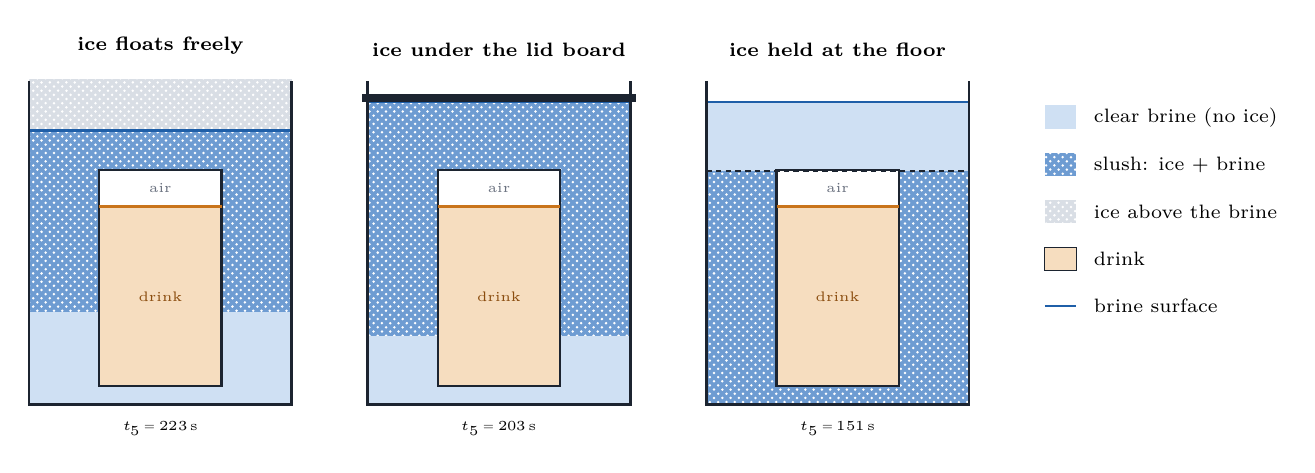
\begin{tikzpicture}
\begin{scope}[shift={(0.00,0)}, x=0.235cm, y=0.235cm]
\path[fill=cBrine] (0,0.00) rectangle (14.2,4.98);
\path[fill=cSlush, postaction={pattern=crosshatch dots, pattern color=white}] (0,4.98) rectangle (14.2,14.81);
\path[fill=cDry, postaction={pattern=crosshatch dots, pattern color=white}] (0,14.81) rectangle (14.2,17.60);
\draw[cBlue, thick] (0,14.81) -- (14.2,14.81);
\fill[white] (3.80,1.00) rectangle (10.40,12.66);
\fill[cAmberLight] (3.80,1.00) rectangle (10.40,10.70);
\draw[cInk, line width=0.8pt] (3.80,1.00) rectangle (10.40,12.66);
\draw[cAmber, thick] (3.80,10.70) -- (10.40,10.70);
\node[font=\tiny, cAmberDark] at (7.10,5.85) {drink};
\node[font=\tiny, cGrey] at (7.10,11.68) {air};
\draw[cInk, line width=1pt] (0,17.50) -- (0,0) -- (14.2,0) -- (14.2,17.50);
\node[font=\scriptsize\bfseries, anchor=south] at (7.10,18.40) {ice floats freely};
\node[font=\tiny, anchor=north, align=center] at (7.10,-0.4) {$t_5=223$\,s};
\end{scope}
\begin{scope}[shift={(4.30,0)}, x=0.235cm, y=0.235cm]
\path[fill=cBrine] (0,0.00) rectangle (14.2,3.72);
\path[fill=cSlush, postaction={pattern=crosshatch dots, pattern color=white}] (0,3.72) rectangle (14.2,16.35);
\draw[cBlue, thick] (0,16.35) -- (14.2,16.35);
\fill[white] (3.80,1.00) rectangle (10.40,12.66);
\fill[cAmberLight] (3.80,1.00) rectangle (10.40,10.70);
\draw[cInk, line width=0.8pt] (3.80,1.00) rectangle (10.40,12.66);
\draw[cAmber, thick] (3.80,10.70) -- (10.40,10.70);
\node[font=\tiny, cAmberDark] at (7.10,5.85) {drink};
\node[font=\tiny, cGrey] at (7.10,11.68) {air};
\fill[cInk] (-0.3,16.35) rectangle (14.5,16.80);
\draw[cInk, line width=1pt] (0,17.50) -- (0,0) -- (14.2,0) -- (14.2,17.50);
\node[font=\scriptsize\bfseries, anchor=south] at (7.10,18.30) {ice under the lid board};
\node[font=\tiny, anchor=north, align=center] at (7.10,-0.4) {$t_5=203$\,s};
\end{scope}
\begin{scope}[shift={(8.60,0)}, x=0.235cm, y=0.235cm]
\path[fill=cSlush, postaction={pattern=crosshatch dots, pattern color=white}] (0,0.00) rectangle (14.2,12.63);
\path[fill=cBrine] (0,12.63) rectangle (14.2,16.35);
\draw[cBlue, thick] (0,16.35) -- (14.2,16.35);
\fill[white] (3.80,1.00) rectangle (10.40,12.66);
\fill[cAmberLight] (3.80,1.00) rectangle (10.40,10.70);
\draw[cInk, line width=0.8pt] (3.80,1.00) rectangle (10.40,12.66);
\draw[cAmber, thick] (3.80,10.70) -- (10.40,10.70);
\node[font=\tiny, cAmberDark] at (7.10,5.85) {drink};
\node[font=\tiny, cGrey] at (7.10,11.68) {air};
\draw[cInk, thick, dash pattern=on 2pt off 1.5pt] (0,12.63) -- (14.2,12.63);
\draw[cInk, line width=1pt] (0,17.50) -- (0,0) -- (14.2,0) -- (14.2,17.50);
\node[font=\scriptsize\bfseries, anchor=south] at (7.10,18.30) {ice held at the floor};
\node[font=\tiny, anchor=north, align=center] at (7.10,-0.4) {$t_5=151$\,s};
\end{scope}
\begin{scope}[shift={(12.9,0.6)}, font=\scriptsize]
\path[fill=cBrine] (0,2.9) rectangle (0.4,3.2); \node[anchor=west] at (0.5,3.05) {clear brine (no ice)};
\path[fill=cSlush, postaction={pattern=crosshatch dots, pattern color=white}] (0,2.3) rectangle (0.4,2.6); \node[anchor=west] at (0.5,2.45) {slush: ice + brine};
\path[fill=cDry, postaction={pattern=crosshatch dots, pattern color=white}] (0,1.7) rectangle (0.4,2.0); \node[anchor=west] at (0.5,1.85) {ice above the brine};
\path[fill=cAmberLight, draw=cInk] (0,1.1) rectangle (0.4,1.4); \node[anchor=west] at (0.5,1.25) {drink};
\draw[cBlue, thick] (0,0.65) -- (0.4,0.65); \node[anchor=west] at (0.5,0.65) {brine surface};
\end{scope}
\end{tikzpicture}
\caption{Your tank drawn to scale after recipe B1 has settled (\val{B1mi}\,kg ice, \val{B1mw}\,kg water, \val{B1ms}\,kg salt). Ice floats in brine, so where it ends up depends on how you hold it. Left: free-floating ice leaves \val{B1Flhcb}\,cm of clear (ice-free) brine at the bottom. Middle: ice pushed under a lid board. Right: ice held down on the floor by a mesh, with the clear brine on top. The can's drink (amber) fills \val{Ctwohd}\,mm of its \val{CtwoH}\,mm height; the rest is air. Times are for 25\,$\to$\,5\,\textdegree C from \S\ref{sec:heat}.}
\label{fig:tank}
\end{figure}

\subsection{The variables}
\textbf{Control variables} (what you change between runs):

\begin{center}\small
\begin{tabular}{@{}l l l@{}}
\toprule
symbol & meaning & enters as \\
\midrule
\inp\ $m_w$ & mass of liquid water added, at $T_r$ & sensible heat; solvent \\
\inp\ $m_s$ & mass of NaCl added, at $T_r$ & solute; dissolution heat \\
\inp\ $m_e$ & mass of ethanol added, at $T_r$ & solute; heat of mixing \\
\inp\ $m_i$ & mass of ice added, at $0$\,\textdegree C & latent-heat store \\
\bottomrule
\end{tabular}
\end{center}

\textbf{Measured or tabulated once} (\meas). Values are the ones used for every number in this document.

\begin{center}\footnotesize
\renewcommand{\arraystretch}{1.12}
\begin{tabularx}{\linewidth}{@{}l X r l@{}}
\toprule
symbol & meaning & value & how to get it \\
\midrule
\multicolumn{4}{@{}l}{\textit{thermodynamics}}\\
$c_w,\;c_i,\;c_s,\;c_e$ & specific heats: water, ice, NaCl (solid), pure ethanol (0--25\,\textdegree C) & $\val{cw},\;\val{ci},\;\val{cs},\;\val{ce}$\,J\,kg$^{-1}$K$^{-1}$ & handbook \\
$L_0$ & latent heat of fusion of ice at 0\,\textdegree C & $\val{Lzero}$\,kJ/kg & handbook \\
$\Delta c=c_w-c_i$ & makes the latent heat temperature dependent, $L(\theta)=L_0-\Delta c\,\theta$ & $\val{dc}$\,J\,kg$^{-1}$K$^{-1}$ & derived \\
$\Delta h_s$ & molar enthalpy of solution of NaCl (endothermic) & $\val{dhs}$\,kJ/mol & handbook (placeholder) \\
$h_E(b_e)$ & heat of mixing per mole of ethanol at 0\,\textdegree C, $h_E=h_\infty+g\,b_e$ & $h_\infty=\val{hEinf}$\,kJ/mol, $g=\val{hEg}$ & fitted to $H^E$ table \\
$c_{ea}(b_e)$ & apparent specific heat of ethanol dissolved in water below 0\,\textdegree C & $\min(\val{ceaCap},\,\val{ceaZero}\val{ceaSl}\,b_e)$\,kJ\,kg$^{-1}$K$^{-1}$ & fitted to Melinder \\
$M_s,\;M_e$ & molar masses of NaCl, ethanol & $\val{Ms},\;\val{Me}$\,g/mol & \\
\multicolumn{4}{@{}l}{\textit{liquidus (freezing-point) constants, fitted in \S\ref{sec:liq}}}\\
$K_s,\;\omega_s$ & NaCl: depression constant and bound water per mole & $\val{Ks}$\,K\,kg/mol, $\val{oms}$\,kg/mol & Bodnar (1993) \\
$K_e,\;\omega_e$ & ethanol: depression constant, bound water & $\val{Ke}$\,K\,kg/mol, 0 & Lange, Melinder \\
$b_E,\;\theta_E$ & eutectic brine molality and depression & $\val{bE}$\,mol/kg, $\val{thE}$\,K & Bodnar (1993) \\
$\lambda$ & drop in NaCl solubility per mol/kg of ethanol (along the cotectic) & $\val{lam}$\,kg/mol & NIST ThermoML \\
\multicolumn{4}{@{}l}{\textit{mixing}}\\
$\eta_s,\;\eta_e$ & fraction of the salt / ethanol that actually reaches the liquid around the ice & 1 (perfect) & \S\ref{sec:eta}: from $T_b$ \\
\multicolumn{4}{@{}l}{\textit{slush, brine, drink, can, tank}}\\
$\varphi_p$ & volume fraction of ice in the packed slush & $\val{phip}$ & weigh ice in a known volume \\
$\rho_i,\;k_i$ & ice density, conductivity & $\val{rhoi}$\,kg/m$^3$, $\val{ki}$\,W\,m$^{-1}$K$^{-1}$ & handbook \\
$k_b,\;k_l$ & conductivity of cold brine; of the diluted melt next to the can & $\val{kb},\;\val{kl}$\,W\,m$^{-1}$K$^{-1}$ & handbook \\
$\rho_0,\beta_s,\beta_e$ & brine density $\rho_b=\rho_0+\beta_s w_s-\beta_e w_e$ & $1000,\;\val{betas},\;\val{betae}$\,kg/m$^3$ & weigh 100\,mL of brine \\
$\rho_d,\;c_d,\;k_d$ & drink density, specific heat, conductivity & $\val{rhod},\;\val{cd},\;\val{kd}$ & 10\,wt\% sugar solution \\
$R,\;H,\;t_w,\;m_{\rm Al}$ & can: outer radius, height, wall thickness, empty mass & \val{CtwoR}, \val{CtwoH}, \val{tw}\,mm; \val{mAl}\,g & callipers, balance \\
$V_d$ & volume of drink in the can & 330\,mL & weigh full and empty \\
$k_{\rm Al},\;c_{\rm Al}$ & aluminium & $\val{kAl}$\,W\,m$^{-1}$K$^{-1}$, $\val{cAl}$\,J\,kg$^{-1}$K$^{-1}$ & handbook \\
$A_t,\;H_t,\;z_0$ & tank floor area and height; height of the can base above the floor & $\val{At}$\,cm$^2$, $\val{Ht}$\,cm, $\val{zzero}$\,cm & ruler \\
$T_r,\;T_0,\;T_1$ & room temperature; drink start; target & $\val{Tzero}$, $\val{Tzero}$, $\val{Tone}$\,\textdegree C & thermometer \\
\bottomrule
\end{tabularx}
\end{center}

Everything else is \der{} \emph{derived}. Each derived quantity is defined by one numbered equation, in the order in which you evaluate them (the full list is in \S\ref{sec:chain}).

\subsection{Assumptions}\label{sec:assump}
\begin{enumerate}[label=\textbf{A\arabic*},leftmargin=2.2em]
\item The bath reaches equilibrium before the can goes in (without a stirrer this takes a while; see A4). The tank exchanges no heat with the room during one run; a heat leak can be added as a known heat $Q_x$ in Eq.~\eqref{eq:energy}.
\item Heat capacities are constant within each step of the energy bookkeeping. The ethanol heat of mixing and apparent heat capacity depend on concentration and are updated once (a two-pass evaluation, \S\ref{sec:twopass}).
\item The ice liquidus of the mixed brine follows the Zdanovskii--Stokes--Robinson (ZSR) water-activity rule, with each binary liquidus written in a form fitted to data (\S\ref{sec:liq}).
\item Imperfect mixing: only the fractions $\eta_s$ and $\eta_e$ of the salt and ethanol are dissolved in the liquid that touches the ice. The rest stays apart (salt crust on the floor, an ethanol layer on top).
\item \textbf{No convection in the bath.} Heat moves only by conduction. Dissolved salt and ethanol do not move during a run: their diffusion is about 90 times slower than heat diffusion (\S\ref{sec:noconv}).
\item The drink is well mixed (one temperature $T_d$) in the main model. The limit in which the drink cannot convect either is treated in \S\ref{sec:conduct}.
\item The can is a cylinder with a 0.1\,mm aluminium wall, whose resistance ($t_w/k_{\rm Al}\approx5\times10^{-7}$\,m$^2$K/W) is negligible. Its dome, neck and coatings are ignored. The air space conducts no heat.
\item Ice packs with ice volume fraction $\varphi_p$, and brine fills the pores below the brine surface. The part of the can above the brine surface exchanges no heat (ice touching dry aluminium through air).
\item On the time scale of one cooling the slush and brine around the can act as unbounded. The thermal disturbance reaches about 2\,cm, less than the 3.8\,cm clearance to the tank wall.
\item The drink (about 10\,wt\% sugar) does not freeze in the main model. Its freezing point is $-0.77$\,\textdegree C; see \S\ref{sec:conduct} for when the wall goes colder than that.
\end{enumerate}

\begin{center}
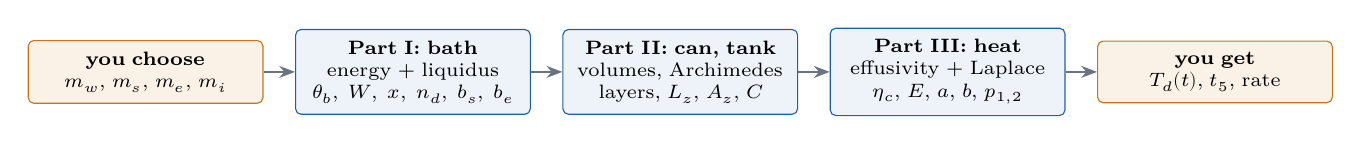
\begin{tikzpicture}[node distance=4mm, box/.style={draw=cBlue, fill=cBlueBg, rounded corners=2pt, align=center, font=\scriptsize, inner sep=4pt, text width=27mm},
  inbox/.style={box, draw=cAmber, fill=cAmberBg}, arr/.style={-{Stealth[length=2mm]}, thick, cGrey}]
\node[inbox] (in) {\textbf{you choose}\\ $m_w,\,m_s,\,m_e,\,m_i$};
\node[box, right=of in] (b) {\textbf{Part I: bath}\\ energy + liquidus\\ $\theta_b,\;W,\;x,\;n_d,\;b_s,\;b_e$};
\node[box, right=of b] (g) {\textbf{Part II: can, tank}\\ volumes, Archimedes\\ layers, $L_z$, $A_z$, $C$};
\node[box, right=of g] (h) {\textbf{Part III: heat}\\ effusivity + Laplace\\ $\eta_c,\,E,\,a,\,b,\,p_{1,2}$};
\node[inbox, right=of h] (o) {\textbf{you get}\\ $T_d(t)$, $t_5$, rate};
\draw[arr] (in) -- (b); \draw[arr] (b) -- (g); \draw[arr] (g) -- (h); \draw[arr] (h) -- (o);
\end{tikzpicture}
\end{center}

% =====================================================================================================
\section{Part I \,\textperiodcentered\, The bath in closed form}\label{sec:bath}

\begin{plain}[What decides the bath temperature]
Two conditions must hold at the same time.
\begin{itemize}
\item \textbf{Energy.} The heat that the warm water, salt and ethanol bring in, plus the heat of solution and of mixing, has nowhere to go but into melting ice.
\item \textbf{Phase equilibrium.} Ice can only sit in a liquid that is on its \emph{liquidus}: the more dissolved solute per kilogram of liquid water, the colder that liquid must be.
\end{itemize}
Melting ice adds water and dilutes the brine, so the two conditions pull against each other. Solving them together gives one temperature.
\end{plain}

\textbf{Notation.} Write the bath temperature as a depression below 0\,\textdegree C, $\theta\equiv-T_b$ (in K, positive when colder than 0\,\textdegree C). $W$ is the mass of liquid water in the bath at the end, $x=W-m_w$ the mass of ice that melted, and $n_d$ the moles of salt dissolved.

\subsection{The mixing coefficient}\label{sec:eta}
With no stirrer, some of the salt you pour in never meets the ice: it sinks as a crust, or sits in a pocket of already saturated brine. Ethanol is lighter than brine and can float as a layer. Let the fractions that do end up in the liquid touching the ice be $\eta_s$ and $\eta_e$ (between 0 and 1). The \emph{active} amounts are
\begin{equation}
n_s'=\eta_s\,\frac{m_s}{M_s},\qquad n_e'=\eta_e\,\frac{m_e}{M_e}.
\label{eq:active}
\end{equation}
This is the ``lowered coefficient'' in its simplest form. In every formula below only $n_s'$ and $n_e'$ lower the freezing point and absorb or release heat of solution, so the effective depression constant per kilogram of salt you added drops from $K_s/M_s$ to $\eta_sK_s/M_s$. The inactive salt still has to be cooled, so it stays in the heat capacities. How to measure $\eta_s$ is in \S\ref{sec:etainv}.

\subsection{Energy balance}\label{sec:energy}
Enthalpy is a function of state, so any imaginary path from the start to the end gives the same answer. Take this one:
\begin{enumerate}[label=(\roman*)]
\item cool the water, salt and ethanol from $T_r$ to 0\,\textdegree C, releasing $C_r\,\Delta T_r$;
\item at 0\,\textdegree C, melt $x$ of ice (absorbs $xL_0$), dissolve $n_d$ moles of salt (absorbs $n_d\Delta h_s$), and mix $n_e'$ moles of ethanol into the water (absorbs $n_e'h_E$; $h_E<0$, so it actually releases heat);
\item cool everything from 0\,\textdegree C to $-\theta$, releasing $\theta\,[\,(m_w+x)c_w+(m_i-x)c_i+m_sc_s+\eta_em_ec_{ea}+(1-\eta_e)m_ec_e\,]$.
\end{enumerate}
In an insulated tank, heat released equals heat absorbed. Collecting the terms in $x$:
\begin{equation}
\boxed{\;x\,(L_0-\Delta c\,\theta)=C_r\,\Delta T_r+C_\theta\,\theta-n_d\,\Delta h_s-n_e'\,h_E+Q_x\;}
\label{eq:energy}
\end{equation}
\begin{equation}
C_r=m_wc_w+m_sc_s+m_ec_e,\qquad C_\theta=m_wc_w+m_sc_s+\eta_em_ec_{ea}+(1-\eta_e)m_ec_e+m_ic_i,\qquad \Delta T_r=T_r-0\,\text{\textdegree C}.
\label{eq:Cs}
\end{equation}
Reading Eq.~\eqref{eq:energy} term by term:
\begin{itemize}
\item \textbf{left side:} the heat needed to melt $x$ of ice at the bath temperature. $L_0-\Delta c\,\theta$ is the latent heat at $-\theta$ (Kirchhoff's law): \val{Lzero}\,kJ/kg at 0\,\textdegree C, about 13\,\% less at the eutectic.
\item \textbf{$C_r\Delta T_r$:} the heat the warm inputs bring.
\item \textbf{$C_\theta\theta$:} the heat released as everything cools below 0\,\textdegree C. This includes the ice, which starts at 0\,\textdegree C and must be cooled too.
\item \textbf{$n_d\Delta h_s$:} the heat dissolution of salt takes.
\item \textbf{$-n_e'h_E$:} the heat mixing ethanol gives.
\item \textbf{$Q_x$:} any extra heat in (heat leak, or the can's heat; 0 for the bath alone).
\end{itemize}

\subsection{The liquidus with bound water}\label{sec:liq}
\textbf{Why not Blagden's law.} $\theta=iK_fb$ with $i=2$ assumes an ideal, dilute solution. Against Bodnar's (1993) measured NaCl liquidus it is wrong by up to $\val{BlagErr}$\,K: too cold below about 16\,wt\% and too warm above, because the ions are not ideal.

\textbf{A form that fits and keeps the algebra closed.} Suppose each mole of solute ties up $\omega$ kilograms of water in its hydration shell, so that only $W-\omega n$ of the liquid water acts as free solvent. A dilute-law depression on the free water then reads
\begin{equation}
\theta=\frac{K\,n}{W-\omega\,n}\quad\Longleftrightarrow\quad \theta=\frac{K\,b}{1-\omega\,b},\qquad b=\frac nW .
\label{eq:binary}
\end{equation}
Fitted to Bodnar's liquidus and forced through the eutectic ($b_E=\val{bE}$\,mol/kg at $\theta_E=\val{thE}$\,K), NaCl gives $K_s=\val{Ks}$\,K\,kg/mol and $\omega_s=\val{oms}$\,kg/mol. That is $\val{omsH}$ water molecules per NaCl, and the worst error from 0 to $-21.2$\,\textdegree C is \val{HypErr}\,K, against \val{BlagErr}\,K for Blagden. For ethanol the fitted $\omega_e$ comes out as zero (it is not an ion), leaving $\theta=K_eb_e$ with $K_e=\val{Ke}$\,K\,kg/mol (worst error \val{EtohErr}\,K over 0--28\,K; Fig.~\ref{fig:liq}).

\textbf{Mixing the two (ZSR).} The ZSR rule says a mixed brine freezes at the temperature where each solute's share of ``water activity'' adds up. If $b_{j,0}(\theta)$ is the molality of solute $j$ alone that freezes at $\theta$, then $\sum_j b_j/b_{j,0}(\theta)=1$. Inverting Eq.~\eqref{eq:binary} gives $b_{j,0}=\theta/(K_j+\omega_j\theta)$, so
\[
\frac{b_s(K_s+\omega_s\theta)+b_e(K_e+\omega_e\theta)}{\theta}=1
\quad\Longrightarrow\quad
\theta=\frac{K_sb_s+K_eb_e}{1-\omega_sb_s-\omega_eb_e}.
\]
With $b=n/W$:
\begin{equation}
\boxed{\;\theta\,(W-W_b)=N,\qquad N=K_s\,n_s'+K_e\,n_e',\qquad W_b=\omega_s\,n_s'+\omega_e\,n_e'\;}
\label{eq:liq}
\end{equation}
$N$ (in K\,kg) is the ``depression strength'' of what is dissolved. $W_b$ is the bound water. Against the numerical ZSR model built on the full data tables, Eq.~\eqref{eq:liq} is within \val{ZsrMax}\,K everywhere (rms \val{ZsrRms}\,K), and the worst case is at $-30$\,\textdegree C.

\begin{figure}[H]
\centering

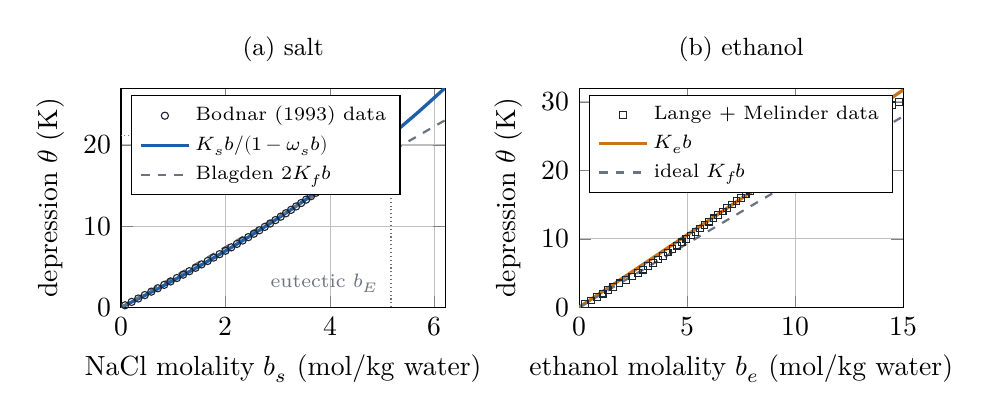
\begin{tikzpicture}
\begin{groupplot}[group style={group size=2 by 1, horizontal sep=17mm}, width=0.47\linewidth, height=0.36\linewidth,
  ylabel={depression $\theta$ (K)}, ymin=0, grid=major, legend cell align=left, legend style={font=\scriptsize, at={(0.03,0.97)}, anchor=north west}]
\nextgroupplot[xlabel={NaCl molality $b_s$ (mol/kg water)}, xmin=0, xmax=6.2, ymax=27, title={\small (a) salt}]
\addplot[only marks, mark=o, mark size=1.3pt, cInk] coordinates {(0.07601,0.25) (0.2031,0.6701) (0.3294,1.09) (0.4548,1.51) (0.5794,1.93) (0.703,2.35) (0.8258,2.77) (0.9475,3.19) (1.068,3.61) (1.188,4.03) (1.307,4.451) (1.425,4.871) (1.541,5.291) (1.657,5.711) (1.771,6.131) (1.884,6.551) (1.997,6.971) (2.108,7.391) (2.217,7.811) (2.326,8.231) (2.434,8.651) (2.54,9.071) (2.645,9.491) (2.749,9.911) (2.852,10.33) (2.954,10.75) (3.054,11.17) (3.153,11.59) (3.252,12.01) (3.349,12.43) (3.445,12.85) (3.54,13.27) (3.633,13.69) (3.726,14.11) (3.818,14.53) (3.909,14.95) (3.998,15.37) (4.087,15.79) (4.175,16.21) (4.262,16.63) (4.348,17.05) (4.434,17.47) (4.518,17.89) (4.602,18.31) (4.685,18.73) (4.768,19.15) (4.85,19.57) (4.931,19.99) (5.012,20.41) (5.093,20.83)};
\addlegendentry{Bodnar (1993) data}
\addplot[cBlue, very thick] coordinates {(0,0) (0.1,0.3187) (0.2,0.6403) (0.3,0.9647) (0.4,1.292) (0.5,1.622) (0.6,1.956) (0.7,2.292) (0.8,2.631) (0.9,2.974) (1,3.319) (1.1,3.668) (1.2,4.02) (1.3,4.376) (1.4,4.734) (1.5,5.096) (1.6,5.462) (1.7,5.831) (1.8,6.203) (1.9,6.579) (2,6.959) (2.1,7.342) (2.2,7.73) (2.3,8.12) (2.4,8.515) (2.5,8.914) (2.6,9.316) (2.7,9.723) (2.8,10.13) (2.9,10.55) (3,10.97) (3.1,11.39) (3.2,11.82) (3.3,12.25) (3.4,12.69) (3.5,13.13) (3.6,13.57) (3.7,14.02) (3.8,14.48) (3.9,14.94) (4,15.4) (4.1,15.87) (4.2,16.35) (4.3,16.83) (4.4,17.31) (4.5,17.81) (4.6,18.3) (4.7,18.8) (4.8,19.31) (4.9,19.82) (5,20.34) (5.1,20.87) (5.2,21.4) (5.3,21.93) (5.4,22.48) (5.5,23.03) (5.6,23.58) (5.7,24.14) (5.8,24.71) (5.9,25.29) (6,25.87) (6.1,26.46) (6.2,27.06)};
\addlegendentry{$K_s b/(1-\omega_s b)$}
\addplot[cGrey, dashed, thick] coordinates {(0,0) (0.1,0.372) (0.2,0.744) (0.3,1.116) (0.4,1.488) (0.5,1.86) (0.6,2.232) (0.7,2.604) (0.8,2.976) (0.9,3.348) (1,3.72) (1.1,4.092) (1.2,4.464) (1.3,4.836) (1.4,5.208) (1.5,5.58) (1.6,5.952) (1.7,6.324) (1.8,6.696) (1.9,7.068) (2,7.44) (2.1,7.812) (2.2,8.184) (2.3,8.556) (2.4,8.928) (2.5,9.3) (2.6,9.672) (2.7,10.04) (2.8,10.42) (2.9,10.79) (3,11.16) (3.1,11.53) (3.2,11.9) (3.3,12.28) (3.4,12.65) (3.5,13.02) (3.6,13.39) (3.7,13.76) (3.8,14.14) (3.9,14.51) (4,14.88) (4.1,15.25) (4.2,15.62) (4.3,16) (4.4,16.37) (4.5,16.74) (4.6,17.11) (4.7,17.48) (4.8,17.86) (4.9,18.23) (5,18.6) (5.1,18.97) (5.2,19.34) (5.3,19.72) (5.4,20.09) (5.5,20.46) (5.6,20.83) (5.7,21.2) (5.8,21.58) (5.9,21.95) (6,22.32) (6.1,22.69) (6.2,23.06)};
\addlegendentry{Blagden $2K_f b$}
\draw[cGrey, densely dotted] (axis cs:5.163,0) -- (axis cs:5.163,21.2) -- (axis cs:0,21.2);
\node[font=\scriptsize, anchor=east, cGrey] at (axis cs:5.1,3) {eutectic $b_E$};
\nextgroupplot[xlabel={ethanol molality $b_e$ (mol/kg water)}, xmin=0, xmax=15, ymax=32, title={\small (b) ethanol}]
\addplot[only marks, mark=square, mark size=1.2pt, cInk] coordinates {(0.2805,0.5) (0.5566,1) (0.8298,1.5) (1.094,2) (1.337,2.5) (1.584,3) (1.874,3.5) (2.183,4) (2.464,4.5) (2.719,5) (2.962,5.5) (3.197,6) (3.426,6.5) (3.651,7) (3.876,7.5) (4.098,8) (4.317,8.5) (4.533,9) (4.748,9.5) (4.96,10) (5.172,10.5) (5.384,11) (5.596,11.5) (5.807,12) (6.016,12.5) (6.225,13) (6.434,13.5) (6.643,14) (6.853,14.5) (7.065,15) (7.279,15.5) (7.493,16) (7.708,16.5) (7.923,17) (8.139,17.5) (8.357,18) (8.577,18.5) (8.8,19) (9.026,19.5) (9.256,20) (9.49,20.5) (9.725,21) (9.963,21.5) (10.2,22) (10.45,22.5) (10.7,23) (10.95,23.5) (11.21,24) (11.47,24.5) (11.74,25) (12.02,25.5) (12.3,26) (12.59,26.5) (12.89,27) (13.19,27.5) (13.5,28) (13.81,28.5) (14.14,29) (14.47,29.5) (14.81,30)};
\addlegendentry{Lange + Melinder data}
\addplot[cAmber, very thick] coordinates {(0,0) (0.5,1.058) (1,2.116) (1.5,3.174) (2,4.232) (2.5,5.29) (3,6.348) (3.5,7.406) (4,8.465) (4.5,9.523) (5,10.58) (5.5,11.64) (6,12.7) (6.5,13.75) (7,14.81) (7.5,15.87) (8,16.93) (8.5,17.99) (9,19.05) (9.5,20.1) (10,21.16) (10.5,22.22) (11,23.28) (11.5,24.34) (12,25.39) (12.5,26.45) (13,27.51) (13.5,28.57) (14,29.63) (14.5,30.68) (15,31.74)};
\addlegendentry{$K_e b$}
\addplot[cGrey, dashed, thick] coordinates {(0,0) (0.5,0.93) (1,1.86) (1.5,2.79) (2,3.72) (2.5,4.65) (3,5.58) (3.5,6.51) (4,7.44) (4.5,8.37) (5,9.3) (5.5,10.23) (6,11.16) (6.5,12.09) (7,13.02) (7.5,13.95) (8,14.88) (8.5,15.81) (9,16.74) (9.5,17.67) (10,18.6) (10.5,19.53) (11,20.46) (11.5,21.39) (12,22.32) (12.5,23.25) (13,24.18) (13.5,25.11) (14,26.04) (14.5,26.97) (15,27.9)};
\addlegendentry{ideal $K_f b$}
\end{groupplot}
\end{tikzpicture}
\caption{The two liquidus fits. (a) NaCl: the bound-water form follows Bodnar's data to \val{HypErr}\,K; Blagden's law misses by up to \val{BlagErr}\,K. (b) Ethanol: a straight line $K_eb_e$ with an effective $K_e=\val{Ke}$ (ideal: 1.86).}
\label{fig:liq}
\end{figure}

\subsection{Regime U: salt all dissolved, ice left}\label{sec:U}
All the active salt is in solution, $n_d=n_s'$, and $W=m_w+x$. Eq.~\eqref{eq:liq} gives $W=W_b+N/\theta$. Substituting this into Eq.~\eqref{eq:energy} and multiplying by $\theta\,(L_0-\Delta c\,\theta)$ leaves a quadratic in $\theta$:
\begin{equation}
A\,\theta^2+B\,\theta-N L_0=0,\qquad
\begin{aligned}
A&=C_\theta-\Delta c\,(m_w-W_b),\\
B&=(m_w-W_b)\,L_0+Q_0+\Delta c\,N,\\
Q_0&=C_r\Delta T_r-n_s'\Delta h_s-n_e'h_E+Q_x .
\end{aligned}
\label{eq:quad}
\end{equation}
$A>0$ (it equals $m_wc_i+m_sc_s+m_e[\eta_ec_{ea}+(1-\eta_e)c_e]+m_ic_i+\Delta c\,W_b$) and $NL_0>0$, so exactly one root is positive:
\begin{equation}
\boxed{\;\theta_U=\frac{2NL_0}{B+\sqrt{B^2+4ANL_0}}\;},\qquad T_b=-\theta_U,\qquad W=W_b+\frac{N}{\theta_U},\qquad x=W-m_w .
\label{eq:thetaU}
\end{equation}
(This form avoids the cancellation in $(-B+\sqrt{\cdot})/2A$.) It holds while two checks pass: ice is left ($x\le m_i$), and the brine is not saturated ($n_s'\le b_E\,(W-\lambda n_e')$, see Eq.~\eqref{eq:cot}). If $N=0$ (plain ice water), $\theta=0$ and $x=Q_0/L_0$.

\subsection{Regime S: saturated, solid salt and ice both left}\label{sec:S}
\textbf{Salt only: the eutectic.} Ice, solid salt and brine coexist: three phases of two components, so the phase rule gives $F=C-P+1=2-3+1=0$ degrees of freedom. The temperature is pinned at $\theta=\theta_E$ and the brine at $b_E$, so $n_d=b_EW$. Eq.~\eqref{eq:energy} becomes linear in $W$:
\begin{equation}
\boxed{\;W_S=\frac{m_wL_E+C_r\Delta T_r+C_\theta\theta_E+Q_x}{L_E+b_E\Delta h_s}\;},\qquad L_E=L_0-\Delta c\,\theta_E,\qquad m_{\rm salt,left}=m_s-b_EW_SM_s .
\label{eq:WS}
\end{equation}
\textbf{With ethanol: the cotectic.} Three components and three phases give $F=1$, so the temperature now drifts with the ethanol content. Two facts fix it. Per kilogram of water, salt is less soluble when ethanol is present, $b_{\rm sat}=b_E(1-\lambda b_e)$, so $n_d=b_E(W-\lambda n_e')$. Put that into Eq.~\eqref{eq:liq}:
\begin{equation}
\theta=\frac{PW+P'}{QW+Q'},\qquad P=K_sb_E,\quad P'=n_e'(K_e-\lambda K_sb_E),\quad Q=1-\omega_sb_E,\quad Q'=n_e'(\lambda\omega_sb_E-\omega_e).
\label{eq:cot}
\end{equation}
Multiplying Eq.~\eqref{eq:energy} by $QW+Q'$ gives a quadratic $a_2W^2+a_1W+a_0=0$:
\begin{equation}
\begin{aligned}
a_2&=\alpha_1+b_E\Delta h_sQ, & \alpha_1&=L_0Q-\Delta c\,P,\\
a_1&=\alpha_0-m_w\alpha_1-C_\theta P+b_E\Delta h_sQ'-GQ, & \alpha_0&=L_0Q'-\Delta c\,P',\\
a_0&=-m_w\alpha_0-C_\theta P'-GQ', & G&=C_r\Delta T_r+\lambda b_En_e'\Delta h_s-n_e'h_E+Q_x .
\end{aligned}
\label{eq:cotquad}
\end{equation}
Since $a_2>0$ and $a_0<0$, there is one positive root, $W_S=\big(-a_1+\sqrt{a_1^2-4a_2a_0}\big)/2a_2$, and $\theta_S$ follows from Eq.~\eqref{eq:cot}. With $n_e'=0$ this reduces exactly to Eq.~\eqref{eq:WS}. The cotectic constant $\lambda=\val{lam}$\,kg/mol reproduces the NIST solubility data within \val{bsatRel}\,\%. The cotectic temperature then agrees with the numerical model to \val{CotErr}\,K.

\subsection{Regime I: the ice is all gone}\label{sec:I}
If the heat brought in is more than the ice can absorb, $x=m_i$ and $W=m_w+m_i$. Eq.~\eqref{eq:energy} then gives the temperature directly:
\begin{equation}
\theta_I=\frac{m_iL_0-C_r\Delta T_r+n_d\Delta h_s+n_e'h_E-Q_x}{C_\theta+m_i\Delta c}\qquad(\theta_I<0 \text{ means above }0\,\text{\textdegree C}).
\label{eq:thetaI}
\end{equation}
A bath in regime I has no latent-heat store left, so it is useless for cooling a drink.

\subsection{Which regime? Boundaries in closed form}\label{sec:bounds}
Evaluate Eq.~\eqref{eq:thetaU} first. If its two checks pass, that is the answer. If the brine comes out saturated, use regime S. If $x>m_i$, use regime I. Because the bath's enthalpy rises monotonically with the ice melted, exactly one regime is consistent. Setting the checks to equalities gives the boundaries as explicit formulas.

\textbf{Salt needed to reach the eutectic} (salt only). Put $\theta=\theta_E$ and $W=n_s'/b_E$ into Eq.~\eqref{eq:energy}. Both $C_r$ and $C_\theta$ are linear in $m_s$, so
\begin{equation}
m_s^{\ast}=\frac{m_w\,[L_E+c_w(\Delta T_r+\theta_E)]+m_ic_i\theta_E}{\eta_s\,(L_E+b_E\Delta h_s)/(M_sb_E)-c_s(\Delta T_r+\theta_E)} .
\label{eq:mstar}
\end{equation}
For B1 ($m_w=\val{B1mw}$, $m_i=\val{B1mi}$\,kg) this is \val{SatBone}\,kg, so B1's \val{B1ms}\,kg is just enough and leaves \val{B1solid}\,g of solid salt. For your original charge B4 it is \val{SatBfour}\,kg: the \val{B4ms}\,kg you planned never reaches the eutectic and the bath sits at $\val{B4Tbone}$\,\textdegree C. This is the same ``mass balance is not an energy balance'' point as the 24~Oct note.

\textbf{Ethanol that melts all the ice.} Set $x=m_i$ in Eq.~\eqref{eq:energy} and in Eq.~\eqref{eq:liq} or Eq.~\eqref{eq:cot}. In the unsaturated branch $\theta=N/(m_w+m_i-W_b)$ is linear in $m_e$, so the energy balance becomes a quadratic in $m_e$; the saturated branch also reduces to a quadratic. For B1's water, salt and ice the ice is gone at $m_e=\val{ExBoneme}$\,kg ($T_b=\val{ExBoneT}$\,\textdegree C). For B2's at \val{ExBtwome}\,kg ($\val{ExBtwoT}$\,\textdegree C), and for ethanol alone at \val{ExBthreeme}\,kg ($\val{ExBthreeT}$\,\textdegree C).
\begin{warn}[These are limits, not recipes]
At those points the bath has no ice left, and the temperatures are below $-23.6$\,\textdegree C, where the NaCl liquidus is extrapolated (unreliable below $-27$\,\textdegree C). The practical floors are the regime-S values with ice to spare.
\end{warn}

\subsection{How sensitive is the bath? Closed-form derivatives}\label{sec:sens}
Differentiate $F(\theta)=A\theta^2+B\theta-NL_0=0$ implicitly. $A$, $B$ and $N$ are all linear in each mass, so for any input $m_j$
\begin{equation}
\frac{\partial\theta}{\partial m_j}=\frac{L_0\,\partial_jN-\theta^2\,\partial_jA-\theta\,\partial_jB}{2A\theta+B},
\label{eq:sens}
\end{equation}
with the partial derivatives
\begin{center}\small
\begin{tabular}{@{}l c c c@{}}
\toprule
input & $\partial_jN$ & $\partial_jA$ & $\partial_jB$ \\
\midrule
$m_w$ & 0 & $c_i$ & $L_0+c_w\Delta T_r$ \\
$m_i$ & 0 & $c_i$ & 0 \\
$m_s$ & $\eta_sK_s/M_s$ & $c_s+\Delta c\,\eta_s\omega_s/M_s$ & $c_s\Delta T_r+(\eta_s/M_s)(\Delta c\,K_s-\omega_sL_0-\Delta h_s)$ \\
$m_e$ & $\eta_eK_e/M_e$ & $\eta_ec_{ea}+(1-\eta_e)c_e$ & $c_e\Delta T_r+(\eta_e/M_e)(\Delta c\,K_e-h_E)$ \\
\bottomrule
\end{tabular}
\end{center}
For your original charge B4 (regime U, $\val{B4Tbone}$\,\textdegree C) the derivatives of the depression $\theta$ (positive means colder) are, per kilogram: water $\val{SensBfourmw}$, ice $\val{SensBfourmi}$, salt $\val{SensBfourms}$ and ethanol $\val{SensBfourme}$\,K/kg. So 100\,g more salt makes it about 1.5\,K colder, and 100\,g more warm water 0.5\,K warmer.
\begin{plain}[The surprise: more ice does not make the bath colder]
$\partial\theta/\partial m_i=-c_i\theta^2/(2A\theta+B)<0$ always. Ice at 0\,\textdegree C has to be cooled to $T_b$ like everything else, which melts more ice and dilutes the brine. Ice is the store that soaks up the \emph{can's} heat, not the thing that sets $T_b$.
\end{plain}
In regime S the temperature is pinned, so the inputs change how much ice melts instead. From Eq.~\eqref{eq:WS}, the liquid water rises by $\val{SensBoneWmw}$\,kg per kg of water added, $\val{SensBoneWmi}$ per kg of ice and $\val{SensBoneWms}$ per kg of salt.

\subsection{Measuring the mixing coefficient: invert the closed form}\label{sec:etainv}
In regime U, Eq.~\eqref{eq:liq} with $W=m_w+x$ and $x$ from Eq.~\eqref{eq:energy} is \emph{linear} in the active salt $n_s'$, for a known $\theta$. So a thermometer reading of the settled bath gives $\eta_s$ directly:
\begin{equation}
\eta_s=\frac{M_s}{m_s}\cdot\frac{\theta\big[m_w+\big(C_r\Delta T_r-n_e'h_E+C_\theta\theta\big)/(L_0-\Delta c\,\theta)-\omega_en_e'\big]-K_en_e'}{K_s+\omega_s\theta+\theta\,\Delta h_s/(L_0-\Delta c\,\theta)} .
\label{eq:etainv}
\end{equation}
\textbf{Example.} Fully mixed, B1 should settle at $-21.2$\,\textdegree C. If your thermometer reads $-18.0$\,\textdegree C, Eq.~\eqref{eq:etainv} gives $\eta_s=\val{EtaInvBone}$: a fifth of the salt is not working. Measure this once per recipe and preparation method, then keep it.

\subsection{Ethanol: one correction pass}\label{sec:twopass}
The heat of mixing per mole and the apparent heat capacity of dissolved ethanol both change with concentration: $h_E=h_\infty+g\,b_e$ and $c_{ea}=\min(c_{\rm cap},\,c_0+c_1b_e)$, with $b_e=n_e'/W$. Exact substitution would turn the quadratics into cubics. Instead, evaluate the closed form once with $b_e=\val{Bref}$\,mol/kg, compute $b_e=n_e'/W$ from that result, and evaluate once more. Without this second pass the bath is off by up to \val{BathMaxOne}\,K; with it, by at most \val{BathMax}\,K.

\subsection{Results, and the check against the numerical model}\label{sec:bathres}
\begin{center}\footnotesize
\begin{tabular}{@{}l c r r r r r r r r@{}}
\toprule
recipe & regime & $T_b$ (\textdegree C) & $x$ (kg) & ice left (kg) & solid salt (g) & $b_s$ & $b_e$ & $\rho_b$ (kg/m$^3$) & numerical $T_b$ \\
\midrule
B0 & \val{B0reg} & $\val{B0Tb}$ & \val{B0x} & \val{B0ice} & -- & -- & -- & \val{B0rhob} & $\val{B0Tnum}$ \\
B1 & \val{B1reg} & $\val{B1Tb}$ & \val{B1x} & \val{B1ice} & \val{B1solid} & \val{B1bs} & -- & \val{B1rhob} & $\val{B1Tnum}$ \\
B2 & \val{B2reg} & $\val{B2Tb}$ & \val{B2x} & \val{B2ice} & \val{B2solid} & \val{B2bs} & \val{B2be} & \val{B2rhob} & $\val{B2Tnum}$ \\
B3 & \val{B3reg} & $\val{B3Tb}$ & \val{B3x} & \val{B3ice} & -- & -- & \val{B3be} & \val{B3rhob} & $\val{B3Tnum}$ \\
B4 & \val{B4reg} & $\val{B4Tb}$ & \val{B4x} & \val{B4ice} & 0 & \val{B4bs} & -- & \val{B4rhob} & $\val{B4Tnum}$ \\
\bottomrule
\end{tabular}
\end{center}
The last column is the earlier numerical model (water-activity liquidus from the full data tables, temperature-dependent heat capacities and $H^E$, root-finding). Over \val{BathN} recipes (salt:ice 0--0.35, ethanol:ice 0--0.4, water:ice 0.2--0.65) the closed form is within \val{BathMax}\,K (rms \val{BathRms}\,K) and the ice left within \val{BathIce}\,g. One borderline recipe is classed U instead of S (Fig.~\ref{fig:bathval}). The largest single difference among the five recipes is B2 ($\val{B2dT}$\,K), from the cotectic.

\begin{figure}[H]
\centering

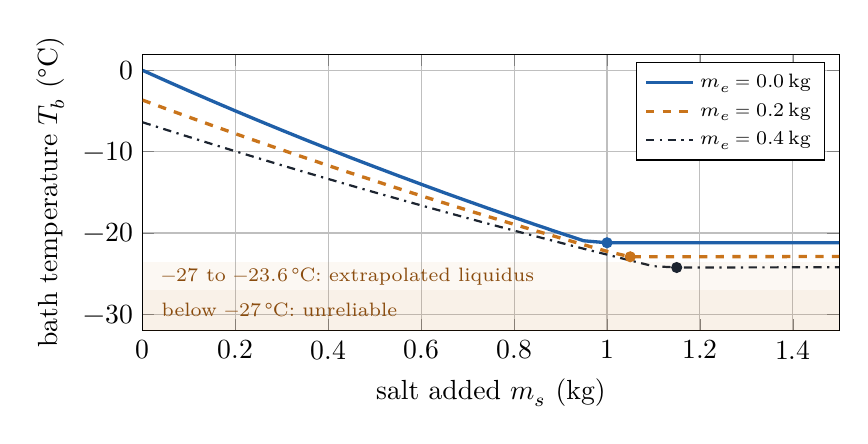
\begin{tikzpicture}
\begin{axis}[width=0.86\linewidth, height=0.42\linewidth, xlabel={salt added $m_s$ (kg)}, ylabel={bath temperature $T_b$ (\textdegree C)},
  xmin=0, xmax=1.5, ymin=-32, ymax=2, grid=major, legend cell align=left, legend style={font=\scriptsize, at={(0.98,0.97)}, anchor=north east}]
\addplot[cBlue, very thick] coordinates {(0,-0) (0.05,-1.28) (0.1,-2.54) (0.15,-3.777) (0.2,-4.994) (0.25,-6.19) (0.3,-7.366) (0.35,-8.522) (0.4,-9.658) (0.45,-10.78) (0.5,-11.87) (0.55,-12.95) (0.6,-14.01) (0.65,-15.06) (0.7,-16.08) (0.75,-17.09) (0.8,-18.08) (0.85,-19.06) (0.9,-20.02) (0.95,-20.96) (1,-21.2) (1.05,-21.2) (1.1,-21.2) (1.15,-21.2) (1.2,-21.2) (1.25,-21.2) (1.3,-21.2) (1.35,-21.2) (1.4,-21.2) (1.45,-21.2) (1.5,-21.2)};
\addlegendentry{$m_e=0.0$\,kg}
\addplot[only marks, mark=*, mark size=1.8pt, forget plot, cBlue] coordinates {(1.000,-21.200)};
\addplot[cAmber, very thick, dashed] coordinates {(0,-3.662) (0.05,-4.715) (0.1,-5.755) (0.15,-6.781) (0.2,-7.794) (0.25,-8.794) (0.3,-9.78) (0.35,-10.75) (0.4,-11.71) (0.45,-12.66) (0.5,-13.59) (0.55,-14.52) (0.6,-15.43) (0.65,-16.32) (0.7,-17.21) (0.75,-18.08) (0.8,-18.94) (0.85,-19.79) (0.9,-20.62) (0.95,-21.45) (1,-22.26) (1.05,-22.93) (1.1,-22.92) (1.15,-22.92) (1.2,-22.92) (1.25,-22.91) (1.3,-22.91) (1.35,-22.91) (1.4,-22.9) (1.45,-22.9) (1.5,-22.9)};
\addlegendentry{$m_e=0.2$\,kg}
\addplot[only marks, mark=*, mark size=1.8pt, forget plot, cAmber] coordinates {(1.050,-22.926)};
\addplot[cInk, thick, dashdotted] coordinates {(0,-6.389) (0.05,-7.295) (0.1,-8.192) (0.15,-9.079) (0.2,-9.955) (0.25,-10.82) (0.3,-11.68) (0.35,-12.53) (0.4,-13.36) (0.45,-14.19) (0.5,-15.01) (0.55,-15.81) (0.6,-16.61) (0.65,-17.4) (0.7,-18.18) (0.75,-18.95) (0.8,-19.71) (0.85,-20.46) (0.9,-21.2) (0.95,-21.94) (1,-22.66) (1.05,-23.38) (1.1,-24.09) (1.15,-24.24) (1.2,-24.24) (1.25,-24.24) (1.3,-24.23) (1.35,-24.23) (1.4,-24.22) (1.45,-24.22) (1.5,-24.21)};
\addlegendentry{$m_e=0.4$\,kg}
\addplot[only marks, mark=*, mark size=1.8pt, forget plot, cInk] coordinates {(1.150,-24.245)};
\fill[cAmber, opacity=0.10] (axis cs:0,-27) rectangle (axis cs:1.5,-32);
\fill[cAmber, opacity=0.05] (axis cs:0,-23.6) rectangle (axis cs:1.5,-27);
\node[font=\scriptsize, anchor=west, cAmberDark] at (axis cs:0.02,-29.5) {below $-27$\,\textdegree C: unreliable};
\node[font=\scriptsize, anchor=west, cAmberDark] at (axis cs:0.02,-25.3) {$-27$ to $-23.6$\,\textdegree C: extrapolated liquidus};
\end{axis}
\end{tikzpicture}
\caption{Bath temperature against salt for three ethanol loadings ($m_w=1.6$, $m_i=4.0$\,kg). The dot marks where the brine saturates. With salt only, the curve then stays flat at the eutectic: it is a thermostat. With ethanol it keeps sinking slowly along the cotectic. Shading marks where the liquidus data run out.}
\label{fig:tbsalt}
\end{figure}

\begin{figure}[H]
\centering

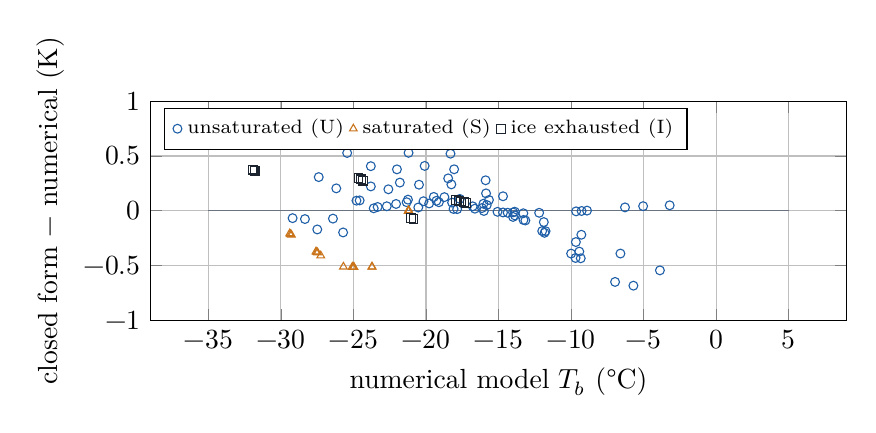
\begin{tikzpicture}
\begin{axis}[width=0.86\linewidth, height=0.36\linewidth, xlabel={numerical model $T_b$ (\textdegree C)}, ylabel={closed form $-$ numerical (K)},
  ymin=-1, ymax=1, grid=major, legend cell align=left, legend style={font=\scriptsize, at={(0.02,0.97)}, anchor=north west}, legend columns=3]
\addplot[only marks, mark size=1.6pt, mark=o, cBlue] coordinates {(-9.334,-0.4335) (-14.69,0.1323) (-18.31,0.5209) (-20.94,0.7296) (-8.902,0.001509) (-14.69,-0.01553) (-18.47,0.2956) (-21.2,0.5287) (-23.29,0.6702) (-16.01,-0.001789) (-19.28,0.09077) (-21.8,0.2573) (-23.8,0.4069) (-25.43,0.5274) (-23.33,0.0347) (-24.79,0.09231) (-26.18,0.2044) (-27.39,0.3073) (-27.49,-0.1704) (-28.34,-0.07555) (-29.19,-0.06736) (-5.705,-0.6835) (-9.997,-0.3908) (-13.29,-0.02269) (-15.89,0.2782) (-5.036,0.04204) (-9.67,-0.2854) (-13.15,-0.08855) (-15.86,0.1587) (-18.06,0.3786) (-9.653,-0.005226) (-13.28,-0.08391) (-16.04,0.06423) (-18.25,0.2407) (-20.09,0.4094) (-14,-0.01492) (-16.63,0.01897) (-18.73,0.1245) (-20.48,0.2379) (-22,0.378) (-18.1,0.01635) (-19.78,0.06669) (-21.24,0.1014) (-22.59,0.196) (-23.8,0.2224) (-22.7,0.04131) (-23.6,0.0225) (-24.57,0.09443) (-25.71,-0.1978) (-26.41,-0.07166) (-3.879,-0.5438) (-6.969,-0.6493) (-9.691,-0.4308) (-11.99,-0.185) (-3.205,0.04989) (-6.599,-0.3903) (-9.432,-0.3725) (-11.83,-0.2012) (-13.88,-0.008858) (-6.284,0.03089) (-9.292,-0.2188) (-11.76,-0.1858) (-13.87,-0.04289) (-15.66,0.0987) (-9.276,-0.001994) (-11.88,-0.1033) (-14,-0.05611) (-15.81,0.05267) (-12.2,-0.01843) (-14.37,-0.01812) (-16.14,0.02479) (-17.67,0.1082) (-15.07,-0.009441) (-16.78,0.04068) (-18.2,0.07481) (-19.46,0.1264) (-17.85,0.01493) (-19.11,0.07791) (-20.17,0.08691) (-20.53,0.02994) (-21.33,0.07823) (-22.06,0.06204)};
\addlegendentry{unsaturated (U)}
\addplot[only marks, mark size=1.6pt, mark=triangle, cAmber] coordinates {(-21.2,0) (-21.2,0) (-25.08,-0.5131) (-21.2,0) (-25.04,-0.5136) (-27.58,-0.3735) (-29.39,-0.2082) (-21.2,0) (-25,-0.514) (-27.52,-0.3776) (-29.33,-0.2146) (-21.2,0) (-24.96,-0.5145) (-27.47,-0.3817) (-29.27,-0.2209) (-21.2,0) (-21.2,0) (-23.73,-0.5123) (-21.2,0) (-23.71,-0.5114) (-25.69,-0.5113) (-27.25,-0.4093)};
\addlegendentry{saturated (S)}
\addplot[only marks, mark size=1.6pt, mark=square, cInk] coordinates {(-31.81,0.3611) (-31.95,0.3758) (-24.34,0.276) (-24.5,0.2864) (-24.65,0.2969) (-17.23,0.07048) (-17.4,0.07743) (-17.57,0.08443) (-20.86,-0.07466) (-17.74,0.09149) (-21.02,-0.06574) (-17.91,0.0986)};
\addlegendentry{ice exhausted (I)}
\addplot[cGrey, thin, forget plot] coordinates {(-35,0) (5,0)};
\end{axis}
\end{tikzpicture}
\caption{Closed form minus numerical model for \val{BathN} recipes, by regime.}
\label{fig:bathval}
\end{figure}

% =====================================================================================================
\section{Part II \,\textperiodcentered\, The can, its air space, and where things sit in the tank}\label{sec:geom}

\subsection{The part-filled can}\label{sec:can}
Treat the can as a cylinder of outer radius $R$ and height $H$, with a wall of thickness $t_w$. The drink of volume $V_d$ stands at the bottom; above it is the air space (headspace gas).
\begin{equation}
r_i=R-t_w,\qquad h_d=\frac{V_d}{\pi r_i^2},\qquad V_a=\pi r_i^2H-V_d,\qquad h_a=H-h_d,
\label{eq:can}
\end{equation}
\begin{equation}
C=\rho_dV_dc_d+m_{\rm Al}c_{\rm Al},\qquad M_c=\rho_dV_d+m_{\rm Al},\qquad \bar\rho_c=\frac{M_c}{\pi R^2H}.
\label{eq:canC}
\end{equation}
$h_d$ is the height of the drink column, $V_a$ and $h_a$ the volume and height of the air space, $C$ the heat capacity that has to be cooled (drink plus aluminium), $M_c$ the can's mass and $\bar\rho_c$ its mean density.

\begin{center}\footnotesize
\begin{tabular}{@{}l r r l@{}}
\toprule
 & Can 2 (standard) & Can 1 (slim) & \\
\midrule
outer diameter, height & \val{Ctwod}, \val{CtwoH}\,mm & \val{Coned}, \val{ConeH}\,mm & measured \\
drink column $h_d$ (330\,mL) & \val{Ctwohd}\,mm & \val{Conehd}\,mm & Eq.~\eqref{eq:can} \\
air space $V_a$ (share of the inside), height $h_a$ & \val{CtwoVa}\,mL (\val{Ctwoair}\,\%), \val{Ctwoha}\,mm & \val{ConeVa}\,mL (\val{Coneair}\,\%), \val{Coneha}\,mm & Eq.~\eqref{eq:can} \\
heat capacity $C$ & \val{CtwoC}\,J/K & \val{ConeC}\,J/K & Eq.~\eqref{eq:canC} \\
mass $M_c$, mean density $\bar\rho_c$ & \val{CtwoMc}\,g, \val{Ctworho}\,kg/m$^3$ & \val{ConeMc}\,g, \val{Conerho}\,kg/m$^3$ & Eq.~\eqref{eq:canC} \\
free-floating draft in eutectic brine / in water & \val{Ctwodfb} / \val{Ctwodfw}\,mm & \val{Conedfb} / \val{Conedfw}\,mm & Eq.~\eqref{eq:buoy} \\
force to hold it fully under eutectic brine & \val{CtwoF}\,N & \val{ConeF}\,N & Eq.~\eqref{eq:buoy} \\
\bottomrule
\end{tabular}
\end{center}

The air space does three separate things, and each enters the model in a different place:
\begin{enumerate}
\item it \textbf{lowers the heat capacity}: only the drink and the can need cooling (Eq.~\eqref{eq:canC});
\item it \textbf{leaves a dry band of wall} at the top. Inside that band is gas, so the drink can only reach it by conduction along the aluminium. That band acts as a cooling fin (\S\ref{sec:zones});
\item it \textbf{makes the can float}: $\bar\rho_c<\rho_b$, and here even $\bar\rho_c<1000$\,kg/m$^3$.
\end{enumerate}

\subsection{Buoyancy}\label{sec:buoy}
A free can floats upright with draft $d_f$. To hold it at an immersion depth $h_o$ you have to push it down with a force $F$:
\begin{equation}
d_f=\frac{M_c}{\rho_b\,\pi R^2},\qquad F=\rho_b\,g\,\pi R^2h_o-M_cg .
\label{eq:buoy}
\end{equation}
A 330\,mL can floats even in fresh water: its draft there is \val{Ctwodfw}\,mm of its \val{CtwoH}\,mm. In eutectic brine its waterline sits at \val{Ctwodfb}\,mm, so the top \val{Ctwoexp}\,mm of the drink column would stick out, and it needs \val{CtwoF}\,N to hold it fully under. So it must be clamped, and the lid board in your rig note does exactly that. A floating can is also barely stable upright. Its centre of mass (near the middle of the drink) sits at about the height of its metacentre, so left alone it tips over.

\subsection{Where the ice and the brine end up}\label{sec:layers}
From Part I take the ice left $m_I=m_i-x$, the brine mass $m_b=W+n_dM_s+n_e'M_e$, the brine density $\rho_b=\rho_0+\beta_sw_s-\beta_ew_e$ (with $w_s$, $w_e$ the salt and ethanol mass fractions), and any solid salt $m_{ss}$. Then
\begin{equation}
V_I=\frac{m_I}{\rho_i},\quad V_b=\frac{m_b}{\rho_b}+\frac{m_{ss}}{\rho_{\rm NaCl}},\quad A'=A_t-\pi R^2,\quad h_p=\frac{V_I}{\varphi_pA'},\quad V_p=\frac{1-\varphi_p}{\varphi_p}\,V_I .
\label{eq:vols}
\end{equation}
$A'$ is the floor area beside the can, $h_p$ the height the ice pack would occupy, and $V_p$ the brine needed to fill all its pores. Ice is lighter than brine, so the layering depends on how you hold the ice (Fig.~\ref{fig:tank}):
\begin{itemize}
\item \textbf{Ice floats freely.} By Archimedes a fraction $\rho_i/\rho_b$ of the pack is under the surface, holding $V_f=(\rho_i/\rho_b)V_p$ of brine in its pores. The rest of the brine sits under the ice as a clear layer:
\begin{equation}
h_{cb}=\frac{V_b-V_f}{A'},\qquad h_b=h_{cb}+\frac{\rho_i}{\rho_b}\,h_p,\qquad \text{ice above the surface: }\Big(1-\frac{\rho_i}{\rho_b}\Big)h_p .
\label{eq:float}
\end{equation}
\item \textbf{Ice pushed under a lid board.} The whole pack is submerged: $h_{cb}=(V_b-V_p)/A'$, and slush runs from $h_{cb}$ up to $h_b=h_{cb}+h_p$.
\item \textbf{Ice held down at the floor} (a mesh). Slush runs from the floor up to $h_p$, with clear brine above it up to $h_b=h_p+(V_b-V_p)/A'$.
\end{itemize}
If there is too little brine to float or submerge the pack ($V_b<V_f$, or $V_b<V_p$), the ice rests on the floor. Then $h_b=V_b/[(1-\varphi_p)A']$, slush runs from the floor to $h_b$, and dry ice sits above. Plain ice water B0 is like this. Finally, everything must fit: the top of the pack must stay below $H_t$.

\begin{center}\footnotesize
\begin{tabular}{@{}l l r r r r r l@{}}
\toprule
recipe & ice held & clear brine $h_{cb}$ & surface $h_b$ & pack top & slush on can $L_{sl}$ & brine on can $L_{br}$ & fits? \\
\midrule
B1 & floats & \val{B1Flhcb} & \val{B1Flhb} & \val{B1Flhtop} & \val{B1FlLsl} & \val{B1FlLbr} & at brim \\
B1 & lid board & \val{B1Bdhcb} & \val{B1Bdhb} & \val{B1Bdhtop} & \val{B1BdLsl} & \val{B1BdLbr} & \val{B1Bdfits} \\
B1 & at floor & 0 & \val{B1Fohb} & \val{B1Fohtop} & \val{B1FoLsl} & \val{B1FoLbr} & \val{B1Fofits} \\
B3 & lid board & \val{B3Bdhcb} & \val{B3Bdhb} & \val{B3Bdhtop} & \val{B3BdLsl} & \val{B3BdLbr} & \val{B3Bdfits} \\
B4 & lid board & \val{B4Bdhcb} & \val{B4Bdhb} & \val{B4Bdhtop} & \val{B4BdLsl} & \val{B4BdLbr} & \val{B4Bdfits} \\
B4 & at floor & 0 & \val{B4Fohb} & \val{B4Fohtop} & \val{B4FoLsl} & \val{B4FoLbr} & \val{B4Fofits} \\
\bottomrule
\end{tabular}\\[0.2em]
{\scriptsize All heights and lengths in cm, measured from the tank floor; the can's base is at $z_0=\val{zzero}$\,cm.}
\end{center}
B4 (your original charge) melts so much ice that with the lid board most of the drink column sits in clear brine: only \val{B4BdLsl}\,cm of the \val{Ctwohdcm}\,cm drink column touches slush. That matters a lot in \S\ref{sec:heat}.

\subsection{Contact zones on the can}\label{sec:zones}
The drink wets the wall from $z_0$ to $z_0+h_d$. Overlapping that band with each layer gives the lengths of wall that have drink inside and slush, or clear brine, outside ($L_{sl}$, $L_{br}$). Wall facing ice above the brine surface, or air, is treated as insulated (A8). The bottom counts if the can is held off the floor ($z_0>0$).
\begin{equation}
A_{sl}=2\pi R\,L_{sl},\qquad A_{br}=2\pi R\,L_{br},\qquad A_{\rm bot}=\pi R^2 .
\label{eq:areas}
\end{equation}
\textbf{The dry band as a fin.} Above the drink line the wall has gas inside and liquid outside. It still cools the drink, because heat runs along the aluminium from the wetted wall. A thin fin of conductance $k_{\rm Al}t_w$ per unit width, losing heat to the outside with a mean coefficient $\bar h$, carries heat only over a length $1/m$:
\begin{equation}
m=\sqrt{\frac{\bar h}{k_{\rm Al}t_w}},\qquad A_{\rm fin}=2\pi R\,\frac{\tanh(mL_f)}{m},\qquad
A_{[x_a,x_b]}=2\pi R\,\frac{\sinh m(L_f-x_a)-\sinh m(L_f-x_b)}{m\cosh mL_f}.
\label{eq:fin}
\end{equation}
$L_f$ is the length of dry wall in liquid. The last expression splits $A_{\rm fin}$ between layers when the band crosses from slush into brine. With $\bar h\approx\val{B1Fohbar}$\,W\,m$^{-2}$K$^{-1}$ (from \S\ref{sec:heat}), $1/m\approx9$\,mm. So only the first centimetre of the \val{Ctwoha}\,mm dry band works, contributing $A_{\rm fin}\approx\val{B1FoAfin}$\,cm$^2$ of the \val{B1FoAtot}\,cm$^2$ total contact area for B1 with the ice at the floor. $\bar h$ comes from the first pass of the cooling calculation, so the fin enters on the second pass.

% =====================================================================================================
\section{Part III \,\textperiodcentered\, Heat flow with no convection}\label{sec:heat}

\begin{plain}[The story in four steps]
\begin{enumerate}[leftmargin=1.3em]
\item With nothing flowing, the salt next to the can cannot follow the meltwater. The brine there gets diluted, and the last ice beside the can melts at $T_L$, well above $T_b$ (\S\ref{sec:etac}).
\item The slush does not melt at one temperature. Its latent heat is spread over a partly melted zone, so it behaves like a solid with a huge, temperature-dependent heat capacity (\S\ref{sec:mushy}).
\item A classical similarity solution turns that zone into one number, an effective \emph{effusivity} $E$ (\S\ref{sec:neumann}).
\item A well-mixed can in contact with such a material cools by an exact closed-form law, which comes out of a Laplace transform (\S\ref{sec:law}).
\end{enumerate}
\end{plain}

\subsection{What ``no convection'' does}\label{sec:noconv}
Heat then moves only by conduction, $\partial H/\partial t=\nabla\!\cdot(k\nabla T)$ with $H$ the enthalpy per unit volume, in the drink, the wall, the brine and the slush. The second consequence is easy to miss: \textbf{dissolved salt and ethanol stay put}. They could only move by diffusion, with $D\approx1.5\times10^{-9}$\,m$^2$/s, while heat diffuses with $\alpha\approx1.3\times10^{-7}$\,m$^2$/s. The ratio (the Lewis number) is about 90. In a 200\,s cooling, salt moves about $\sqrt{Dt}\approx0.5$\,mm while heat reaches about 5\,mm. So the water from ice melted by the can stays where it melted.

\subsection{The diluted brine at the can: the coefficient you asked for}\label{sec:etac}
Take one cubic metre of slush next to the can, with ice volume fraction $\varphi_p$ and its pores full of bath brine (mass fractions $w_w,w_s,w_e$):
\begin{equation}
W_0=(1-\varphi_p)\rho_bw_w,\quad m_{I0}=\varphi_p\rho_i,\quad n_{s,v}=\frac{(1-\varphi_p)\rho_bw_s}{M_s},\quad n_{e,v}=\frac{(1-\varphi_p)\rho_bw_e}{M_e},
\label{eq:slush}
\end{equation}
with $N_v=K_sn_{s,v}+K_en_{e,v}$ and $W_{b,v}=\omega_sn_{s,v}+\omega_en_{e,v}$. Because the solutes cannot leave, Eq.~\eqref{eq:liq} applies to this cubic metre with its own fixed $N_v$. At depression $\theta$ it holds liquid water $W_l(\theta)=W_{b,v}+N_v/\theta$ and ice $m_I(\theta)=W_0+m_{I0}-W_l(\theta)$. Far away it sits at $\theta_b$ with $W_l=W_0$. Heated, it melts progressively, and the last ice goes when $W_l=W_0+m_{I0}$:
\begin{equation}
\theta_L=\frac{N_v}{W_0+m_{I0}-W_{b,v}},\qquad
\boxed{\;\eta_c\equiv\frac{\theta_L}{\theta_b}=\frac{W_0-W_{b,v}}{W_0+m_{I0}-W_{b,v}}\;}
\label{eq:etac}
\end{equation}
$\eta_c$ is the ratio of free water in the brine alone to free water in brine plus ice. It is a ``lowered coefficient'' that needs no fitting: it follows from the no-convection assumption and the ice fraction. For B1 ($W_0=\val{SlWzero}$, $m_{I0}=\val{SlmIzero}$, $W_{b,v}=\val{SlWb}$\,kg/m$^3$), $\eta_c=\val{SlEtac}$. The last ice next to the can therefore melts at $T_L=\val{SlTL}$\,\textdegree C, while the bath a few centimetres away is at $-21.2$\,\textdegree C.

\begin{warn}[Two different coefficients, both lowered]
Your mixing coefficient $\eta_s$ (\S\ref{sec:eta}) describes the \emph{whole bath}: how much of the salt you poured actually dissolved. It sets $T_b$. The no-convection coefficient $\eta_c$ describes the \emph{few millimetres next to the can}: how much the can's own meltwater dilutes the brine there. They multiply: $\theta_L=\eta_c\,\theta_b(\eta_s)$. If undissolved salt crystals sit in the slush right against the can, $\eta_c$ moves towards 1, because melting can then stay at the eutectic until the local crystals run out.
\end{warn}

\subsection{The slush is a heat sink with its latent heat spread out}\label{sec:mushy}
Per unit volume, measuring from all-liquid at 0\,\textdegree C, the enthalpy of the slush is
\begin{equation}
H(\theta)=-m_I(\theta)\,(L_0-\Delta c\,\theta)-\theta\,C_v,\qquad C_v=c_w(W_0+m_{I0})+c_sM_sn_{s,v}+c_{ea}M_en_{e,v}.
\label{eq:H}
\end{equation}
Its slope with temperature, the \emph{apparent heat capacity}, is
\[
c_{\rm app}=\frac{\dd H}{\dd T}=C_v-\Delta c\,m_I(\theta)+(L_0-\Delta c\,\theta)\frac{N_v}{\theta^2}\qquad(\theta_L<\theta<\theta_b),\qquad c_{\rm app}=C_v\quad(\theta<\theta_L).
\]
Three features matter.
\begin{itemize}
\item There is \textbf{no latent-heat jump} at $T_L$: the ice fraction falls continuously to zero there.
\item Most of the latent heat is taken up near $T_L$, because $N_v/\theta^2$ is largest there.
\item The total heat needed to turn slush at $T_b$ into liquid at $T_L$ is
\end{itemize}
\begin{equation}
\Delta H=m_{I0}\,(L_0-\Delta c\,\theta_b)+C_v\,(\theta_b-\theta_L)\qquad(\text{B1: }\val{SldH}\,\text{MJ/m}^3,\ C_v=\val{SlCv}\,\text{MJ\,m}^{-3}\text{K}^{-1}).
\label{eq:dH}
\end{equation}
The numerical solution of the full conduction problem (Fig.~\ref{fig:profiles}) shows what this does. Behind the full-melt isotherm there is only a thin liquid layer: \val{Heat240L}\,mm after 240\,s. Ahead of it a broad, partly melted zone reaches 1--2\,cm, and it holds \val{Heat60pc}\,\% of the heat taken from the can after 60\,s and \val{Heat240pc}\,\% after 240\,s. A sharp-front (Stefan) model that puts all the latent heat at $T_L$ ignores that zone, and comes out too slow: by \val{StMidErr}\,\% at $\theta_b\approx5$\,K and by \val{StEutErr}\,\% at the eutectic (Appendix~\ref{sec:stefan}).

\begin{figure}[H]
\centering

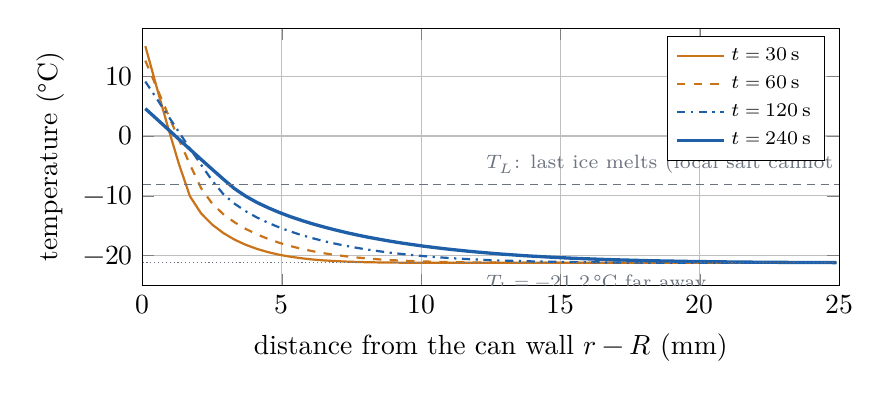
\begin{tikzpicture}
\begin{axis}[width=0.86\linewidth, height=0.40\linewidth, xlabel={distance from the can wall $r-R$ (mm)}, ylabel={temperature (\textdegree C)},
  xmin=0, xmax=25, ymin=-25, ymax=18, grid=major, legend cell align=left, legend style={font=\scriptsize, at={(0.98,0.97)}, anchor=north east}]
\addplot[cAmber, thick] coordinates {(0.1,15.01) (0.5,8.266) (0.9,1.657) (1.3,-4.613) (1.7,-10.07) (2.1,-12.93) (2.5,-14.81) (2.9,-16.22) (3.3,-17.32) (3.7,-18.18) (4.1,-18.86) (4.5,-19.41) (4.9,-19.84) (5.3,-20.17) (5.7,-20.43) (6.1,-20.64) (6.5,-20.79) (6.9,-20.9) (7.3,-20.99) (7.7,-21.05) (8.1,-21.1) (8.5,-21.13) (8.9,-21.15) (9.3,-21.17) (9.7,-21.18) (10.1,-21.19) (10.5,-21.19) (10.9,-21.2) (11.3,-21.2) (11.7,-21.2) (12.1,-21.2) (12.5,-21.2) (12.9,-21.2) (13.3,-21.2) (13.7,-21.2) (14.1,-21.2) (14.5,-21.2) (14.9,-21.2) (15.3,-21.2) (15.7,-21.2) (16.1,-21.2) (16.5,-21.2) (16.9,-21.2) (17.3,-21.2) (17.7,-21.2) (18.1,-21.2) (18.5,-21.2) (18.9,-21.2) (19.3,-21.2) (19.7,-21.2) (20.1,-21.2) (20.5,-21.2) (20.9,-21.2) (21.3,-21.2) (21.7,-21.2) (22.1,-21.2) (22.5,-21.2) (22.9,-21.2) (23.3,-21.2) (23.7,-21.2) (24.1,-21.2) (24.5,-21.2) (24.9,-21.2)};
\addlegendentry{$t=30$\,s}
\addplot[cAmber, thick, dashed] coordinates {(0.1,12.58) (0.5,8.166) (0.9,3.771) (1.3,-0.5515) (1.7,-4.757) (2.1,-8.718) (2.5,-11.31) (2.9,-13.07) (3.3,-14.42) (3.7,-15.52) (4.1,-16.43) (4.5,-17.19) (4.9,-17.84) (5.3,-18.39) (5.7,-18.85) (6.1,-19.25) (6.5,-19.59) (6.9,-19.87) (7.3,-20.11) (7.7,-20.31) (8.1,-20.48) (8.5,-20.62) (8.9,-20.74) (9.3,-20.83) (9.7,-20.91) (10.1,-20.97) (10.5,-21.02) (10.9,-21.06) (11.3,-21.09) (11.7,-21.12) (12.1,-21.14) (12.5,-21.15) (12.9,-21.17) (13.3,-21.17) (13.7,-21.18) (14.1,-21.19) (14.5,-21.19) (14.9,-21.19) (15.3,-21.19) (15.7,-21.2) (16.1,-21.2) (16.5,-21.2) (16.9,-21.2) (17.3,-21.2) (17.7,-21.2) (18.1,-21.2) (18.5,-21.2) (18.9,-21.2) (19.3,-21.2) (19.7,-21.2) (20.1,-21.2) (20.5,-21.2) (20.9,-21.2) (21.3,-21.2) (21.7,-21.2) (22.1,-21.2) (22.5,-21.2) (22.9,-21.2) (23.3,-21.2) (23.7,-21.2) (24.1,-21.2) (24.5,-21.2) (24.9,-21.2)};
\addlegendentry{$t=60$\,s}
\addplot[cBlue, thick, dashdotted] coordinates {(0.1,9.093) (0.5,6.287) (0.9,3.477) (1.3,0.6802) (1.7,-2.085) (2.1,-4.802) (2.5,-7.456) (2.9,-9.725) (3.3,-11.32) (3.7,-12.57) (4.1,-13.61) (4.5,-14.5) (4.9,-15.27) (5.3,-15.95) (5.7,-16.55) (6.1,-17.08) (6.5,-17.56) (6.9,-17.98) (7.3,-18.36) (7.7,-18.7) (8.1,-19) (8.5,-19.27) (8.9,-19.51) (9.3,-19.72) (9.7,-19.91) (10.1,-20.08) (10.5,-20.23) (10.9,-20.36) (11.3,-20.48) (11.7,-20.58) (12.1,-20.67) (12.5,-20.75) (12.9,-20.81) (13.3,-20.87) (13.7,-20.92) (14.1,-20.97) (14.5,-21) (14.9,-21.04) (15.3,-21.06) (15.7,-21.09) (16.1,-21.11) (16.5,-21.12) (16.9,-21.14) (17.3,-21.15) (17.7,-21.16) (18.1,-21.17) (18.5,-21.17) (18.9,-21.18) (19.3,-21.18) (19.7,-21.19) (20.1,-21.19) (20.5,-21.19) (20.9,-21.19) (21.3,-21.19) (21.7,-21.2) (22.1,-21.2) (22.5,-21.2) (22.9,-21.2) (23.3,-21.2) (23.7,-21.2) (24.1,-21.2) (24.5,-21.2) (24.9,-21.2)};
\addlegendentry{$t=120$\,s}
\addplot[cBlue, very thick] coordinates {(0.1,4.563) (0.5,2.873) (0.9,1.175) (1.3,-0.5264) (1.7,-2.223) (2.1,-3.909) (2.5,-5.578) (2.9,-7.224) (3.3,-8.802) (3.7,-10.06) (4.1,-11.1) (4.5,-11.98) (4.9,-12.77) (5.3,-13.47) (5.7,-14.1) (6.1,-14.68) (6.5,-15.2) (6.9,-15.68) (7.3,-16.13) (7.7,-16.54) (8.1,-16.92) (8.5,-17.26) (8.9,-17.59) (9.3,-17.89) (9.7,-18.16) (10.1,-18.42) (10.5,-18.65) (10.9,-18.87) (11.3,-19.07) (11.7,-19.26) (12.1,-19.43) (12.5,-19.59) (12.9,-19.74) (13.3,-19.87) (13.7,-20) (14.1,-20.11) (14.5,-20.21) (14.9,-20.31) (15.3,-20.4) (15.7,-20.48) (16.1,-20.55) (16.5,-20.62) (16.9,-20.68) (17.3,-20.73) (17.7,-20.78) (18.1,-20.83) (18.5,-20.87) (18.9,-20.9) (19.3,-20.94) (19.7,-20.97) (20.1,-20.99) (20.5,-21.02) (20.9,-21.04) (21.3,-21.06) (21.7,-21.08) (22.1,-21.09) (22.5,-21.1) (22.9,-21.12) (23.3,-21.13) (23.7,-21.14) (24.1,-21.14) (24.5,-21.15) (24.9,-21.16)};
\addlegendentry{$t=240$\,s}
\addplot[cGrey, densely dashed, forget plot] coordinates {(0,-8.143) (25,-8.143)};
\addplot[cGrey, densely dotted, forget plot] coordinates {(0,-21.2) (25,-21.2)};
\node[font=\scriptsize, anchor=south west, cGrey] at (axis cs:12,-7.84) {$T_L$: last ice melts (local salt cannot move)};
\node[font=\scriptsize, anchor=north west, cGrey] at (axis cs:12,-21.5) {$T_b=-21.2$\,\textdegree C far away};
\end{axis}
\end{tikzpicture}
\caption{Temperature around a well-mixed Can 2 in B1 slush ($\varphi_p=\val{phip}$), from the numerical solution of the conduction problem. Left of the dashed line $T_L$ the slush has fully melted (a few mm). To the right, a broad partly melted zone at temperatures between $T_L$ and $T_b$ soaks up nearly half of the heat.}
\label{fig:profiles}
\end{figure}

\subsection{One number for the slush: its effective effusivity}\label{sec:neumann}
\textbf{The classical problem.} Hold a flat wall at temperature $T_w$ against a half-space of slush at $T_b$. With no length scale in the problem, the solution depends only on $\xi/\sqrt t$ ($\xi$ is the distance from the wall). Treat the liquid layer (conductivity $k_l$, heat capacity $C_v$, diffusivity $\alpha_l=k_l/C_v$) and the partly melted zone separately. Give the second constant effective properties: $c_m=\Delta H/(\theta_b-\theta_L)$, and $k_m$ = the mean slush conductivity between $T_b$ and $T_L$ (ice fraction weighted, Maxwell--Eucken), with $\alpha_m=k_m/c_m$. The isotherm $T_L$ then moves as $s=2\lambda\sqrt{\alpha_lt}$ and
\[
T=T_w-(T_w-T_L)\frac{\erf\big(\xi/2\sqrt{\alpha_lt}\big)}{\erf\lambda}\ (\xi<s),\qquad
T=T_b+(T_L-T_b)\frac{\erfc\big(\xi/2\sqrt{\alpha_mt}\big)}{\erfc\big(\lambda\sqrt{\alpha_l/\alpha_m}\big)}\ (\xi>s).
\]
There is no latent jump at $T_L$, so the heat flux must be continuous there. That fixes $\lambda$:
\begin{equation}
\frac{E_l\,(T_w-T_L)\,e^{-\lambda^2}}{\erf\lambda}=\frac{E_m\,(T_L-T_b)\,e^{-\lambda^2\alpha_l/\alpha_m}}{\erfc\!\big(\lambda\sqrt{\alpha_l/\alpha_m}\big)},\qquad E_l=\sqrt{k_lC_v},\quad E_m=\sqrt{k_mc_m}.
\label{eq:neumann}
\end{equation}
This is one equation in one unknown, solved once (B1: $\lambda=\val{B1Folam}$). The flux through the wall is then
\begin{equation}
q=\frac{E_l(T_w-T_L)}{\erf\lambda\,\sqrt{\pi t}}\equiv\frac{E\,(T_w-T_b)}{\sqrt{\pi t}},\qquad
\boxed{\;E=\frac{E_l\,(T_w-T_L)}{(T_w-T_b)\,\erf\lambda}\;}
\label{eq:E}
\end{equation}
$E$ is exactly what a uniform material of effusivity $E$ would give. So, as far as the wall can tell, the slush behaves like such a material, with an effective conductivity and heat capacity
\begin{equation}
k=\frac{E^2}{c_{\rm sec}},\qquad c_{\rm sec}=\frac{\Delta H+C_v(T_w-T_L)}{T_w-T_b}.
\label{eq:keff}
\end{equation}
For B1: $E_l=\val{SlEl}$, $E_m=\val{SlEm}$ and $E=\val{B1FoEs}$\,W\,s$^{1/2}$\,m$^{-2}$\,K$^{-1}$, with $k=\val{B1Foks}$\,W\,m$^{-1}$K$^{-1}$. In plain ice water ($\theta_b=0$) the ice melts at one temperature, so Eq.~\eqref{eq:neumann} becomes the textbook one-phase Stefan condition $\lambda e^{\lambda^2}\erf\lambda=\mathrm{Ste}/\sqrt\pi$, with $\mathrm{Ste}=C_vT_w/(m_{I0}L_0)$.

\textbf{Which wall temperature?} The drink cools, so $T_w$ falls from $T_0$ to $T_1$ and $E$ changes along the way. Two limits fix the choice. When the partly melted range $\theta_b-\theta_L$ is wide compared with how far the drink ends above $T_L$, the slush behaves almost linearly and the time-averaged drink temperature $\bar T$ is right. When that range is narrow (fresh water), the slush behaves like a sharp front, the last stage dominates, and $T_1$ is right. Interpolating between them,
\begin{equation}
T_{\rm ref}=w\,\bar T+(1-w)\,T_1,\qquad w=\min(1,\psi),\qquad \psi=\frac{\theta_b-\theta_L}{T_1-T_L},
\label{eq:Tref}
\end{equation}
with $\bar T$ from Eq.~\eqref{eq:Tbar} below (two or three passes converge). B1 has $\psi=\val{B1Bdpsi}$, so $T_{\rm ref}=\val{B1BdTref}$\,\textdegree C. Plain ice water has $\psi=0$, so $T_{\rm ref}=T_1$. This rule is the only empirical step in Part III. Without it, the error against the full solution rises from \val{PdeMax}\,\% to about 50\,\% for nearly fresh baths.

\subsection{The cooling law}\label{sec:law}
\textbf{Set-up.} Let $\Theta(t)=T_d(t)-T_b$ be the drink's excess over the bath. A well-mixed drink loses heat through its contact area $A$:
\[
C\,\frac{\dd\Theta}{\dd t}=-A\,q(t).
\]
For a medium of effusivity $E$ and conductivity $k$ around a cylinder of radius $R$, the response to a wall excess $\Theta_w(t)$ is, in Laplace variables ($\hat f(s)=\int_0^\infty f e^{-st}\dd t$),
\[
\hat q(s)=\Big(E\sqrt s+\frac{k}{2R}\Big)\hat\Theta_w(s).
\]
The first term is the flat-wall response, $q=E\Theta_w/\sqrt{\pi t}$ for a step. The second is the first correction for the curved surface (for a step it adds the steady $k\Theta_w/2R$). The aluminium has no resistance and the drink is well mixed, so $\Theta_w=\Theta$. Transforming the drink equation, with $\Theta(0)=\Theta_0$:
\[
C\big(s\hat\Theta-\Theta_0\big)=-A\Big(E\sqrt s+\frac{k}{2R}\Big)\hat\Theta
\quad\Longrightarrow\quad
\hat\Theta=\frac{\Theta_0}{s+a\sqrt s+b}=\frac{\Theta_0}{(\sqrt s+p_1)(\sqrt s+p_2)},
\]
\begin{equation}
a=\frac{AE}{C},\qquad b=\frac{A_{\rm lat}\,k}{2RC},\qquad p_{1,2}=\frac{a\mp\sqrt{a^2-4b}}{2}.
\label{eq:ab}
\end{equation}
Split into partial fractions, $1/[(\sqrt s+p_1)(\sqrt s+p_2)]=[1/(\sqrt s+p_1)-1/(\sqrt s+p_2)]/(p_2-p_1)$. Then use the standard pair $\mathcal L^{-1}\{1/(\sqrt s+p)\}=1/\sqrt{\pi t}-p\,\erfcx(p\sqrt t)$, where $\erfcx(z)=e^{z^2}\erfc(z)$. The $1/\sqrt{\pi t}$ terms cancel, leaving
\begin{equation}
\boxed{\;T_d(t)=T_b+\Theta_0\,\frac{p_2\,\erfcx\!\big(p_2\sqrt t\big)-p_1\,\erfcx\!\big(p_1\sqrt t\big)}{p_2-p_1}\;}
\label{eq:erfcx}
\end{equation}
Differentiating with $\frac{\dd}{\dd t}\erfcx(p\sqrt t)=p^2\erfcx(p\sqrt t)-p/\sqrt{\pi t}$ gives the cooling rate. The time average needed in Eq.~\eqref{eq:Tref} also has a closed form:
\begin{equation}
-\frac{\dd T_d}{\dd t}=\Theta_0\Big[\frac{a}{\sqrt{\pi t}}-\frac{p_2^3\erfcx(p_2\sqrt t)-p_1^3\erfcx(p_1\sqrt t)}{p_2-p_1}\Big],
\label{eq:rate}
\end{equation}
\begin{equation}
\bar\Theta=\frac{1}{t_1}\int_0^{t_1}\!\Theta\,\dd t=\frac{\Theta_0}{t_1(p_2-p_1)}\Big[\frac{\erfcx(p_2\sqrt{t_1})-1}{p_2}-\frac{\erfcx(p_1\sqrt{t_1})-1}{p_1}\Big],\qquad \bar T=T_b+\bar\Theta .
\label{eq:Tbar}
\end{equation}
The time to reach the target, $t_5$, is the single root of $T_d(t_5)=T_1$ in Eq.~\eqref{eq:erfcx}, which falls monotonically. The minimum cooling rate inside the window $[T_0,T_1]$ is Eq.~\eqref{eq:rate} at $t_5$.

\textbf{What the law says.}
\begin{itemize}
\item \textbf{Short times:} $\Theta\approx\Theta_0(1-2a\sqrt{t/\pi})$. The rate starts infinite and falls like $1/\sqrt t$, because a cold medium pressed against a hot wall has no boundary layer yet. In practice the first second is limited by contact and by how well the drink mixes.
\item \textbf{Long times:} $\Theta\approx\Theta_0\,a/(2\sqrt\pi\,b^2t^{3/2})$, a power law rather than an exponential.
\item \textbf{The effective conductance falls with time:} $q/\Theta\approx E/\sqrt{\pi t}+k/2R$, about 200\,W\,m$^{-2}$K$^{-1}$ after one minute in B1 and about half that after four. This is why ``a time constant $\tau$'' does not exist here.
\item \textbf{Real or complex roots:} for a can wholly in one medium, $C\approx\pi R^2h\rho_dc_d$ and $A_{\rm lat}=2\pi Rh$. Then $a^2/4b=c_{\rm sec}/(\rho_dc_d)$, so the roots are real when the medium stores more heat per kelvin than the drink. Slush does ($c_{\rm sec}\approx2\rho_dc_d$). Clear brine is marginal ($a^2/4b=\val{BrRatio}$): the roots are complex conjugates, and Eq.~\eqref{eq:erfcx} still holds with the complex $\erfcx$ (the Faddeeva function, \texttt{scipy.special.wofz}).
\end{itemize}

\subsection{Several contact zones, the bottom and the fin}\label{sec:multizone}
Each zone of wall sees the same drink temperature, and the responses add. So the closed form keeps its shape, with
\begin{equation}
a=\frac{(A_{sl}+A_{{\rm fin},sl})E+(A_{br}+A_{{\rm fin},br})E_{br}+A_{\rm bot}E_{\rm bot}}{C},\qquad
b=\frac{(A_{sl}+A_{{\rm fin},sl})k+(A_{br}+A_{{\rm fin},br})k_b}{2RC},
\label{eq:abzones}
\end{equation}
where the clear brine is an ordinary conductor, $E_{br}=\sqrt{k_b\rho_bc_b}$ ($c_b$ is the brine's specific heat; $E_{br}=\val{B1BdEbr}$ for B1), and the flat bottom contributes no curvature term. The fin needs $\bar h$, which comes from the first pass:
\begin{equation}
\bar h=\frac{C\,(\Theta_0-\Theta_1)}{A\,t_5\,\bar\Theta}.
\label{eq:hbar}
\end{equation}
Evaluation order: first $T_{\rm ref}\to E,k\to a,b\to t_5,\bar T,\bar h$; then $T_{\rm ref}$ and $A_{\rm fin}$ again; repeat once more.

\subsection{Is the closed form right? Check against the full conduction solution}\label{sec:val}
I solved the full problem numerically with no closed-form steps, as an independent check. It is a one-dimensional radial enthalpy method: the drink (well mixed, or conducting), the aluminium, and slush with immobile solutes, using its exact $H(T)$ from Eq.~\eqref{eq:H} and a Maxwell--Eucken conductivity. Halving the grid spacing and quartering the time step changes the answer by less than 0.1\,s.
\begin{center}\footnotesize
\begin{tabular}{@{}l r r r r r r@{}}
\toprule
case & $\theta_b$ (K) & $\varphi_p$ & $\psi$ & full solution $t_5$ (s) & closed form $t_5$ (s) & error (\%) \\
\midrule
plain ice water & 0.00 & 0.55 & 0.00 & 908 & 959 & $+5.7$ \\
weak salt 50 g & 1.28 & 0.55 & 0.12 & 774 & 798 & $+3.1$ \\
weak salt 100 g & 2.54 & 0.55 & 0.22 & 681 & 695 & $+2.1$ \\
salt 200 g & 4.99 & 0.55 & 0.38 & 553 & 558 & $+0.9$ \\
salt 300 g & 7.37 & 0.55 & 0.50 & 468 & 468 & $\mn0.1$ \\
salt 500 g & 11.87 & 0.55 & 0.69 & 361 & 355 & $\mn1.7$ \\
salt 700 g & 16.08 & 0.55 & 0.84 & 295 & 286 & $\mn3.0$ \\
B1 eutectic & 21.20 & 0.55 & 0.99 & 239 & 229 & $\mn4.4$ \\
B1, loose slush & 21.20 & 0.35 & 0.50 & 310 & 303 & $\mn2.3$ \\
B1, dense slush & 21.20 & 0.65 & 1.35 & 216 & 192 & $\mn10.7$ \\
B2 salt+ethanol & 24.38 & 0.55 & 1.09 & 211 & 199 & $\mn5.9$ \\
B3 ethanol only & 13.24 & 0.55 & 0.77 & 336 & 329 & $\mn2.2$ \\
B4 rig charge & 14.68 & 0.55 & 0.79 & 315 & 306 & $\mn2.6$ \\
B1, Can 1 & 21.20 & 0.55 & 0.99 & 182 & 174 & $\mn4.3$ \\
B4, Can 1 & 14.68 & 0.55 & 0.79 & 239 & 233 & $\mn2.6$ \\
plain ice water, Can 1 & 0.00 & 0.55 & 0.00 & 689 & 729 & $+5.8$ \\
\bottomrule
\end{tabular}
\end{center}
Over \val{PdeN} cases, from plain ice water to the cotectic, two can sizes and three ice fractions, the closed form for the lateral surface has mean error $\val{PdeMean}$\,\%, rms \val{PdeRms}\,\% and worst \val{PdeMax}\,\% (dense slush, $\varphi_p=0.65$). For clear brine alone it is $\val{BrErr}$\,\% (\val{BrCf} vs \val{BrPde}\,s). Dropping the curvature term would be $\val{BrPlErr}$\,\% off.

\begin{figure}[H]
\centering

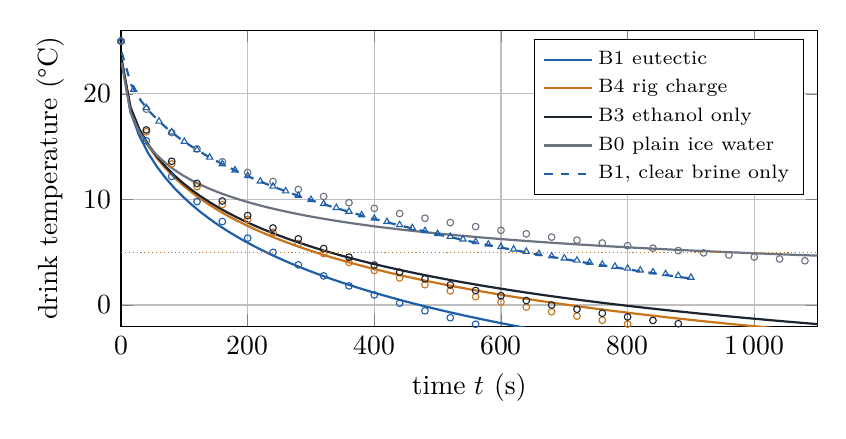
\begin{tikzpicture}
\begin{axis}[width=0.86\linewidth, height=0.44\linewidth, xlabel={time $t$ (s)}, ylabel={drink temperature (\textdegree C)},
  xmin=0, xmax=1100, ymin=-2, ymax=26, grid=major, legend cell align=left, legend style={font=\scriptsize, at={(0.98,0.97)}, anchor=north east}]
\addplot[cBlue, thick] coordinates {(1,23.12) (14.91,18.29) (28.82,16.03) (42.73,14.4) (56.65,13.1) (70.56,12.01) (84.47,11.06) (98.38,10.22) (112.3,9.461) (126.2,8.773) (140.1,8.142) (154,7.559) (167.9,7.016) (181.8,6.509) (195.8,6.032) (209.7,5.583) (223.6,5.159) (237.5,4.756) (251.4,4.374) (265.3,4.009) (279.2,3.66) (293.1,3.327) (307.1,3.008) (321,2.701) (334.9,2.406) (348.8,2.122) (362.7,1.848) (376.6,1.584) (390.5,1.329) (404.4,1.082) (418.3,0.8426) (432.3,0.611) (446.2,0.3864) (460.1,0.1685) (474,-0.04323) (487.9,-0.249) (501.8,-0.4491) (515.7,-0.6438) (529.6,-0.8335) (543.5,-1.018) (557.5,-1.198) (571.4,-1.374) (585.3,-1.546) (599.2,-1.713) (613.1,-1.877) (627,-2.036) (640.9,-2.193) (654.8,-2.345) (668.7,-2.495) (682.7,-2.641) (696.6,-2.784) (710.5,-2.925) (724.4,-3.062) (738.3,-3.197) (752.2,-3.329) (766.1,-3.459) (780,-3.586) (793.9,-3.71) (807.9,-3.833) (821.8,-3.953) (835.7,-4.071) (849.6,-4.187) (863.5,-4.301) (877.4,-4.413) (891.3,-4.523) (905.2,-4.631) (919.2,-4.737) (933.1,-4.842) (947,-4.945) (960.9,-5.046) (974.8,-5.146) (988.7,-5.244) (1003,-5.341) (1017,-5.436) (1030,-5.53) (1044,-5.622) (1058,-5.713) (1072,-5.803) (1086,-5.891) (1100,-5.978)};
\addlegendentry{B1 eutectic}
\addplot[cBlue, only marks, mark=o, mark size=1.2pt, forget plot] coordinates {(0,25) (40,15.55) (80,12.18) (120,9.79) (160,7.903) (200,6.332) (240,4.983) (280,3.801) (320,2.75) (360,1.805) (400,0.9479) (440,0.1657) (480,-0.5519) (520,-1.213) (560,-1.826) (600,-2.395) (640,-2.924) (680,-3.417) (720,-3.878) (760,-4.31) (800,-4.714) (840,-5.092) (880,-5.447) (920,-5.78) (960,-6.092) (1000,-6.384) (1040,-6.658) (1080,-6.914)};
\addplot[cAmber, thick] coordinates {(1,23.21) (14.91,18.67) (28.82,16.58) (42.73,15.09) (56.65,13.91) (70.56,12.92) (84.47,12.06) (98.38,11.31) (112.3,10.64) (126.2,10.02) (140.1,9.465) (154,8.95) (167.9,8.472) (181.8,8.027) (195.8,7.61) (209.7,7.217) (223.6,6.847) (237.5,6.497) (251.4,6.165) (265.3,5.849) (279.2,5.548) (293.1,5.261) (307.1,4.985) (321,4.722) (334.9,4.468) (348.8,4.225) (362.7,3.991) (376.6,3.765) (390.5,3.547) (404.4,3.337) (418.3,3.133) (432.3,2.937) (446.2,2.746) (460.1,2.561) (474,2.382) (487.9,2.208) (501.8,2.039) (515.7,1.875) (529.6,1.715) (543.5,1.559) (557.5,1.408) (571.4,1.26) (585.3,1.116) (599.2,0.9759) (613.1,0.8389) (627,0.7051) (640.9,0.5745) (654.8,0.4468) (668.7,0.322) (682.7,0.2) (696.6,0.08056) (710.5,-0.03629) (724.4,-0.1507) (738.3,-0.2627) (752.2,-0.3725) (766.1,-0.4801) (780,-0.5855) (793.9,-0.6889) (807.9,-0.7903) (821.8,-0.8898) (835.7,-0.9874) (849.6,-1.083) (863.5,-1.177) (877.4,-1.27) (891.3,-1.361) (905.2,-1.45) (919.2,-1.538) (933.1,-1.624) (947,-1.708) (960.9,-1.792) (974.8,-1.874) (988.7,-1.954) (1003,-2.034) (1017,-2.112) (1030,-2.189) (1044,-2.265) (1058,-2.339) (1072,-2.413) (1086,-2.485) (1100,-2.556)};
\addlegendentry{B4 rig charge}
\addplot[cAmber, only marks, mark=o, mark size=1.2pt, forget plot] coordinates {(0,25) (40,16.41) (80,13.36) (120,11.21) (160,9.505) (200,8.092) (240,6.88) (280,5.819) (320,4.877) (360,4.031) (400,3.263) (440,2.564) (480,1.922) (520,1.33) (560,0.7817) (600,0.2729) (640,-0.201) (680,-0.6435) (720,-1.057) (760,-1.444) (800,-1.807) (840,-2.149) (880,-2.469) (920,-2.771) (960,-3.055) (1000,-3.323) (1040,-3.575) (1080,-3.812)};
\addplot[cInk, thick] coordinates {(1,23.22) (14.91,18.73) (28.82,16.68) (42.73,15.22) (56.65,14.06) (70.56,13.09) (84.47,12.26) (98.38,11.52) (112.3,10.86) (126.2,10.27) (140.1,9.727) (154,9.227) (167.9,8.764) (181.8,8.333) (195.8,7.929) (209.7,7.549) (223.6,7.192) (237.5,6.854) (251.4,6.533) (265.3,6.228) (279.2,5.938) (293.1,5.66) (307.1,5.395) (321,5.141) (334.9,4.898) (348.8,4.664) (362.7,4.438) (376.6,4.221) (390.5,4.012) (404.4,3.81) (418.3,3.615) (432.3,3.426) (446.2,3.243) (460.1,3.066) (474,2.894) (487.9,2.728) (501.8,2.566) (515.7,2.408) (529.6,2.255) (543.5,2.107) (557.5,1.962) (571.4,1.82) (585.3,1.683) (599.2,1.549) (613.1,1.418) (627,1.29) (640.9,1.165) (654.8,1.043) (668.7,0.9242) (682.7,0.8077) (696.6,0.6938) (710.5,0.5823) (724.4,0.4732) (738.3,0.3663) (752.2,0.2617) (766.1,0.1592) (780,0.05872) (793.9,-0.03978) (807.9,-0.1364) (821.8,-0.2311) (835.7,-0.3241) (849.6,-0.4153) (863.5,-0.5049) (877.4,-0.5929) (891.3,-0.6793) (905.2,-0.7641) (919.2,-0.8475) (933.1,-0.9295) (947,-1.01) (960.9,-1.089) (974.8,-1.167) (988.7,-1.244) (1003,-1.319) (1017,-1.394) (1030,-1.467) (1044,-1.538) (1058,-1.609) (1072,-1.679) (1086,-1.748) (1100,-1.815)};
\addlegendentry{B3 ethanol only}
\addplot[cInk, only marks, mark=o, mark size=1.2pt, forget plot] coordinates {(0,25) (40,16.58) (80,13.61) (120,11.51) (160,9.849) (200,8.472) (240,7.293) (280,6.261) (320,5.346) (360,4.523) (400,3.779) (440,3.099) (480,2.476) (520,1.902) (560,1.371) (600,0.8779) (640,0.4192) (680,-0.008874) (720,-0.4092) (760,-0.7843) (800,-1.136) (840,-1.466) (880,-1.776) (920,-2.068) (960,-2.343) (1000,-2.602) (1040,-2.846) (1080,-3.075)};
\addplot[cGrey, thick] coordinates {(1,22.93) (14.91,18.27) (28.82,16.38) (42.73,15.13) (56.65,14.18) (70.56,13.42) (84.47,12.79) (98.38,12.25) (112.3,11.78) (126.2,11.37) (140.1,11) (154,10.66) (167.9,10.36) (181.8,10.08) (195.8,9.822) (209.7,9.584) (223.6,9.363) (237.5,9.157) (251.4,8.964) (265.3,8.783) (279.2,8.612) (293.1,8.451) (307.1,8.299) (321,8.154) (334.9,8.016) (348.8,7.885) (362.7,7.76) (376.6,7.641) (390.5,7.527) (404.4,7.417) (418.3,7.312) (432.3,7.212) (446.2,7.115) (460.1,7.021) (474,6.931) (487.9,6.845) (501.8,6.761) (515.7,6.68) (529.6,6.602) (543.5,6.526) (557.5,6.453) (571.4,6.382) (585.3,6.313) (599.2,6.247) (613.1,6.182) (627,6.119) (640.9,6.057) (654.8,5.998) (668.7,5.94) (682.7,5.883) (696.6,5.828) (710.5,5.775) (724.4,5.723) (738.3,5.672) (752.2,5.622) (766.1,5.573) (780,5.526) (793.9,5.48) (807.9,5.434) (821.8,5.39) (835.7,5.347) (849.6,5.305) (863.5,5.263) (877.4,5.223) (891.3,5.183) (905.2,5.144) (919.2,5.106) (933.1,5.068) (947,5.032) (960.9,4.996) (974.8,4.961) (988.7,4.926) (1003,4.892) (1017,4.859) (1030,4.826) (1044,4.794) (1058,4.762) (1072,4.731) (1086,4.701) (1100,4.671)};
\addlegendentry{B0 plain ice water}
\addplot[cGrey, only marks, mark=o, mark size=1.2pt, forget plot] coordinates {(0,25) (40,18.55) (80,16.33) (120,14.78) (160,13.56) (200,12.55) (240,11.69) (280,10.94) (320,10.28) (360,9.686) (400,9.15) (440,8.661) (480,8.214) (520,7.802) (560,7.42) (600,7.067) (640,6.737) (680,6.429) (720,6.141) (760,5.87) (800,5.616) (840,5.376) (880,5.15) (920,4.936) (960,4.734) (1000,4.542) (1040,4.359) (1080,4.187)};
\addplot[cBlue, thick, dashed] coordinates {(1,23.93) (16.24,20.85) (31.47,19.34) (46.71,18.21) (61.95,17.29) (77.19,16.49) (92.42,15.79) (107.7,15.16) (122.9,14.58) (138.1,14.04) (153.4,13.55) (168.6,13.08) (183.8,12.65) (199.1,12.23) (214.3,11.84) (229.6,11.46) (244.8,11.11) (260,10.77) (275.3,10.44) (290.5,10.12) (305.7,9.82) (321,9.528) (336.2,9.245) (351.5,8.972) (366.7,8.708) (381.9,8.451) (397.2,8.202) (412.4,7.96) (427.6,7.725) (442.9,7.496) (458.1,7.274) (473.4,7.056) (488.6,6.845) (503.8,6.638) (519.1,6.436) (534.3,6.239) (549.5,6.046) (564.8,5.858) (580,5.673) (595.3,5.492) (610.5,5.315) (625.7,5.142) (641,4.972) (656.2,4.805) (671.4,4.642) (686.7,4.481) (701.9,4.323) (717.2,4.169) (732.4,4.017) (747.6,3.867) (762.9,3.72) (778.1,3.576) (793.3,3.434) (808.6,3.294) (823.8,3.157) (839.1,3.021) (854.3,2.888) (869.5,2.757) (884.8,2.627) (900,2.5)};
\addlegendentry{B1, clear brine only}
\addplot[cBlue, only marks, mark=triangle, mark size=1.3pt, forget plot] coordinates {(0,25) (20,20.42) (40,18.68) (60,17.4) (80,16.37) (100,15.48) (120,14.7) (140,13.99) (160,13.36) (180,12.77) (200,12.23) (220,11.72) (240,11.24) (260,10.79) (280,10.37) (300,9.965) (320,9.58) (340,9.213) (360,8.862) (380,8.525) (400,8.201) (420,7.889) (440,7.588) (460,7.298) (480,7.018) (500,6.746) (520,6.484) (540,6.229) (560,5.981) (580,5.741) (600,5.507) (620,5.279) (640,5.058) (660,4.842) (680,4.631) (700,4.426) (720,4.226) (740,4.03) (760,3.838) (780,3.651) (800,3.468) (820,3.289) (840,3.114) (860,2.942) (880,2.773) (900,2.608)};
\addplot[cAmber, densely dotted, forget plot] coordinates {(0,5) (1100,5)};
\end{axis}
\end{tikzpicture}
\caption{Drink temperature for a well-mixed Can 2 (side wall only, as in the check), from Eq.~\eqref{eq:erfcx} (lines) and from the full numerical solution (symbols).}
\label{fig:curves}
\end{figure}

\subsection{Results for your rig}\label{sec:res}
Full can (side wall, bottom and fin), Can 2 with 330\,mL, base \val{zzero}\,cm off the floor, $\varphi_p=\val{phip}$, cooling 25\,$\to$\,5\,\textdegree C:
\begin{center}\footnotesize
\begin{tabular}{@{}l l r r r r r r@{}}
\toprule
recipe & ice held & $T_b$ (\textdegree C) & $E$ slush & $t_5$ (s) & rate at 15\,\textdegree C & rate at 5\,\textdegree C & mean rate \\
 & & & (W\,s$^{1/2}$m$^{-2}$K$^{-1}$) & & (K/min) & (K/min) & (K/min) \\
\midrule
B0 plain ice & floor & $\val{B0Tbone}$ & \val{B0FoEs} & \val{B0Fot} & \val{B0Forfifteen} & \val{B0Forfive} & \val{B0Formean} \\
B1 eutectic & floats & $\val{B1Tbone}$ & \val{B1FlEs} & \val{B1Flt} & \val{B1Flrfifteen} & \val{B1Flrfive} & \val{B1Flrmean} \\
 & board & & \val{B1BdEs} & \val{B1Bdt} & \val{B1Bdrfifteen} & \val{B1Bdrfive} & \val{B1Bdrmean} \\
 & floor & & \val{B1FoEs} & \val{B1Fot} & \val{B1Forfifteen} & \val{B1Forfive} & \val{B1Formean} \\
B2 salt + ethanol & board & $\val{B2Tbone}$ & \val{B2BdEs} & \val{B2Bdt} & \val{B2Bdrfifteen} & \val{B2Bdrfive} & \val{B2Bdrmean} \\
 & floor & & \val{B2FoEs} & \val{B2Fot} & \val{B2Forfifteen} & \val{B2Forfive} & \val{B2Formean} \\
B3 ethanol only & board & $\val{B3Tbone}$ & \val{B3BdEs} & \val{B3Bdt} & \val{B3Bdrfifteen} & \val{B3Bdrfive} & \val{B3Bdrmean} \\
 & floor & & \val{B3FoEs} & \val{B3Fot} & \val{B3Forfifteen} & \val{B3Forfive} & \val{B3Formean} \\
B4 original charge & board & $\val{B4Tbone}$ & \val{B4BdEs} & \val{B4Bdt} & \val{B4Bdrfifteen} & \val{B4Bdrfive} & \val{B4Bdrmean} \\
 & floor & & \val{B4FoEs} & \val{B4Fot} & \val{B4Forfifteen} & \val{B4Forfive} & \val{B4Formean} \\
\bottomrule
\end{tabular}
\end{center}
What the table says:
\begin{itemize}
\item \textbf{Salt pays}, even with no convection. Going from plain ice water to the eutectic cuts the time by \val{SpeedSalt}\,\texttimes{} with the ice at the floor.
\item \textbf{Ice placement pays almost as much.} Slush around the whole drink column beats a floating pack by \val{RatioFloorFl}\,\texttimes. Clear brine has no latent store, so its effusivity is only $\val{B1BdEbr}$.
\item \textbf{Ethanol does not pay here.} B2 is only slightly faster than B1 despite being 3\,K colder. B3 (ethanol only) is much slower because it is warmer and has melted more of the ice.
\item \textbf{B4 is slow for a geometric reason as much as a thermal one:} with a lid board almost all of its drink column sits in clear brine.
\end{itemize}

\textbf{A check against published data.} SINTEF timed a 0.33\,L can from 21 to 5\,\textdegree C: about 600\,s in ice water and 150\,s in a $-16$\,\textdegree C salt bath. The same calculation (21\,\textdegree C start, Can 2, ice at the floor, $m_s=\val{SiMs}$\,kg for $-16$\,\textdegree C) gives \val{SiIce}\,s and \val{SiSix}\,s (\val{SiSixBd}\,s with a lid board). With no convection inside the drink either, the full numerical solution gives \val{SiCondIce}\,s and \val{SiCondSix}\,s. Both measurements sit near the well-mixed limit and far from the no-convection-inside limit: a real drink mixes itself well by natural convection. The ice-water measurement is about a third slower than the well-mixed prediction, which is what you would expect if water rather than packed slush surrounded part of the can.

\subsection{No convection inside the drink either}\label{sec:conduct}
Taken literally, ``disregard convection'' also stops the drink from mixing, so heat has to diffuse through it too. This is the \textbf{true minimum cooling rate}: any convection, inside or outside, can only speed things up.

\textbf{The contact temperature.} Two materials of effusivity $E_d=\sqrt{k_d\rho_dc_d}$ (drink, \val{CdBoneEd}) and $E$ (slush) brought into contact at once jump to a common surface temperature. To leading order it stays there:
\begin{equation}
\boxed{\;T_c=\frac{E_d\,T_0+E\,T_b}{E_d+E}\;}
\label{eq:Tc}
\end{equation}
For B1, $T_c=\val{CdBoneTc}$\,\textdegree C; the full numerical solution's wall temperature after 300\,s is $\val{CdBoneTw}$\,\textdegree C.
\begin{warn}[The drink at the wall must supercool or freeze]
$T_c$ is far below the drink's freezing point ($-0.77$\,\textdegree C). In a no-convection world the layer of drink against the wall either supercools, which canned drinks often do, or freezes onto the wall while the centre is still near 25\,\textdegree C. The numbers below assume it supercools; freezing would add a second moving front.
\end{warn}

\textbf{Closed form for the mean drink temperature.} Inside a solid cylinder the response, to the same order, is $E_d\sqrt s-k_d/2r_i$. The curvature now \emph{reduces} the flux, because the inside runs out of heat. Matching it to the outside response $E\sqrt s+k/2R$ at the wall and inverting the transform (Appendix~\ref{sec:lap}) gives
\begin{equation}
\boxed{\;\frac{\bar\Theta(t)}{\Theta_0}=1-\frac{A}{C\,D}\big[E_dE\,f_2+\beta\,f_3-\gamma\,f_4\big]\;}
\label{eq:conduct}
\end{equation}
\[
\begin{aligned}
&D=E_d+E,\qquad g_d=\frac{k_d}{2r_i},\qquad g_s=\frac{k}{2R},\qquad c=\frac{g_s-g_d}{D},\qquad \beta=E_dg_s-Eg_d,\qquad \gamma=g_dg_s,\\
&f_1=\erfcx(c\sqrt t),\qquad f_2=\frac{1-f_1}{c},\qquad f_3=\frac{1}{c}\Big(2\sqrt{\frac t\pi}-f_2\Big),\qquad f_4=\frac{1}{c}\,(t-f_3).
\end{aligned}
\]
It needs a single $\erfcx$ and holds while the drink's Fourier number $\alpha_dt/r_i^2\lesssim0.15$. For a linear outside medium it agrees with the full solution to 4\,\%. In slush it is \val{CdBoneerr}\,\% (B1) and \val{CdBfourerr}\,\% (B4) against the full solution, because the wall temperature drifts down through the partly melted range. Use the full-solution numbers as the bound:
\begin{center}\footnotesize
\begin{tabular}{@{}l r r r r r@{}}
\toprule
 & $T_c$ (\textdegree C) & $t_5$ mean, full solution & $t_5$ mean, Eq.~\eqref{eq:conduct} & $t_5$ centre, full solution & rate at 5\,\textdegree C (full) \\
\midrule
B1 & $\val{CdBoneTc}$ & \val{CdBonetp}\,s & \val{CdBonetcf}\,s & \val{CdBonetcore}\,s & \val{CdBonerp}\,K/min \\
B4 & $\val{CdBfourTc}$ & \val{CdBfourtp}\,s & \val{CdBfourtcf}\,s & \val{CdBfourtcore}\,s & \val{CdBfourrp}\,K/min \\
\bottomrule
\end{tabular}
\end{center}
So for B1 the drink's mean temperature takes about \val{CdBonetp}\,s, and its centre \val{CdBonetcore}\,s, compared with \val{B1Fot}--\val{B1Flt}\,s for a well-mixed drink. These are side-wall-only numbers, which is conservative, as a bound should be.

\begin{figure}[H]
\centering

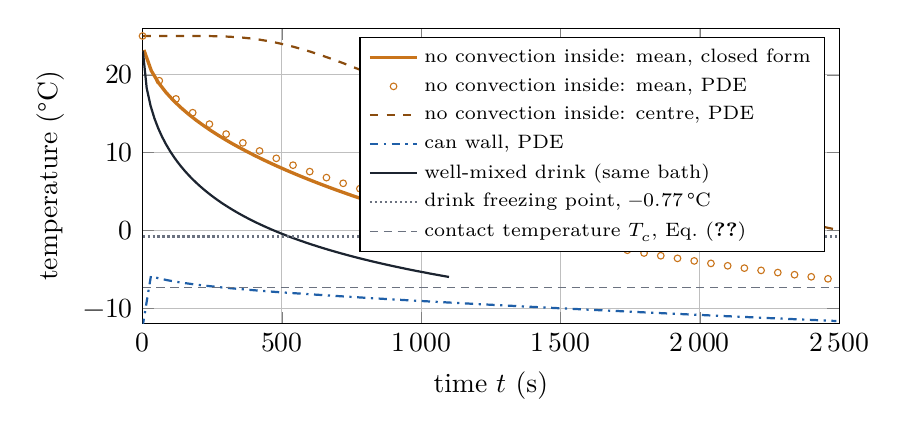
\begin{tikzpicture}
\begin{axis}[width=0.86\linewidth, height=0.44\linewidth, xlabel={time $t$ (s)}, ylabel={temperature (\textdegree C)},
  xmin=0, xmax=2500, ymin=-12, ymax=26, grid=major, legend cell align=left, legend style={font=\scriptsize, at={(0.98,0.97)}, anchor=north east}]
\addplot[cAmber, very thick] coordinates {(5,23.2) (31.43,20.53) (57.86,18.96) (84.29,17.74) (110.7,16.71) (137.1,15.81) (163.6,14.99) (190,14.24) (216.4,13.55) (242.9,12.9) (269.3,12.29) (295.7,11.71) (322.1,11.16) (348.6,10.64) (375,10.14) (401.4,9.654) (427.9,9.188) (454.3,8.739) (480.7,8.305) (507.1,7.884) (533.6,7.476) (560,7.08) (586.4,6.695) (612.9,6.319) (639.3,5.954) (665.7,5.597) (692.1,5.249) (718.6,4.908) (745,4.575) (771.4,4.249) (797.9,3.93) (824.3,3.618) (850.7,3.312) (877.1,3.011) (903.6,2.716) (930,2.426) (956.4,2.142) (982.9,1.863) (1009,1.588) (1036,1.318) (1062,1.052) (1089,0.7903) (1115,0.5329) (1141,0.2794) (1168,0.02964) (1194,-0.2164) (1221,-0.4589) (1247,-0.6979) (1274,-0.9335) (1300,-1.166)};
\addlegendentry{no convection inside: mean, closed form}
\addplot[cAmber, only marks, mark=o, mark size=1.2pt] coordinates {(0,25) (60,19.25) (120,16.91) (180,15.14) (240,13.67) (300,12.39) (360,11.26) (420,10.22) (480,9.271) (540,8.39) (600,7.567) (660,6.793) (720,6.062) (780,5.369) (840,4.709) (900,4.08) (960,3.479) (1020,2.904) (1080,2.351) (1140,1.821) (1200,1.311) (1260,0.8201) (1320,0.3469) (1380,-0.1094) (1440,-0.5499) (1500,-0.9753) (1560,-1.386) (1620,-1.784) (1680,-2.169) (1740,-2.541) (1800,-2.901) (1860,-3.251) (1920,-3.589) (1980,-3.917) (2040,-4.235) (2100,-4.544) (2160,-4.844) (2220,-5.135) (2280,-5.417) (2340,-5.692) (2400,-5.958) (2460,-6.218)};
\addlegendentry{no convection inside: mean, PDE}
\addplot[cAmberDark, thick, dashed] coordinates {(0,25) (30,25) (60,25) (90,25) (120,25) (150,25) (180,25) (210,25) (240,24.99) (270,24.97) (300,24.93) (330,24.87) (360,24.79) (390,24.68) (420,24.53) (450,24.35) (480,24.14) (510,23.9) (540,23.63) (570,23.33) (600,23.01) (630,22.66) (660,22.29) (690,21.91) (720,21.51) (750,21.09) (780,20.67) (810,20.23) (840,19.79) (870,19.34) (900,18.89) (930,18.43) (960,17.97) (990,17.51) (1020,17.05) (1050,16.59) (1080,16.13) (1110,15.68) (1140,15.22) (1170,14.77) (1200,14.33) (1230,13.89) (1260,13.45) (1290,13.02) (1320,12.59) (1350,12.17) (1380,11.75) (1410,11.34) (1440,10.93) (1470,10.53) (1500,10.14) (1530,9.748) (1560,9.365) (1590,8.988) (1620,8.616) (1650,8.25) (1680,7.89) (1710,7.536) (1740,7.187) (1770,6.844) (1800,6.506) (1830,6.174) (1860,5.847) (1890,5.526) (1920,5.21) (1950,4.899) (1980,4.593) (2010,4.293) (2040,3.997) (2070,3.706) (2100,3.42) (2130,3.139) (2160,2.863) (2190,2.591) (2220,2.324) (2250,2.061) (2280,1.802) (2310,1.548) (2340,1.298) (2370,1.052) (2400,0.8098) (2430,0.5719) (2460,0.3378) (2490,0.1076)};
\addlegendentry{no convection inside: centre, PDE}
\addplot[cBlue, thick, dashdotted] coordinates {(0,-12.4) (30,-5.867) (60,-6.177) (90,-6.404) (120,-6.595) (150,-6.759) (180,-6.905) (210,-7.037) (240,-7.159) (270,-7.273) (300,-7.374) (330,-7.471) (360,-7.565) (390,-7.657) (420,-7.745) (450,-7.83) (480,-7.913) (510,-7.984) (540,-8.056) (570,-8.13) (600,-8.202) (630,-8.273) (660,-8.343) (690,-8.412) (720,-8.48) (750,-8.547) (780,-8.613) (810,-8.678) (840,-8.742) (870,-8.806) (900,-8.868) (930,-8.93) (960,-8.991) (990,-9.052) (1020,-9.111) (1050,-9.171) (1080,-9.229) (1110,-9.287) (1140,-9.345) (1170,-9.402) (1200,-9.459) (1230,-9.516) (1260,-9.572) (1290,-9.627) (1320,-9.682) (1350,-9.737) (1380,-9.792) (1410,-9.846) (1440,-9.9) (1470,-9.954) (1500,-10.01) (1530,-10.06) (1560,-10.11) (1590,-10.17) (1620,-10.22) (1650,-10.27) (1680,-10.32) (1710,-10.37) (1740,-10.43) (1770,-10.48) (1800,-10.53) (1830,-10.58) (1860,-10.63) (1890,-10.68) (1920,-10.73) (1950,-10.78) (1980,-10.83) (2010,-10.88) (2040,-10.93) (2070,-10.98) (2100,-11.03) (2130,-11.07) (2160,-11.12) (2190,-11.17) (2220,-11.22) (2250,-11.27) (2280,-11.31) (2310,-11.36) (2340,-11.41) (2370,-11.46) (2400,-11.5) (2430,-11.55) (2460,-11.6) (2490,-11.64)};
\addlegendentry{can wall, PDE}
\addplot[cInk, thick] coordinates {(1,23.12) (14.91,18.29) (28.82,16.03) (42.73,14.4) (56.65,13.1) (70.56,12.01) (84.47,11.06) (98.38,10.22) (112.3,9.461) (126.2,8.773) (140.1,8.142) (154,7.559) (167.9,7.016) (181.8,6.509) (195.8,6.032) (209.7,5.583) (223.6,5.159) (237.5,4.756) (251.4,4.374) (265.3,4.009) (279.2,3.66) (293.1,3.327) (307.1,3.008) (321,2.701) (334.9,2.406) (348.8,2.122) (362.7,1.848) (376.6,1.584) (390.5,1.329) (404.4,1.082) (418.3,0.8426) (432.3,0.611) (446.2,0.3864) (460.1,0.1685) (474,-0.04323) (487.9,-0.249) (501.8,-0.4491) (515.7,-0.6438) (529.6,-0.8335) (543.5,-1.018) (557.5,-1.198) (571.4,-1.374) (585.3,-1.546) (599.2,-1.713) (613.1,-1.877) (627,-2.036) (640.9,-2.193) (654.8,-2.345) (668.7,-2.495) (682.7,-2.641) (696.6,-2.784) (710.5,-2.925) (724.4,-3.062) (738.3,-3.197) (752.2,-3.329) (766.1,-3.459) (780,-3.586) (793.9,-3.71) (807.9,-3.833) (821.8,-3.953) (835.7,-4.071) (849.6,-4.187) (863.5,-4.301) (877.4,-4.413) (891.3,-4.523) (905.2,-4.631) (919.2,-4.737) (933.1,-4.842) (947,-4.945) (960.9,-5.046) (974.8,-5.146) (988.7,-5.244) (1003,-5.341) (1017,-5.436) (1030,-5.53) (1044,-5.622) (1058,-5.713) (1072,-5.803) (1086,-5.891) (1100,-5.978)};
\addlegendentry{well-mixed drink (same bath)}
\addplot[cGrey, densely dotted, thick] coordinates {(0,-0.77) (2500,-0.77)};
\addlegendentry{drink freezing point, $-0.77$\,\textdegree C}
\addplot[cGrey, densely dashed] coordinates {(0,-7.377) (2500,-7.377)};
\addlegendentry{contact temperature $T_c$, Eq.~\eqref{eq:Tc}}
\end{axis}
\end{tikzpicture}
\caption{B1, Can 2, side wall only: with no convection inside the drink, the wall drops at once to about $T_c$ and stays below the drink's freezing point. The mean temperature falls like $\sqrt t$ and the centre lags far behind. The well-mixed drink in the same bath is shown for comparison.}
\label{fig:conduct}
\end{figure}

% =====================================================================================================
\section{The whole chain, design and what to measure}\label{sec:chain}

\subsection{From your four masses to the drink temperature}\label{sec:algo}
\begin{result}[Evaluation order: each line uses only quantities from the lines above and the measured constants]
\small
\begin{enumerate}[leftmargin=1.6em, label=\textbf{\arabic*.}]
\item Active solute $n_s',n_e'$ \hfill Eq.~\eqref{eq:active}
\item Heat capacities $C_r$, $C_\theta$ \hfill Eq.~\eqref{eq:Cs}
\item Depression strength $N$ and bound water $W_b$ \hfill Eq.~\eqref{eq:liq}
\item $A,B,Q_0$; bath depression $\theta_U$; then $W$, $x$ \hfill Eqs.~\eqref{eq:quad}, \eqref{eq:thetaU}
\item If saturated: $W_S$ and $\theta_S$. If $x>m_i$: $\theta_I$ \hfill Eqs.~\eqref{eq:WS}--\eqref{eq:thetaI}
\item With ethanol: update $h_E$, $c_{ea}$ at $b_e=n_e'/W$ and repeat 1--5 once \hfill \S\ref{sec:twopass}
\item Brine: $b_s=n_d/W$, $b_e=n_e'/W$, $m_b$, $w_s$, $w_e$, $\rho_b$ \hfill \S\ref{sec:layers}
\item Can: $r_i$, $h_d$, $V_a$, $C$, $M_c$ \hfill Eqs.~\eqref{eq:can}, \eqref{eq:canC}
\item Tank: $V_I$, $V_b$, $h_p$, $V_p$, then the layers for your way of holding the ice \hfill Eqs.~\eqref{eq:vols}, \eqref{eq:float}
\item Contact lengths and areas $A_{sl}$, $A_{br}$, $A_{\rm bot}$ \hfill Eq.~\eqref{eq:areas}
\item Slush at the can: $W_0$, $m_{I0}$, $N_v$, $W_{b,v}$; then $\theta_L$, $\eta_c$, $C_v$, $\Delta H$, $c_m$, $k_m$ \hfill Eqs.~\eqref{eq:slush}--\eqref{eq:dH}
\item Effusivity: $T_{\rm ref}$, then $\lambda$, $E$, $k$; clear brine $E_{br}$ \hfill Eqs.~\eqref{eq:Tref}, \eqref{eq:neumann}--\eqref{eq:keff}
\item Cooling: $a$, $b$, $p_{1,2}$; $T_d(t)$; $t_5$; rate; $\bar T$; $\bar h$; fin $A_{\rm fin}$ \hfill Eqs.~\eqref{eq:ab}--\eqref{eq:hbar}, \eqref{eq:fin}
\item Repeat 12--13 twice (the reference temperature and the fin settle)
\item Strict lower bound, no convection inside: $T_c$ and $\bar\Theta(t)$ \hfill Eqs.~\eqref{eq:Tc}, \eqref{eq:conduct}
\end{enumerate}
The only numerical steps are two scalar roots, $\lambda$ in Eq.~\eqref{eq:neumann} and $t_5$ in Eq.~\eqref{eq:erfcx}; both functions are monotonic. Everything else is explicit.
\end{result}

\subsection{What depends on what}\label{sec:deps}
\begin{center}\footnotesize
\renewcommand{\arraystretch}{1.1}
\begin{tabularx}{\linewidth}{@{}l X l@{}}
\toprule
derived quantity & is a function of & equation \\
\midrule
\der\ $n_s',\;n_e'$ & $m_s,\,m_e;\ \eta_s,\eta_e$ & \eqref{eq:active} \\
\der\ $C_r,\;C_\theta$ & $m_w,m_s,m_e,m_i;\ c$'s, $\eta_e$ & \eqref{eq:Cs} \\
\der\ $N,\;W_b$ & $n_s',n_e';\ K_s,K_e,\omega_s,\omega_e$ & \eqref{eq:liq} \\
\der\ $\theta_b\ (=-T_b)$ & $m_w,m_s,m_e,m_i;\ T_r;\ L_0,\Delta c,\Delta h_s,h_E,K$'s, $\omega$'s, $b_E,\theta_E,\lambda;\ \eta_s,\eta_e$ & \eqref{eq:thetaU}, \eqref{eq:WS}, \eqref{eq:cot}, \eqref{eq:thetaI} \\
\der\ $W,\;x,\;n_d$ & as $\theta_b$ & same \\
\der\ $\rho_b,\;m_b,\;V_b,\;V_I$ & $W,n_d,n_e',x;\ \rho_0,\beta_s,\beta_e,\rho_i$ & \eqref{eq:vols} \\
\der\ $h_d,\;V_a,\;C,\;M_c$ & $V_d,R,H,t_w,m_{\rm Al};\ \rho_d,c_d,c_{\rm Al}$ & \eqref{eq:can}, \eqref{eq:canC} \\
\der\ layers $h_{cb},h_b,h_p$ & $V_b,V_I,\rho_b;\ A_t,R,\varphi_p$; how the ice is held & \eqref{eq:float} \\
\der\ $L_{sl},L_{br},A$'s & layers; $z_0,h_d,H,R$ & \eqref{eq:areas} \\
\der\ $\theta_L,\;\eta_c$ & $\theta_b$, brine composition, $\rho_b;\ \varphi_p,\rho_i$ & \eqref{eq:etac} \\
\der\ $\Delta H,\;C_v,\;c_m,\;k_m$ & $\theta_b,\theta_L$, slush composition; $L_0,\Delta c$, $c$'s, $k_i,k_b$ & \eqref{eq:H}, \eqref{eq:dH} \\
\der\ $\lambda,\;E,\;k$ & $T_{\rm ref},T_b,T_L;\ k_l,C_v,k_m,c_m$ & \eqref{eq:neumann}--\eqref{eq:keff} \\
\der\ $a,\;b,\;p_{1,2}$ & $A$'s, $E,k,E_{br},k_b,C,R$ & \eqref{eq:ab}, \eqref{eq:abzones} \\
\der\ $T_d(t),\;t_5$, rate & $a,b,T_b,T_0;\ T_1$ & \eqref{eq:erfcx}, \eqref{eq:rate} \\
\der\ $T_c$, $\bar\Theta(t)$ (no convection inside) & $E_d,E,k,k_d,r_i,R,A/C,T_0,T_b$ & \eqref{eq:Tc}, \eqref{eq:conduct} \\
\bottomrule
\end{tabularx}
\end{center}

\subsection{Design: what each mass does to the time}\label{sec:design}
\begin{figure}[H]
\centering

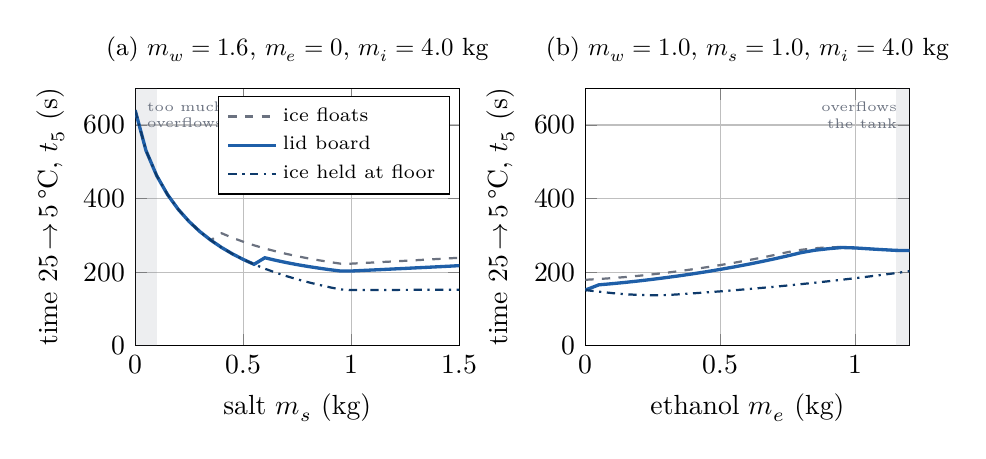
\begin{tikzpicture}
\begin{groupplot}[group style={group size=2 by 1, horizontal sep=16mm}, width=0.47\linewidth, height=0.40\linewidth,
  ylabel={time 25\,$\to$\,5\,\textdegree C, $t_5$ (s)}, grid=major, ymin=0, legend cell align=left, legend style={font=\scriptsize, at={(0.97,0.97)}, anchor=north east}]
\nextgroupplot[xlabel={salt $m_s$ (kg)}, xmin=0, xmax=1.5, ymax=700, title={\small (a) $m_w=1.6$, $m_e=0$, $m_i=4.0$ kg}]
\fill[cGrey, opacity=0.12] (axis cs:0,0) rectangle (axis cs:0.100,700); \node[font=\tiny, anchor=north west, cGrey, align=left] at (axis cs:0.01,690) {too much ice:\\overflows the tank};
\addplot[cGrey, thick, dashed] coordinates {(0,640.4) (0.05,530.8) (0.1,461.9) (0.15,410.6) (0.2,370.2) (0.25,337.3) (0.3,309.9) (0.35,286.8) (0.4,305.7) (0.45,293.4) (0.5,282.6) (0.55,272.9) (0.6,264.3) (0.65,256.6) (0.7,249.5) (0.75,243.2) (0.8,237.4) (0.85,232.2) (0.9,227.4) (0.95,223) (1,223) (1.05,224.6) (1.1,226.1) (1.15,227.7) (1.2,229.2) (1.25,230.8) (1.3,232.4) (1.35,234.1) (1.4,235.7) (1.45,237.4) (1.5,239)};
\addlegendentry{ice floats}
\addplot[cBlue, very thick] coordinates {(0,640.4) (0.05,530.8) (0.1,461.9) (0.15,410.6) (0.2,370.2) (0.25,337.3) (0.3,309.9) (0.35,286.8) (0.4,266.9) (0.45,249.6) (0.5,234.5) (0.55,221.2) (0.6,239) (0.65,232.1) (0.7,225.9) (0.75,220.3) (0.8,215.3) (0.85,210.8) (0.9,206.6) (0.95,202.9) (1,203) (1.05,204.4) (1.1,205.8) (1.15,207.2) (1.2,208.7) (1.25,210.1) (1.3,211.6) (1.35,213) (1.4,214.5) (1.45,216) (1.5,217.6)};
\addlegendentry{lid board}
\addplot[cDeep, thick, dashdotted] coordinates {(0,640.4) (0.05,530.8) (0.1,461.9) (0.15,410.6) (0.2,370.2) (0.25,337.3) (0.3,309.9) (0.35,286.8) (0.4,266.9) (0.45,249.6) (0.5,234.5) (0.55,221.2) (0.6,209.3) (0.65,198.7) (0.7,189.1) (0.75,180.4) (0.8,172.6) (0.85,165.4) (0.9,158.8) (0.95,152.7) (1,151.3) (1.05,151.4) (1.1,151.5) (1.15,151.5) (1.2,151.6) (1.25,151.7) (1.3,151.8) (1.35,151.8) (1.4,151.9) (1.45,152) (1.5,152.1)};
\addlegendentry{ice held at floor}
\nextgroupplot[xlabel={ethanol $m_e$ (kg)}, xmin=0, xmax=1.2, ymax=700, title={\small (b) $m_w=1.0$, $m_s=1.0$, $m_i=4.0$ kg}]
\fill[cGrey, opacity=0.12] (axis cs:1.150,0) rectangle (axis cs:1.2,700); \node[font=\tiny, anchor=north east, cGrey, align=right] at (axis cs:1.19,690) {overflows\\the tank};
\addplot[cGrey, thick, dashed] coordinates {(0,179.1) (0.05,181.2) (0.1,183.7) (0.15,186.7) (0.2,190.2) (0.25,194) (0.3,198.3) (0.35,202.9) (0.4,208) (0.45,213.4) (0.5,219.2) (0.55,225.4) (0.6,232) (0.65,239) (0.7,246.5) (0.75,254.5) (0.8,260.8) (0.85,264.8) (0.9,267.7) (0.95,268.2) (1,265.7) (1.05,263.3) (1.1,261.1) (1.15,259.1) (1.2,258.5)};
\addplot[cBlue, very thick] coordinates {(0,151.2) (0.05,165.4) (0.1,168.6) (0.15,172.2) (0.2,176.2) (0.25,180.5) (0.3,185.2) (0.35,190.2) (0.4,195.6) (0.45,201.3) (0.5,207.5) (0.55,214) (0.6,220.9) (0.65,228.3) (0.7,236.1) (0.75,244.4) (0.8,253.2) (0.85,259.6) (0.9,263.7) (0.95,266.9) (1,265.7) (1.05,263.3) (1.1,261.1) (1.15,259.1) (1.2,258.5)};
\addplot[cDeep, thick, dashdotted] coordinates {(0,151.2) (0.05,146.8) (0.1,142.9) (0.15,139.7) (0.2,137.9) (0.25,136.9) (0.3,137.5) (0.35,139.8) (0.4,142.3) (0.45,145) (0.5,147.7) (0.55,150.6) (0.6,153.7) (0.65,156.9) (0.7,160.2) (0.75,163.7) (0.8,167.4) (0.85,171.2) (0.9,175.2) (0.95,179.3) (1,183.6) (1.05,188.1) (1.1,192.7) (1.15,197.4) (1.2,202.7)};
\end{groupplot}
\end{tikzpicture}
\caption{Time to cool Can 2 from 25 to 5\,\textdegree C against (a) salt and (b) ethanol, for the three ways of holding the ice. Grey bands: charges that do not fit your 17.5\,cm tank with the can in. The small steps are where clear brine first reaches the can's base, which then sits in brine instead of slush.}
\label{fig:design}
\end{figure}
\begin{itemize}
\item \textbf{Salt (a).} The time falls steeply until the brine saturates, near $m_s^{\ast}$ (Eq.~\eqref{eq:mstar}). Past that point the bath is a thermostat, and extra salt only brings in warm mass that melts a little more ice. With the ice floating or under a board, that ice comes off the pack around the can.
\item \textbf{Ethanol (b).} Each 100\,g lowers $T_b$, but each 100\,g also melts ice through its warmth and its heat of mixing. With no convection the second effect wins sooner than you would guess, because the can ends up in clear brine.
\item \textbf{Ice.} Below saturation, more ice at 0\,\textdegree C makes the bath very slightly \emph{warmer} (\S\ref{sec:sens}). What it really changes is how much slush there is around the can.
\item \textbf{Water.} In regime U, each kilogram of warm water raises $T_b$ by \val{SensBfourmwAbs}\,K. In regime S the temperature stays put, and each kilogram of water instead adds \val{SensBoneWmw}\,kg of liquid water (itself plus the ice it melts).
\end{itemize}

\begin{figure}[H]
\centering

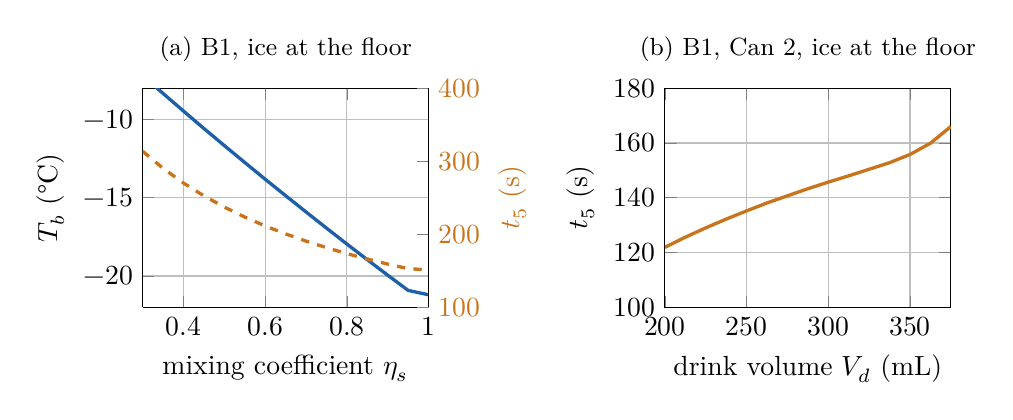
\begin{tikzpicture}
\begin{groupplot}[group style={group size=2 by 1, horizontal sep=30mm}, width=0.43\linewidth, height=0.36\linewidth, grid=major]
\nextgroupplot[xlabel={mixing coefficient $\eta_s$}, ylabel={$T_b$ (\textdegree C)}, xmin=0.3, xmax=1, title={\small (a) B1, ice at the floor},
  axis y line*=left, ymin=-22, ymax=-8]
\addplot[cBlue, very thick] coordinates {(0.3,-7.197) (0.35,-8.339) (0.4,-9.465) (0.45,-10.58) (0.5,-11.67) (0.55,-12.75) (0.6,-13.82) (0.65,-14.87) (0.7,-15.91) (0.75,-16.94) (0.8,-17.96) (0.85,-18.96) (0.9,-19.95) (0.95,-20.92) (1,-21.2)}; \label{pl:etaTb}
\nextgroupplot[xlabel={drink volume $V_d$ (mL)}, ylabel={$t_5$ (s)}, xmin=200, xmax=375, title={\small (b) B1, Can 2, ice at the floor}, ymin=100, ymax=180]
\addplot[cAmber, very thick] coordinates {(200,121.9) (212.5,125.6) (225,129) (237.5,132.2) (250,135.2) (262.5,138.1) (275,140.7) (287.5,143.3) (300,145.7) (312.5,148) (325,150.4) (337.5,152.8) (350,155.8) (362.5,159.9) (375,166)};
\end{groupplot}
\begin{axis}[at={(0,0)}, width=0.43\linewidth, height=0.36\linewidth, xmin=0.3, xmax=1, axis y line*=right, axis x line=none, ylabel={$t_5$ (s)},
  ymin=100, ymax=400, ylabel style={cAmber}, yticklabel style={cAmber}]
\addplot[cAmber, very thick, dashed] coordinates {(0.3,313.6) (0.35,290.2) (0.4,270.1) (0.45,252.6) (0.5,237.2) (0.55,223.5) (0.6,211.4) (0.65,200.5) (0.7,190.6) (0.75,181.7) (0.8,173.5) (0.85,166.1) (0.9,159.2) (0.95,152.9) (1,151.3)};
\end{axis}
\end{tikzpicture}
\caption{(a) B1 with the ice at the floor: bath temperature (blue, left axis) and time to 5\,\textdegree C (amber dashed, right axis) against the salt mixing coefficient $\eta_s$. (b) Time to 5\,\textdegree C against the volume of drink in Can 2: nearly doubling the drink changes the time by about a third.}
\label{fig:etafill}
\end{figure}
With $\eta_s=\val{EtaLow}$ (badly mixed salt) B1 only reaches $\val{EtaTbLow}$\,\textdegree C and needs \val{EtaTLow}\,s. Changing the fill from \val{FillVmin} to \val{FillVmax}\,mL moves $t_5$ only from \val{FillMin} to \val{FillMax}\,s, because the drink's heat capacity and its wetted wall both scale with the fill. What remains comes from the fixed bottom, the aluminium and the shrinking fin.

\subsection{What to measure, and how}\label{sec:measure}
\begin{enumerate}
\item \textbf{$\varphi_p$, the ice packing.} Fill a jug with crushed ice to a mark, top it up with ice water to the same mark, and record the water added: $\varphi_p=1-V_{\rm water}/V_{\rm mark}$. It enters $\eta_c$, the layering and $E$.
\item \textbf{$\eta_s$, the salt mixing.} Let the bath settle (no stirring) and read $T_b$ at least 5\,cm from the can, then apply Eq.~\eqref{eq:etainv}. Do it for each way of adding the salt (all at once, in layers, pre-dissolved).
\item \textbf{The layering.} Mark $h_{cb}$ and $h_b$ on the tank wall and compare with Eq.~\eqref{eq:float}. That tests $\varphi_p$ and $\rho_b$ in one go.
\item \textbf{$T_L$, the diluted brine.} A fine thermocouple bead 2--3\,mm from the can wall should read between $T_L$ and $T_b$ while the can cools (Fig.~\ref{fig:profiles}). If it reads close to $T_b$, convection is carrying the meltwater away and $\eta_c$ is closer to 1 than Eq.~\eqref{eq:etac} says.
\item \textbf{The shape of the cooling curve.} Fit Eq.~\eqref{eq:erfcx} with $E$ as the only free parameter, and also fit an exponential. The ratio $E_{\rm fit}/E_{\rm predicted}$ is a direct measure of how much convection actually helps in your tank: 1 means none.
\end{enumerate}

\subsection{Limits of this model, bluntly}\label{sec:limits}
\begin{itemize}
\item \textbf{Real baths convect.} Meltwater is fresh and light and rises; brine is heavy and sinks. In reality the diluted layer is partly swept away, so the local coefficient lies between $\eta_c$ and 1. Treat this model as the no-flow limit, not a forecast of a stirred tank.
\item \textbf{The well-mixed drink} is an assumption. A real drink sits between the two limits given here, near the well-mixed one according to the SINTEF data.
\item \textbf{The slush as a linear medium} is an approximation: within $\pm$\val{PdeMax}\,\% of the full conduction solution in 16 cases. The reference-temperature rule, Eq.~\eqref{eq:Tref}, is the one empirical step. The bottom and the fin are added by superposition and were not checked against a 2-D solution.
\item \textbf{Bath thermodynamics.} The liquidus is good to \val{ZsrMax}\,K, and the cotectic below $-23.6$\,\textdegree C is extrapolated (B2). $\Delta h_s$, $c_s$ and the ethanol mixing table are placeholders carried over from the earlier model; the $H^E$ table came from a scrambled extraction and needs checking against the paper. Hydrohalite formation and dissolution kinetics are not modelled; $\eta_s$ absorbs them empirically.
\item \textbf{Geometry.} The can is a cylinder (dome and neck ignored) in perfect contact with the slush. The ice pack is uniform, although real packs are looser near walls. The tank height, \val{Ht}\,cm, was inferred, not measured.
\end{itemize}

% =====================================================================================================
\section{Appendix}\label{sec:app}

\subsection{Laplace pairs and the two inversions}\label{sec:lap}
With $\hat f(s)=\int_0^\infty f(t)e^{-st}\,\dd t$, the pairs used are
\[
\mathcal L\{1\}=\frac1s,\quad \mathcal L\{t\}=\frac1{s^2},\quad \mathcal L\Big\{\frac{1}{\sqrt{\pi t}}\Big\}=\frac{1}{\sqrt s},\quad \mathcal L\Big\{2\sqrt{\tfrac t\pi}\Big\}=\frac{1}{s^{3/2}},\quad
\mathcal L\{\erfcx(p\sqrt t)\}=\frac{1}{\sqrt s\,(\sqrt s+p)} .
\]
Writing $1/(\sqrt s+p)=1/\sqrt s-p/[\sqrt s(\sqrt s+p)]$ gives $\mathcal L^{-1}\{1/(\sqrt s+p)\}=1/\sqrt{\pi t}-p\,\erfcx(p\sqrt t)$, the pair used for Eq.~\eqref{eq:erfcx}.

\textbf{Well-mixed can} (\S\ref{sec:law}). $\hat\Theta/\Theta_0=1/[(\sqrt s+p_1)(\sqrt s+p_2)]$. Partial fractions and the pair above give Eq.~\eqref{eq:erfcx}, valid for real or complex-conjugate $p_{1,2}$.

\textbf{Drink with no convection inside} (\S\ref{sec:conduct}). Let $\sigma=\sqrt s$. The drink, initially uniform at excess $\Theta_0$, delivers $\hat q=Y_d(\Theta_0/s-\hat\Theta_w)$ to the wall, with $Y_d=E_d\sigma-g_d$. The outside takes $\hat q=Y_s\hat\Theta_w$, with $Y_s=E\sigma+g_s$. Equating the two:
\[
\hat\Theta_w=\frac{Y_d\Theta_0}{s(Y_d+Y_s)},\qquad \hat q=\frac{Y_dY_s\,\Theta_0}{s\,(Y_d+Y_s)},\qquad
\frac{\hat{\bar\Theta}}{\Theta_0}=\frac1s-\frac{A}{C}\frac{\hat q}{s\,\Theta_0}=\frac1s-\frac{A}{CD}\,\frac{E_dE\sigma^2+\beta\sigma-\gamma}{\sigma^4(\sigma+c)},
\]
using $Y_d+Y_s=D(\sigma+c)$ and $Y_dY_s=E_dE\sigma^2+\beta\sigma-\gamma$. The inverse of $1/[\sigma^k(\sigma+c)]$, call it $f_k$, follows from $1/[\sigma^k(\sigma+c)]=c^{-1}\{\sigma^{-k}-1/[\sigma^{k-1}(\sigma+c)]\}$. Starting from $f_1=\erfcx(c\sqrt t)$, this gives the recursion in Eq.~\eqref{eq:conduct}. Numerically, $c\sqrt t$ is small, so evaluate the recursion with extra precision (or by its power series); the subtractions cancel otherwise.

\subsection{The classical Stefan limit (sharp melting front)}\label{sec:stefan}
If all the latent heat were absorbed at a sharp front at temperature $T_f$ (true for plain ice water, with $T_f=0$\,\textdegree C), the liquid layer of thickness $s$ around the can would carry heat quasi-steadily: $q=k_l(T_w-T_f)/[R\ln(1+s/R)]$. Conservation of energy relates $s$ to how far the drink has cooled. Including the sensible heat stored in the layer (mean excess about $\Theta/2$), with $\Theta=T_d-T_f$:
\[
\Big(1+\frac sR\Big)^2=1+\frac{\beta\,(\Theta_0-\Theta)}{1+\gamma\Theta},\qquad \beta=\frac{C}{\pi R^2h\,\Delta H},\qquad \gamma=\frac{C_v}{2\Delta H}.
\]
For a well-mixed drink, $\dd t=-(CR/Ak_l)\ln(1+s/R)\,\dd\Theta/\Theta$. The integral is two logarithms of linear functions divided by $\Theta$, and each gives a dilogarithm $\mathrm{Li}_2$:
\[
t(\Theta)=\frac{CR}{2Ak_l}\Big[\ln(1+\beta\Theta_0)\ln\frac{\Theta_0}{\Theta}-\mathrm{Li}_2\frac{(\beta-\gamma)\Theta_0}{1+\beta\Theta_0}+\mathrm{Li}_2\frac{(\beta-\gamma)\Theta}{1+\beta\Theta_0}+\mathrm{Li}_2(-\gamma\Theta_0)-\mathrm{Li}_2(-\gamma\Theta)\Big].
\]
(Verified by differentiating: sympy and a numerical quadrature agree to $10^{-10}$.) Against the full solution this law is good for plain ice water (\val{StPlainErr}\,\%). Applied to salty slush with $T_f=T_L$, it is \val{StMidErr}\,\% off at $\theta_b\approx5$\,K and \val{StEutErr}\,\% off at the eutectic, because it ignores the partly melted zone of \S\ref{sec:mushy}. That failure is what led to the effusivity treatment.

\subsection{Verification log}\label{sec:verif}
\begin{itemize}
\item \textbf{Algebra} (sympy): the regime-U quadratic \eqref{eq:quad}, the eutectic and cotectic results \eqref{eq:WS}--\eqref{eq:cotquad}, regime I \eqref{eq:thetaI}, the eutectic boundary \eqref{eq:mstar} and the dilogarithm antiderivative were each re-derived and checked by substitution.
\item \textbf{Derivatives} \eqref{eq:sens}: agree with finite differences of the closed form to four significant figures. \textbf{Inversion} \eqref{eq:etainv}: round trip exact. \textbf{Ethanol limit}: within 0.6\,\% of a brute-force root.
\item \textbf{Bath}: \val{BathN} recipes against the earlier numerical model, worst \val{BathMax}\,K, rms \val{BathRms}\,K, one borderline regime call.
\item \textbf{Full conduction solution}: halving the grid changes $t_5$ by under 0.1\,s; energy is conserved to 0.3\,\%; the textbook Stefan problem is reproduced; a linear medium matches Eq.~\eqref{eq:erfcx} within \val{BrErrAbs}\,\%; a conducting drink in a linear medium matches Eq.~\eqref{eq:conduct} to 4\,\%.
\item \textbf{Laplace inversions}: Eqs.~\eqref{eq:erfcx} and \eqref{eq:conduct} agree with a numerical inverse Laplace transform (Talbot's method, 30 digits) to $10^{-15}$, for real roots, complex roots and the conducting drink. Eqs.~\eqref{eq:rate} and \eqref{eq:Tbar} agree with numerical differentiation and quadrature of Eq.~\eqref{eq:erfcx}.
\item \textbf{Closed form against the full solution}: \val{PdeN} cases, rms \val{PdeRms}\,\%, worst \val{PdeMax}\,\%.
\end{itemize}

\subsection{Sources}\label{sec:src}
\begin{itemize}\small
\item R.\,J. Bodnar (1993), ``Revised equation and table for determining the freezing point depression of H$_2$O--NaCl solutions'', \emph{Geochim.\ Cosmochim.\ Acta} 57, 683--684. NaCl liquidus to the eutectic.
\item \emph{Lange's Handbook of Chemistry} (ethanol--water freezing points); \AA.~Melinder (2010), \emph{Properties of secondary working fluids for indirect systems}, IIR (via CoolProp INCOMP::MEA): ethanol--water freezing points and heat capacities.
\item F.~Farelo, A.\,M.\,C. Lopes, M.\,I. Ferra (2004), ``Solubilities of sodium chloride and potassium chloride in water + ethanol mixtures from (298 to 323)\,K'', \emph{J.\ Chem.\ Eng.\ Data} 49, 1782--1788, doi:10.1021/je049782s. Salting-out of NaCl by ethanol.
\item Excess enthalpies of ethanol + water at 298.15\,K (the table used by the earlier numerical model; corrected to 0\,\textdegree C with the excess heat capacity; \textbf{extraction to be checked against the paper}).
\item R.\,H. Stokes, R.\,A. Robinson (1966), ``Interactions in aqueous nonelectrolyte solutions. I. Solute--solvent equilibria'', \emph{J.\ Phys.\ Chem.} 70, 2126--2131; A.\,B. Zdanovskii (1936). The ZSR mixing rule.
\item H.\,S. Carslaw, J.\,C. Jaeger (1959), \emph{Conduction of Heat in Solids}, 2nd ed., Oxford: contact of two semi-infinite bodies; Neumann's two-region solution; small-time expansions for a cylinder.
\item SINTEF can-cooling times (0.33\,L can, 21\,$\to$\,5\,\textdegree C) and your measured can and tank dimensions: project notes \texttt{b8-web-sweep} and \texttt{b8-cooling-rig}.
\item The earlier numerical bath model used for the comparison: \texttt{b8\_core.py} (29~Oct 2026).
\end{itemize}

\end{document}
